\documentclass[b5paper, openany]{ctexbook}
\usepackage{zref-abspage}
\usepackage[margin=2.5cm]{geometry}


\usepackage{pifont}
\usepackage[perpage,symbol*]{footmisc}
\DefineFNsymbols{circled}{{\ding{192}}{\ding{193}}{\ding{194}}
{\ding{195}}{\ding{196}}{\ding{197}}{\ding{198}}{\ding{199}}{\ding{200}}{\ding{201}}}
\setfnsymbol{circled}



\usepackage{amsmath,amsfonts,mathrsfs,amssymb}
\usepackage{graphicx}

\usepackage[font=bf,labelfont=bf,labelsep=quad]{caption}

\usepackage{tikz}


\usepackage{ntheorem}
\theoremseparator{\;}



\usepackage{blkarray}
\usepackage{bm}
\usepackage[colorlinks=true, linkcolor=black]{hyperref}



\theoremstyle{plain}
\theoremheaderfont{\normalfont\bfseries} 
\theorembodyfont{\normalfont}


\usepackage[framemethod=tikz]{mdframed}


\newtheorem{example}{\bf 例}[chapter]
\newenvironment{solution}{\noindent {\bf 解:}}{}
\newenvironment{analyze}{\noindent {\bf 分析:}}{}
\newenvironment{rmk}{ {\bf 注意:}}{}
\newenvironment{note}{ {\bf 说明:}}{}

\renewcommand{\emptyset}{\varnothing}

\renewcommand{\proofname}{\bf 证明:}
\newenvironment{proof}{{\noindent \bf 证明:}}{}%{\hfill $\square$\par}

\newcommand{\E}{\mathbb{E}}
\renewcommand{\Pr}{\mathbb{P}}
\newcommand{\EP}{\mathbb{E}^{\mathbb{P}}}
\newcommand{\EQ}{\mathbb{E}^{\mathbb{Q}}}
\newcommand{\dif}{\,{\rm d}}
\newcommand{\Var}{{\rm Var}}
\newcommand{\Cov}{{\rm Cov}}
\newcommand{\x}{\times}
\renewcommand{\Longrightarrow}{\;\Rightarrow\;}
\newcommand{\map}[3]{#1:\; #2\mapsto #3}



 \usepackage{tcolorbox}
 \tcbuselibrary{breakable}
 \tcbuselibrary{most}



\newtcolorbox{ex}[1][]
  {colback = white, colframe = cyan!75!black, fonttitle = \bfseries,
    colbacktitle = cyan!85!black, enhanced,
    attach boxed title to top center={yshift=-2mm},breakable, 
    title=练习, #1}

\newtcolorbox{blk}[1][]
  {colback = white, colframe = magenta!75!black, fonttitle = \bfseries,
    colbacktitle = magenta!85!black, enhanced,
    attach boxed title to top left={xshift=5mm, yshift=-2mm},breakable, 
    title=思考题, #1}

\newtcolorbox{thm}[2][]
  {colback = white, colframe = magenta!75!black, fonttitle = \bfseries,
    colbacktitle = magenta!85!black, enhanced,
    attach boxed title to top left={xshift=5mm, yshift=-2mm},breakable, 
    title=#2, #1}

% \newtcolorbox{note}[1][]
%   {colback = white, colframe = blue!75!black, fonttitle = \bfseries,
%     colbacktitle = blue!85!black, enhanced,
%     attach boxed title to top left={xshift=5mm, yshift=-2mm},breakable, 
%     title=说明, #1}



\setcounter{tocdepth}{1}

\setcounter{secnumdepth}{2}



% \ctexset {
% section = {
% 	name = {第,节},
%  	number = \chinese{section}},
% subsection = {
% 	name = {,、\hspace{-1em}},
% 	number = \chinese{subsection}
% },
% subsubsection = {
% 	name = {(,)\hspace{-1em}},
% 	number = \chinese{subsubsection},
% }
% }



\renewcommand{\contentsname}{目~~录}

\newcommand{\poly}{\polynomial[reciprocal]}
\newcommand{\Q}{\mathbb{Q}}
\newcommand{\R}{\mathbb{R}}
\newcommand{\N}{\mathbb{N}}
\newcommand{\Z}{\mathbb{Z}}


\usepackage{mathtools}

\setlength{\abovecaptionskip}{0.cm}
\setlength{\belowcaptionskip}{-0.cm}

\usetikzlibrary{decorations.pathmorphing, patterns}
\usetikzlibrary{calc, patterns, decorations.markings}
\usetikzlibrary{positioning, snakes, hobby}

\usepackage{lscape}

\usepackage{yhmath}
\usepackage{longdivision}
\usepackage{polynom}
\usepackage{polynomial}
\usepackage{cancel}

\renewcommand{\frac}{\dfrac}
\newcommand{\oc}{$^{\circ}{\rm C}$}
\newcommand{\blank}{\underline{\qquad}}

\usepackage{multicol}
\usepackage{cases}
% \usepackage{enumitem}
\usepackage{ulem}
\usepackage{enumerate}

\begin{document}



\title{\Huge\bfseries 北京四中高中教学讲义\\代数(第一册)}



\author{\Large 北京四中教学处~~编}
\date{\Large 1995年4月}

\maketitle




\frontmatter

\chapter{出版说明}

当前,中学教学改革已经深入到课程设置和教材改革领域。
我校数学教材的改革,以发展学生的数学思维为目标,以不改变现行教学大纲规定的教学闪容为前提,试图通过对知识结构及其展开方式的统盘考虑,实现整体优化。经多年反复探索、实验,编成了这套尝试融教材与教法、学法于一体的《北京四中高中教学讲义》。

这套讲义的产生可以上溯到 1982 年。从那时起,为了发展学生智能,提高数学素养,我校部分同志就开始对高中数学教学进行以教材改革为龙头,以学法教育为重点的“整体优化实验研究”。正是在这项研究的基础上,逐步形成了这套讲义编写的特色和风格。这就是:
\begin{enumerate}
    \item 为形成学生良好的认知结构,讲义的知识结构力求脉络分明,使学生能从整体上理解教材。
    \item 为了提高学生的数学素养,本讲义把数学思想的阐述放到了重要位置。数学思想既包含对数学知识点(概念、定理、公式、法则和方法)的本质认识,也包含对问题解决的数学基本观点。它是数学中的精华,对形成和发展学生的数学能力具有特别重要的意义。为此,讲义注重展现思维过程(概念、法则被概括的过程,教学关系被抽象的过程,解题思路探索形成的过程)。在过程中认识知识点的本质,在过程中总结思维规律,在过程中揭示数学思想的指导作用。力图使学生能深刻领悟教材。
    \item “再创造,再发现”在数学学习中对培养创造维能力至关重要,为引导学生积极参与“发现”,讲义在设计上做了某些尝试。
    \item 例题和习题的选配,力求典型、适量、成龙配套。习题分为 A 组(基本题)、 B 组(提高题)和 C 组(研究题)。教师可根据学生不同的学习水平适当选用。
    \item 教材是学生学习的依据。应有利于培养自学能力,本书注重启迪学法,并在书末附有全部习题的答案或提示,以供学习时参考。
 \end{enumerate}   

这套讲义在研究、试教和成书的过程中,始终得到了北京市和西城区教育部门有关领导的关怀和帮助,得到了北京师范大学数学系钟善基教授、曹才翰教授的热情指导,清华附中的瞿宁远老师也积极参与了我们的实验研究,并对这套教材做出了贡献,在此一并致以诚挚的谢意。

在编写过程中,北京四中数学组的教师们积极参加研讨,对他们的热情支持表示感谢。

这套讲义包括六册:高中代数第一、二、三册,三角、立体几何、解析几何各一册。

编写适应素质教育的教材,对我们来说是个尝试。由于水平所限,书中不当之处在所难免,诚恳希望专家、同行和同学们提出宝贵意见。

\begin{flushright}
    北京四中教学处\\
    1996 年 1 月
\end{flushright}
\tableofcontents


\mainmatter

 \chapter{集合}

“集合论”是现代数学各个分支的共同基础和语言。

集合的思想是很重要的数学思想,运用这种思想,能把很多关系复杂的数学问题表述得很清楚,从而有利于问题的解决。它几乎渗透到自然科学的各个部门。

“集合论”还是使逻辑推理成为算法化的基础(使用数学符号和运算就能进行逻辑推理),因而它也是学习数理逻辑和计算机科学所必备的基础。

在初中,我们已接触到一些分别由数、式、点、图形组成集合。在本章我们将系统学习关于集合的一些初步知识。

\section{集合}

在初中我们已经遇到过集合这个词,例如:
\begin{enumerate}[(1)]
\item “正数的集合”,“自然数的集合”;
\item “单项式集合”;
\item 线段$AB$的垂直平分线就是到$A$、$B$ 两点的距离相等的点的集合;
\item “平行四边形集合”;
\item 不等式$x- 7 < 5$ 的所有的解,组成这个不等式的解的集合(简称解集),
\end{enumerate}


一般地,某些指定的对象的\underline{全体}就构成一个\textbf{集合}(简称
\textbf{集})。其中各个对象叫做这个集合的\textbf{元素}。如,在自然数集中,每个自然数都是它的元素。构成集合的对象可是数、式、点、图形,也可以是其他事物。如,中国古代技术上的四大发明也可以构成一个集合,它的元素是火药、指南针、造纸术和印刷术。

集合通常用大写拉丁字母$A,B,C,\ldots$标记,集合的元素用小写拉丁字母$a,b,c,\ldots$标记。如果$a$是集合$A$的元素,就说$a$属于$A$记作$a\in A$(符号 $\in$ 表示“属于”);如果$a$不是集合$A$的元素,就说$a$不属于$A$,记作$a\notin A$(符号$\notin$表示“不属于”)\footnote{有的书也用$\overline{\in}$表示“不属于”。}。例如,若$A$表示“小于 10 的素数”的集合,那么,$2\in A$,$9\notin A$,$1\notin A$。

集合是数学中的不加定义的概念之一(逻辑学上称之为原始概念或原名),对这类概念通常仅仅做出必要的描述.

在描述一个集合的时候,首先必须明确表示\textbf{对象的确定性},即对于任何一个对象,应能判断它是否属于这个集合。如,“我班不低于 1.60 米的同学”能构成一个集合,而“我班高个子的同学”却不能构成一个集合,这是因为“高个子”没有指出确定的标准,因而,对我班任何一个同学都无法实行上述判断。同样,“我国著名的科学家”也不能构成一个集合。

其次,通常约定只研究由不同元素构成的集合。因此,在同一个集合中是绝对不允许存在相同元素的。这就是所谓集合中\textbf{元素的互异性}。

集合的表示法,常用的有列举法和描述法。

把集合中的所有元素一一列出(注意用逗号隔开,写在花括号内,这种表示集合的方法叫做列举法。例如:由$a,b,c$三个字母构成的集合为$\{a,b,c\}$;小于 10 的素数的集合是$\{ 2 , 3 , 5 , 7\}$;由单项式$ab,\; -x^2,\; 15,\; -m,\; pqr$构成的集合可以写成$\{ab,\; -x^2,\; 15,\; -m,\; pqr\}$
;
方程$x- 4 = 0$ 的解的集合是$\{4\}$。

在用列举法表示集合时,不必考虑元素的书写顺序。如$\{ 1 , 2 , 3 \}$,$\{ 3 , 2 , 1\}$,$\{2 , 1 , 3 \}$都表示同一个集合,这就是所谓集合中\textbf{元素的无序性}。

应该注意,$a$与$\{a\}$是不同的。$a$表示一个元素,而$\{a\}$表示只含有一个元素的集合(只含一个元素的集合称为\textbf{单元素集})。$a$与$\{a\}$之间的关系应该是$a\in\{a\}$。

\begin{note}
    集合元素的确定性、互异性、无序性是刻画集合这个概念的三条属性,有了它就使我们对集合的认识更加明确了。
\end{note}

有些集合不能或难以用列举法表示,例如小于 5 的正数的集合。对于这样的集合,可把诸元素的共同的特征性质(或称之谓公共属性)描述出来,写在花括号内。这种表示集合的方法叫做\textbf{描述法}。如,上面的集合可以表示成\{小于5 的正数\}或$\{x\mid  0 <x< 5 \}$。在后一格式中,规定竖线前面的小写字母表示该集合中的元素,竖线后面写出诸元素的共同特征。

又如,小于 100 的素数的集合用描述法可以简捷地表示成\{小于 100 的素数\}或$\{x\mid x\text{是素数,且}x< 100\}$。

如果集合$A$的元素用$x$表示,诸$x$的共同的特征性质用$p(x)$表示,那么,集合$A$就能表示成$\{x\mid p(x)\}$

\begin{note}
\begin{enumerate}
    \item  集合$A$表示成$\{x\mid p(x)\}$意味着:凡具有性质$p(x)$的对象$x$都是$A$的元素;凡是$A$的元素都具有性质$p(x)$.
    \item “诸$x$所具有的特征性质”的含意是:只有这些$x$才\underline{独有}的,能\underline{刻画本质}的那些性质。结合上面的例子是不难理解一点的。
\end{enumerate}
\end{note}

再来看几个例子。所有的直角三角形构成的集合可以表示成
\[\text{\{直角三角形\}}\quad \text{或}\quad \{x\mid x\text{是直角三角形}\}\]

在建立了坐标系$xOy$的平面(今后称之为\textbf{坐标平面}$xOy$,以原点$O$为圆心,以$r$为半径的圆可以表示成
\[\{P\mid  |OP|=r,\; \text{且}P\in \text{坐标平面}xOy\}\]
方程$x^2+x-6=0$的解的集合,可表示成
\[\{x\mid x^2+x-6=0\}\quad \text{或}\quad \{2,3\}\]
不等式$x-3<5$的解的集合,可表示成
\[\{x\mid x-3<5\}\quad \text{或}\quad \{x\mid x<8\}\]
方程组$\begin{cases}
    x+y=6\\x-y=-4
\end{cases}$
的解的集合,可以表示成
\[\left\{(x,y)\left|\begin{array}{l}
    x+y=6\\x-y=-4
\end{array}\right.\right\}\quad \text{或}\quad \{(1,5)\}\]
应注意$\{(1,5)\}$是个单元素集,切不可写成$\{1,5\}$。

为了简便地表示两个实数之间的所有实数构成的集合,
常常使用区间的概念。

设$a,b$是两个实数,而且
$a<b$
。我们把满足$a\le x\le b$
的实
数$x$的集合叫做\textbf{闭区间},表示为$[a,b]$;把满足
$a<x<b$的实数$x$的集合叫做\textbf{开区间},表示为$(a,b)$;
把满足$a\le x<b$
或$a<x\le b$
的实数$x$的集合,叫做\textbf{半开半闭区间},分别表示为
$[a,b)$或$(a,b]$。这里的实数$a$与$b$都叫做相应区间的端点。

全体实数的集合也可以用区间表示成$(-\infty,+\infty)$,“$\infty$”读作“无穷大”,“$-\infty$”读作“负无穷大”,
“$+\infty$”读作“正无穷大”。我们还把满足
$x\ge a$,$x>a$,$x\le b$,$x<b$
的实数$x$的集合分别表示成
$[a,+\infty)$,$(a,+\infty)$,$(-\infty,b]$和$(-\infty, b)$。

在数学中,由点构成的集合称为\textbf{点集}。上面以$O$为圆心,
以$r$为半径的圆就是用点集表示出来的。由数构成的集合称
为\textbf{数集}。下面是经常用到的几个数集,它们分别用特定的大
写字母来标记:
\begin{itemize}
\item 全体自然数构成的集合称为\textbf{自然数集},记作$\mathbb{N}$;
\item 全体整数构成的集合称为\textbf{整数集},记作$\mathbb{Z}$;
\item 全体有理数构成的集合称为\textbf{有理数集},记作$\mathbb{Q}$;
\item 全体实数构成的集合称为\textbf{实数集},记作$\mathbb{R}$.
\end{itemize}

为了方便,还用$\mathbb{Q}^+$表示正有理数集;用$\mathbb{R}^-$表示负实数
集,等等。

此外,形如$2n-1\; (n\in\mathbb{Z})$
的整数叫做 \textbf{偶数}\footnote{在小学里讲奇数和偶数,当时是限制在自然数集范围内,在引进零和负
数之后,奇数和偶数的概念已扩大到在整数集中来定义。}。全体偶数构成
的集合称为\textbf{偶数集}。它可以表示成\{偶数\}或
$\{x\mid x=2n,\; n\in\mathbb{Z}\}$

\begin{blk}
\begin{enumerate}
    \item 形如$2n-1\; (n\in\mathbb{Z})$
    的整数叫做奇数,全体奇数
    构成的集合称为\textbf{奇数集}。奇数集如何表示呢?
    \item 被3除余1的整数可以写成
    $3n+1\; (n\in\mathbb{Z})$,由这些数构成的集合如何表示呢?
\end{enumerate}
\end{blk}

从上面的例子可以看出,集合中元素的个数可以是有限
个,也可以是无限个,还可能是零个。我们把不含任何元素
的集合叫做\textbf{空集},用符号$\emptyset$表示。如,方程
$x+3=x-2$
的解
集是$\emptyset$;小于零的正整数集也是$\emptyset$。含有有限个元素的集合
叫做\textbf{有限集},含有无限个元素的集合叫做\textbf{无限集}。

\section*{习题一}
\begin{center}
  \bfseries  A
\end{center}

\begin{enumerate}
    \item (口答)下列各题的对象能否构成一个集合,为什么?
\begin{enumerate}[(1)]
\item 一切很大的自然数;
\item 某城市中一切较大的商店;
\item 一些大于2且小于5的数。
\end{enumerate}

\item 改用列举法表示下列集合:
\begin{enumerate}[(1)]
\item \{1的平方根\};
\item \{4的算术平方根\};
\item \{平方后仍为原数的数\};
\item \{自然数中的五个最小的完全平方数\};
\item \{6的约数\};
\item \{不大于50的素数(质数)\}
\item $\{x\mid x^2+x-72=0\}$;
    \item $\left\{(x,y)\left|\begin{cases}
    2x+y=8 \\x-y=1
    \end{cases}\right.\right\}$ 
    \item \{世界上最高的山峰\};
    \item \{太阳系的九大行星\}。  
\end{enumerate}

\item 改用描述法表示下列集合(你能想出几种方式?):
\begin{enumerate}[(1)]
    \item $\{2,4,6,8,10\}$;
    \item \{大于5且小于20的素数\};
    \item \{能被3整除的大于$-10$,且小于10的数\};
    \item \{不能被3整除的自然数\}。
\end{enumerate}

\item 将下列集合表示成另一形式,并指出哪些是无限集。
\begin{enumerate}[(1)]
\item \{能整除所有自然数的数\};
\item $\{x\mid x=4x\}$;
\item $\{x\mid x=\sqrt{x^2}\}$;
\item $\{x\mid x=2n,\; n\in\mathbb{Z}\}$;
\item $\{x\mid x(x^2-4)=0\}$.
\end{enumerate}

\item 用符号$\in$或$\notin$填空:
\begin{enumerate}[(1)]
    \item $1\blank \mathbb{N}$,\; $0\blank\mathbb{N}$,\; $3\blank\mathbb{N}$,\; $\sqrt{2}\blank\mathbb{N}$;
    \item $1\blank \mathbb{Z}$,\; $0\blank\mathbb{Z}$,\; $-5\blank\mathbb{Z}$,\; $\sqrt{3}\blank\mathbb{Z}$;
    \item $1\blank \mathbb{Q}$,\; $0\blank\mathbb{Q}$,\; $0.3\blank\mathbb{Q}$,\; $\sqrt{5}\blank\mathbb{Q}$;
    \item $5\blank \mathbb{R}$,\; $\sqrt{2}\blank\mathbb{Q}$,\; $-\sqrt{3}\blank\mathbb{R}$,\; $0\blank\emptyset$;
\end{enumerate}

\item 方程组$\begin{cases}
    x+y=3\\
  y+z=4  \\
  z+x=5
\end{cases}$
的解集写成下列中的\blank
是正确的:
\begin{multicols}{4}
\begin{enumerate}[(A)]
    \item \{2,1,3\}
    \item \{3,2,1\}
    \item \{1,2,3\}
    \item \{(2,1,3)\}
\end{enumerate}
\end{multicols}
\end{enumerate}

\begin{center}
    \bfseries B
\end{center}

\begin{enumerate}\setcounter{enumi}{6}
    \item 设$P$表示平面$\alpha$内的动点,$A$、$B
    $、$O$分别是平面$\alpha$内的三
    个定点,属于下列集合的点构成平面$\alpha$内的什么图形?
\begin{enumerate}[(1)]
    \item $\{P\mid  |PA|=|PB|\}$;
\item    $\{P\mid  |PO|=3\text{厘米}\}$;
\item  $\{P\mid  |PO\ge 2,\; \text{且}|PO|\le 3\}$.
\end{enumerate}

    \item 设两个集合
    $A=\{1,2\}$, $B=\{\emptyset, \{1\},\{2\},\{1, 2\}\}$. 则下列关系中正确的是\blank
\begin{multicols}{4}
\begin{enumerate}[(A)]
    \item $A\in B$
    \item $1\in B$
    \item $\{2\}\notin B$
    \item $\emptyset\notin B$
\end{enumerate}
\end{multicols}
   
    \item 用描述法表示下列各个集合:
\begin{enumerate}[(1)]
\item 直角坐标系第一象限内所有的点的坐标;
\item 过点$A(0,0)$和$B(1,1)$的直线上所有点的坐标;
\item 以$O(0,0)$点为顶点,且过$A(1,1)$点开口向上
    的抛物线上所有点的坐标。
\end{enumerate}

\item 指出下列集合中所含元素,试用较简单形式表示出它们
    来:
\begin{enumerate}[(1)]
    \item $\{y\mid y=x^2,\; x\in\mathbb{R}\}$;
    \item $\left\{y\left|y=\frac{1}{x},\; x\in\mathbb{R},\;\text{且}x\ne 0\right.\right\}$;
    \item $\{(x,y)\mid x=0,\; y\in\mathbb{R}\}$.
\end{enumerate}

\end{enumerate}

\section{集合间的包含关系}
观察集合$\{a,b,c\}$与
$\{a,b,c,d,e\}$可以发现,前者的
任何一个元素都是后者的元素。同样,偶数集中的任何一个
元素,也都是整数集中的元素。概括象这样的两个集合间的
关系就得到:

\begin{thm}{定义1}
    对于两个集合$A$与$B$,如果集合$A$的任何一个元
素都是集合$B$的元素,那么集合$A$就叫做集合$B$的\textbf{子集},记作
\[ A\subseteq B\qquad \text{或}\qquad B\supseteq A\]
读作“$A$包含于$B$”(或“$B$包含$A$”)。
\end{thm}

\begin{ex}
    用适当的符号($\subseteq$或$\supseteq$)填空:
\begin{enumerate}
    \item \{偶数\}\blank$\mathbb{Z}$,\qquad \{正偶数\}\blank $\mathbb{N}$;
    \item $\mathbb{N}\blank \mathbb{Z}$,\qquad $\mathbb{Z}\blank \mathbb{Q}$,\qquad $\mathbb{R}\blank \mathbb{Q}$;
    \item \{语文,数学,外语\}\blank \{高一年级开设的课程\}。
\end{enumerate}
\end{ex}

对于空集$\emptyset$,我们\underline{规定它是任何集合$A$的子集},即
\[\emptyset\subseteq A\]

\begin{thm}{问1 }
    根据定义1回答:
\begin{enumerate}[(1)]
\item 集合$A$与其自身有没有包含关系,即$A\subseteq A$能否成
    立?
    \item 若$A\subseteq B$,
    $B\subseteq C$,$A$与$C$有没有包含关系?
\end{enumerate}
\end{thm}

对这两个问题,分析如下:
\begin{enumerate}[(1)]
\item 若$A$是空集,则$A\subseteq A$; 若$A$不是空集,则任取$x\in A$, 都有$x\in A$,据定义1有
\[A\subseteq A\]
\item 从包含(或包含于)的意义不难猜出
\[A\subseteq B,\; \text{且} B\subseteq C\Longrightarrow A\subseteq C\]
这里,符号“$\Longrightarrow$”表示从左边必能推出右边。
\end{enumerate}

\begin{proof}
    对$A$分两种情况:
\begin{enumerate}
\item 若$A$是空集,则$A\subseteq C$;
    \item 若$A$不是空集,则对任意的$x\in A$ 
\end{enumerate}


$\because  \quad  A\subseteq B$,则有$x\in B$,

又$\because\quad B\subseteq C$,则有$x\in C$。

即:对任意的$x\in A$,都有$x\in C\Longrightarrow A\subseteq C$

由1, 2可知,$A\subseteq C$。
\end{proof}

这条子集的性质告诉我们,集合的包含关系具有\textbf{传递
性}。

\begin{ex}
    设集合$B$为$\{1,2,3\}$, 按下列要求填空:
\begin{enumerate}
\item $B$的不含元素的子集是\blank,
\item $B$的单元素子集有\blank,
\item $B$的双元素子集有\blank,
\item $B$的元素最多的子集是\blank。
\end{enumerate}
共有子集\blank 个
\end{ex}

这里所列出的集合虽然都是集合$B$的子集,但前三题中
的子集至少都比集合$B$少一个元素,而第4题中子集的
元素却与集合$B$中的元素完全相同。为刻画这种区别,引入
下面两个定义。

\begin{thm}{定义2}\CTEXindent
     对于集合$A$、$B$, 若$A\subseteq B$, 且$B$中至少存在一
个元素$x\notin A$, 则称$A$是$B$的真子集,记作
$A\subset B$(读作“$A$真包含于$B$”)或
$B\supset A$(读作“$B$真包含$A$”)。


若$A$不是$B$的真子集,记作
\[A\not\subset B\quad \text{或}\quad B\not\supset A\]
\end{thm}

显然,\underline{空集是任何非空集合的真子集}。

\begin{thm}{定义3}
    对于集合$A$、$B$, 若$A\subseteq B$, 且
$B\subseteq A$, 则称集合
$A$与$B$相等,记作
$A=B$(读作“$A$等于$B$”)。
\end{thm}

很明显,当
$A=B$
时,若$A$是空集(记作
$A=\emptyset$),则
$B=\emptyset$;若$A$不是空集(记作
$A\ne \emptyset$)
,则$A$与$B$的元素应该完全相
同。这就是上述练习中第4题的情况。

集合$A$包含于$B$ ($A\subseteq B$) 可以用图1.1形象地表示出来。
其中封闭曲线$A$、$B$内部的点分别表示集合$A$、$B$的元素(必
要时,还可以用小写字母分别写出$A$、$B$的某些元素)\footnote{这种用封闭曲线表示集合的方法是英国逻辑学家John Venn(文恩)首
先使用的,被称作文恩图。}。

\begin{figure}[htp]
    \centering
\begin{tikzpicture}
\begin{scope}
    \draw(0,0) circle(1.5);
    \node at (.5,0){$B$};
    \draw[pattern=north east lines](-.75,0)node{$A$} circle(.55);
    \node at (0,-2){情况1};
\end{scope}    
\begin{scope}[xshift=5cm]
    \draw[pattern=north east lines](0,0) circle(1.5);
    \node at (-0.5,0){$A$};
    \node at (0,-2){情况2};
    \node at (0.5,0){$B$};
\end{scope}
\end{tikzpicture}
    \caption{}
\end{figure}

\begin{example}
    写出$\{a,b,c,d\}$的所有子集,并指出哪些是真子
集。
\end{example}

\begin{solution}
$\{a,b,c,d\}$的子集是:$\emptyset$, $\{a\}$, $\{b\}$, $\{c\}$, $\{d\}$, $\{a, b\}$, $\{a, c\}$, $\{a, d\}$, $\{b, c\}$, $\{b, d\}$, $\{c,d\}$, $\{a,b,c\}$, $\{a, b, d\}$, $\{b,c,d\}$, $\{c,d,a\}$ 和$\{a,b,c,
d\}$。共16(即$2^4$)个。其中前15个都是$\{a,b,c,d\}$的真子
集。
\end{solution}

\begin{example}
    若已知$\{1,2\}\subseteq X\subset \{1,2,3,4\}$, 求集合$X$的所
    有可能情况。
\end{example}

\begin{solution}
    由$X\subset \{1,2,3,4\}$可知,$X$是$\{1,2,3,4\}$的真
子集,它最多含有三个元素;由$\{1,2\}\subseteq X$
可知,$\{1,2\}$真
包含于$X$或者等于$X$, 所以$X$至少含有1, 2这两个元素。因
此,$X=\{1,2\}$,或$X=\{1,2,3\}$,或$X=\{1,2,4\}$
\end{solution}


\begin{example}
    写出方程
$x^2-2x-3=0$
的解集并化简。
\end{example}

\begin{solution}
    方程
    $x^2-2x-3=0$
的解集是
\[\begin{split}
    \{x\mid x^2-2x-3=0\}&=\{x\mid (x+1)(x-3)=0\}\\
    &=\{x\mid x=-1,\; \text{或}\; x=3\}=\{-1,3\}
\end{split}\]
\end{solution}

\begin{example}
    写出不等式
$x+3<2$
的解集并化简。
\end{example}

\begin{solution}
    不等式
$x+3<2$
的解集是
$\{x\mid x+3<2\}=\{x\mid x<-1\}$.
\end{solution}


\section*{习题二}
\begin{center}
    \bfseries A
\end{center}

\begin{enumerate}
    \item 判断题(正确的在括号内画“$\sqrt{}$”,并简述理由):
\begin{enumerate}[(1)]
    \item $2\subset \{1,2,3\}$; \hfill (\qquad)
    \item $2\in \{x\mid x<5\}$; \hfill (\qquad)
    \item $\{2\}\subset \{x\mid x<5\}$; \hfill (\qquad)
    \item $\{1,2,3\}\not\subseteq \{2,3,4,5\}$; \hfill (\qquad)
    \item $\{1,2,3\}\not\subseteq  \{1,2,3\}$; \hfill (\qquad)
    \item $\emptyset \not\subset \{x\mid x\le 10\}$; \hfill (\qquad)
    \item $\emptyset \in \{0\}$; \hfill (\qquad)    
    \item $\emptyset \subseteq \{0\}$; \hfill (\qquad)
    \item $\emptyset \subset \{0\}$; \hfill (\qquad)
    \item $A \subset A$. \hfill (\qquad)
\end{enumerate}

\item 用适当的符号($\in,\;\notin,\;\subset,\;\supset,\;\not\subset,\; =$)填空:
\begin{multicols}{2}
\begin{enumerate}[(1)]
    \item $a\blank \{a\}$;
    \item $d\blank \{a,b,c\}$;
    \item $\{a\}\blank \{a,b\}$;
    \item $\{a,b,c\}\blank \{b,c,a\}$;
    \item $\{a,b,c\}\blank \{b,a\}$;
    \item $\{d\}\blank \{a,b,c\}$;
    \item $0\blank \{0\}$;
    \item $0\blank \{a,b,c\}$.
\end{enumerate}
\end{multicols}

\item 用列举法写出与下列集合相等的集合:
\begin{enumerate}[(1)]
    \item $\{x\mid x^2=0\}$;
    \item $\{x\mid x=1,\; \text{或}\; x=-1\}$;
    \item $\{x\mid x\ge 1,\;\text{且}\; x\le 3,\; x\in\mathbb{N}\}$;
    \item $\{x\mid x\text{是100的算术平方根}\}$.
\end{enumerate}

\item 下列各题中,关系式$A\subseteq B$, $A\subset B$, $A\supseteq B$, $A\supset B$, $A=B$中哪个成立(写出刻画最严格的一个关系式):
\begin{enumerate}[(1)]
    \item $A=\{1,2,3\},\quad B=\{1,2,3,4\}$;
    \item $A=\{1,2,4,8\},\quad B=\{x\mid x\text{是8的约数}\}$;
    \item $A=\{1,2,4,8\},\quad B=\{x\mid x\text{是8的正约数}\}$;
    \item $A=\emptyset,\quad B=\{x\mid x^2+1=0,\; x\in\mathbb{R}\}$.
\end{enumerate}

\item 写出集合$\{p,q,r,t\}$
的所有子集和真子集。
\item 已知$\{a,b\}\subset X\subseteq \{a,b,c,d\}$,写出$X$的各种可能情况。
\item 若$A=\{x\mid x=0\}$,则(\qquad)式成立
\begin{multicols}{4}
\begin{enumerate}[(A)]
    \item  $0=A$
    \item $\emptyset =A$
    \item $\{0\}\subseteq A$
    \item $\emptyset \in A$
\end{enumerate}
\end{multicols}

\item 写出方程$x+3=\frac{x}{2}-5$
的解集并化简。

\item 写出方程组$\begin{cases}
    2x+y=1\\  x-2y=8
\end{cases}$
的解集并化简。

\item 写出不等式
$3x+2<4x-1$的解集并化简。
\item 真包含关系有没有传递性,提出并证明你的结论。
\end{enumerate}

\begin{center}
    \bfseries B
\end{center}

\begin{enumerate}
    \setcounter{enumi}{11}
    \item 已知集合
    $M=\{x,    xy,\sqrt{x-y}\}$,$N=\{0,|x|,y\}$,并且
    $M=N$,求$x,y$的值。
    \item 已知集合
    $A=\{A,B\}$,集合
    $B=\{y\mid y\subseteq A\}$
    ,$A$与$B$的关系
    是
\begin{multicols}{4}
    \begin{enumerate}[(A)]
        \item $A\in B$
        \item $A\subseteq B$
        \item $A\supseteq B$
        \item $A\subset B$
    \end{enumerate}
\end{multicols}

    \item 一个集合$A$若含有一个元素,则它的子集个数是多少?
    若含有两个、三个、四个元素,则它的子集个数又分别
    是多少?由此试归纳出集合$A$若含有$n$个元素时,它的子
    集的个数,真子集的个数,非空真子集的个数。
\end{enumerate}

\section{集合的运算}
两个数之间,我们已能熟练地进行加、减、乘、除四则
运算。集合之间也存在着各种运算。
\subsection{集合的交}

\begin{thm}{实例1}
    求12与18的正的公约数的集合。
\end{thm}

因为12的正约数的集合为
\[A={1,2,3,4,6,12}\]
18的正约数的集合为
\[B=\{1,2,3,6,9,18\}\]
因此:12与18的正的公约数
的集合为
\[C=\{1,2,3,6\}\]
很明显,这里集合$C$的元素是由所有既属于$A$, 且属于$B$
的元素(即$A$与$B$的公共元素)所组成的(图1.2).

\begin{figure}[htp]
    \centering
\begin{tikzpicture}[very thick]
\draw(0,0) ellipse(2 and 1.5);
\draw(2,0) ellipse(2 and 1);
\node at (0,1.2){$A$};
\node at (-1,0){$4$};
\node at (0,-1){$12$};
\node at (2.5,-.2){$9$};
\node at (3.5,.2){$18$};
\node at (3,0.5){$B$};
\node at (.75,.25){1};
\node at (.75+.5,.25){2};
\node at (.75,-.25){3};
\node at (.75+.5,-.25){6};
\node at (1.65,0){$C$};


\clip (0,0) ellipse(2 and 1.5);
\fill[pattern=north east lines](2,0) ellipse(2 and 1);

\end{tikzpicture}
    \caption{}
\end{figure}




如上,从$A$、$B$得到$C$, 可以看作是集合$A$、$B$之间的一
种运算。概括$A$、$B$、$C$的这种关系,就得到:

\begin{thm}{定义4}
    由所有属于集合$A$且属于集合$B$的元素所构成的
集合,叫做$A$与$B$的\textbf{交集},记作
$A\cap B$(读作“$A$交$B$”)
即:
\[A\cap B=\{x\mid x\in A,\;\text{且} x\in B\}\]
“$\cap$”是求两个集合的交集的运算符号。
\end{thm}

这样,12与18的正公约数的集合,可以从求12的正约数
的集合与18的正约数的集合的交集而得到,即
\[C=A\cap B\]

图1.3的阴影部分表示集合$A$、$B$的交集$A\cap B$.

由交集定义容易推出,对于任何集合$A$、$B$, 有
\[A\cap A=A,\qquad A\cap \emptyset =\emptyset,\qquad  A\cap B\subseteq A,\qquad A\cap B\subseteq B, \]
\[A\cap B=B\cap A\qquad (\text{交换律})\]
\begin{figure}[htp]
\begin{minipage}{0.45\textwidth}
    \centering
\begin{tikzpicture}
    \draw(0,0)node[left]{$A$} ellipse(1.5 and .6);
    \draw(2,0)node[right]{$B$} ellipse(1.8 and .8);
    \clip (0,0)ellipse(1.5 and .6);
    \fill[pattern= north east lines](2,0)ellipse(1.8 and .8);
\end{tikzpicture}
    \caption{}
  \end{minipage}
  \hfill 
  \begin{minipage}{0.45\textwidth}
    \centering
    \begin{tikzpicture}[very thick]
\draw[->, >=stealth](-2,0)--(3,0)node[below]{$x$};
\foreach \x/\y in {-.5/-1, 0/0, .5/1, 1/2, 1.5/3}
{
    \draw(\x,0)node[below]{$\y$}--(\x,.1);
}
\draw(-.5,0)--(-.25,.5)--(2.75,.5)node[above]{$A$};
\draw(1,0)--(1-.25,.8)--(-1.75,.8)node[above]{$B$};

\fill[draw] (1,0) circle(.08);
\draw[fill=white] (-.5,0) circle(.08);

    \end{tikzpicture}
    \caption{}
  \end{minipage}
\end{figure}

\begin{example}
设$A=\{x\mid x>-1\}$,$B=\{x\mid x\le 2\}$,求$A\cap B$.
\end{example}

\begin{solution}
    如图1.4所示
    \[A\cap B=\{x\mid x>-1\}\cap\{x\mid x\le 2\}=\{x\mid -1<x\le 2\}\]
\end{solution}


\begin{example}
设$A=\{(x,y)\mid 2x+3y=13\}$,$B=\{(x,y)\mid 3x-y=3\}$,求$A\cap B$.
\end{example}

\begin{solution}
    \[\begin{aligned}
A\cap B&=\{(x,y)\mid 2x+3y=13\}\cap \{(x,y)\mid 3x-y=3\}\\
&=\left\{(x,y)\left|\begin{cases}
    2x+3y=13\\  3x-y=3
\end{cases}\right.\right\}\\
&=\left\{(x,y)\left|\begin{cases}
    x=2\\y=3
\end{cases}\right.\right\}=\{(2,3)\}
    \end{aligned}\]
\end{solution}

\begin{example}
    设$A=\{\text{等腰三角形}\}$,$B=\{\text{直角三角形}\}$,
求$A\cap B$.
\end{example}

\begin{solution}
\[\begin{aligned}
    A\cap B&=\{\text{等腰三角形}\}\cap\{\text{直角三角形}\}\\
    &=\{\text{有两边相等,且有一个角是直角的三角形}\}\\
    &=\{\text{等腰直角三角形}\}
\end{aligned}\]
\end{solution}

\begin{example}
    设$A=\{\text{奇数}\}$,$B=\{\text{正偶数}\}$,$C=\{
\text{小于10的素数}\}$。

求$A\cap C,\; B\cap C,\; A\cap B,\; A\cap \mathbb{N},\; B\cap\mathbb{Q}$
\end{example}

\begin{solution}
\[\begin{aligned}
    A\cap C&=\{\text{奇数}\}\cap\{2,3,5,7\}=\{3,5,7\} \\
     B\cap C&= \{\text{正偶数}\}\cap \{2,3,5,7\}=\{2\}\\
      A\cap B&=\{\text{奇数}\}\cap\{\text{正偶数}\}=\emptyset \\
       A\cap \mathbb{N}&=\{\text{奇数}\}\cap\mathbb{N}=\{\text{正奇数}\} \\
        B\cap\mathbb{Q}&= \{\text{正偶数}\}\cap\mathbb{Q}=\{\text{正偶数}\}=B
\end{aligned}\]
\end{solution}


\subsection{集合的并}
\begin{thm}{实例2}
    高一某班被选拔为校田赛的队员有4名同学:
$a$、$b$
、$c$、$d$, 被选拔为校径赛的队员有3名同学:$a$、$b$、$p$. 
若问这个班被选为校田径队的队员共有哪些同学?这个问题
实质上也是两个集合之间的一种运算问题。
\end{thm}

如果我们用$A$、$B$分别标记这个班被选为田赛和径赛的
队员的同学的集合,就有
\[A=\{a,b,c,d\},\qquad 
B=\{a,b,p\}\]

如果再用$C$标记这个班被选为校田径队的队员的同学的
集合,则
\[C=\{a,b,c,d,p\}\]
很清楚,这里集合$C$的元素是由$A$的元素与$B$的元素“合
并”在一起得到的(注意:合并时相同元素只能看作是一个)。
抽象这种关系就得到:

\begin{thm}{定义5}
    由所有属于集合$A$或属于集合$B$的元素组成的集合,叫做$A$与$B$的\textbf{并集},记作$A\cup B$(读作“$A$并$B$”),即:
    \[A\cup B=\{x\mid x\in A,\; \text{或}x\in B\}\]
“$\cup$”是求两个集合的并集的运算符号。
\end{thm}

这样,被选为校田径队的队员的同学组成的集合可以从
求\{选为田赛队员的同学\}和\{选为径赛队员的同学\}的并集而
得到,即
\[C=A\cup B\]

图1.5中的阴影部分表示集合$A$、$B$的并集$A\cup B$。

由并集的定义容易知道,对于任意两个集合$A$、$B$, 有
\[A\cup A=A,\quad A\cup\emptyset=A,\quad A\cup B\supseteq A, \quad A\cup B\supseteq B\]
\[A\cup B=B\cup A\qquad (\text{交换律})\]

\begin{figure}[htp]
\begin{minipage}{0.45\textwidth}
    \centering
\begin{tikzpicture}[scale=.8]
    \draw[pattern= north east lines](0,0)node[left]{$A$} ellipse(1.5 and 1.5);
    \draw[pattern= north east lines](2,0)node[right]{$B$} ellipse(1.5 and 1.2);
\end{tikzpicture}
    \caption{}
  \end{minipage}
  \hfill 
  \begin{minipage}{0.45\textwidth}
    \centering
    \begin{tikzpicture}[very thick]
\draw[->, >=stealth](-2,0)--(4,0)node[below]{$x$};
\foreach \x/\y in {-.5/-1, 0/0, .5/1, 1/2, 1.5/3, 2/4}
{
    \draw(\x,0)node[below]{$\y$}--(\x,.1);
}

\draw(-2,1.2)--(-.25,1.2)--(0,0);
\draw(1,0)--(1.25,1.2)--(3.5,1.2);
\draw(-.5,0)--(-.3,.8)--(2-.2,.8)--(2,0);

\fill[draw] (0,0) circle(.08);

\foreach \x in {-.5, 2, 1}
{
    \draw[fill=white] (\x,0) circle(.08);
}

    \end{tikzpicture}
    \caption{}
  \end{minipage}
\end{figure}


\begin{example}
    设$A=\{1,2,3,4\}$, $B=\{3,4,5\}$, 求$A\cup B$, 
$A\cap B$.
\end{example}

\begin{solution}
    $A\cup B=\{1,2,3,4,5\},\qquad A\cap B=\{3,4\}$
\end{solution}

\begin{example}
    设$A=\{\text{锐角三角形}\}$,$B=\{\text{钝角三角形}\}$,求$A\cup B$, 
    $A\cap B$.
\end{example}

\begin{solution}
$A\cup B=\{\text{锐角三角形或钝角三角形}\}=\{\text{斜三角形
}\}$

$A\cap B=\emptyset$
\end{solution}

\begin{example}
    设$A=\{x\mid x=2,\;\text{或}x=5\}$,$B=\{
\text{小于5的非负整数}\}$,求$A\cup B$, $A\cap B$.
\end{example}

\begin{solution}
    $\because\quad A=\{2,5\},\quad B=\{0,1,2,3,4\}$

    $\therefore\quad A\cup B=\{0,1,2,3,4,5\},\quad A\cap B=\{2\}$
\end{solution}

\begin{example}
  设$A=\{x\mid -1<x<4\}$,$B=\{x\mid x\le 0,\; \text{或}x>2\}$,  求$A\cup B$, $A\cap B$.
\end{example}

\begin{solution}
    如图1.6,$A\cup B=\mathbb{R}$,$A\cap B=\{x\mid -1<x\le 0,\;\text{或}2<x<4\}$

注意:解这类问题,应画出数轴,直观形象。
\end{solution}


\section*{习题三}
\begin{center}
    \bfseries A
\end{center}

\begin{enumerate}
    \item \begin{enumerate}[(1)]
        \item 设$A=\{1,2,3,4\}$, $B=\{3,4,5,6\}$, 求$A\cap B$, $B\cap A$; 
        \item 设$A=\{1,2,3,4,5,6,7\}$, $B=\{5,6,7\}$, 
   求$A\cap B$, $B\cap A$.
    \end{enumerate}

\item 用适当的符号($\subset,\; \subseteq,\; \supset,\; \supseteq,\; =$)
填空:
\[A\cap B\blank A,\qquad A\cap B\blank B,\qquad A\cap B\blank B\cap A,\qquad \emptyset\blank A\cap B\] 
\item 设$A=\{\text{菱形}\}$,$B=\{\text{矩形}\}$,求$A\cap B$.
\item 设$A=\{\text{锐角三角形}\}$,$B=\{\text{钝角三角形}\}$,求$A\cap B$.
\item \begin{enumerate}[(1)]
    \item 设$A=\{x\mid -2\le x<3\}$, $B=\{x\mid 0\le x<5\}$, 求$A\cap B$
    \item 设$A=\{x\mid x\le -1,\; \text{或}x\ge 3\}$, $B=\{x\mid -4\le x\le 5\}$, 求$A\cap B$
    \item 设$A=\{x\mid 2\le  x<4\}$, $B=\{x\mid x>4\}$,求$A\cap B$
\end{enumerate}
\item 设$A=\{a,b,c,d,d\}$, $B=\{b,c,d,e\}$, $C=\{c,d,e\}$, 求$(A\cap B)\cap C$, $A\cap(B\cap C)$.
\item 求$\{x\mid (x-1)(x+2)=0\}\cap\{x\mid 2x+7=2x-5\}$.


\item 设$A=\{(x,y)\mid 3x+2y=1\}$,$B=\{(x,y)\mid x-y=2\}$,$C=\{(x,y)\mid 2x-2y=3\}$,$D=\{(x,y)\mid 6x+4y=2\}$,$E=\{(x,y)\mid x^2-5xy+6y^2=0\}$

求$A\cap B,\; B\cap C,\; A\cap D,\; C\cap E$.

\item 设$A=\{x\mid x=2k,k\in \mathbb{Z}\}$, $B=\{x\mid x=2k+1,k\in \mathbb{Z}\}$,$C=\{x\mid x=2(k+1), k\in\mathbb{Z}\}$,$D=\{x\mid x=2k-1, k\in\mathbb{Z}\}$

问$A$、$B$、$C$、$D$中哪些集合相等,哪些集合的交集是空
集。
\item 设$A=\{a,b,c\}$, $B=\{b,c,d\}$, 求
$A\cap B$, $A\cup B$, $B\cup A$.

\item 设$A=\{\text{不大于10的非负偶数}\}$, $B=\{\text{6
的正约数}\}$,求$A\cap B$, $A\cup B$.

\item 用适当的符号($\subseteq,\; \subset,\; \supseteq,\; \supset,\; =$)
填空:
\begin{enumerate}[(1)]
    \item $A\blank A\cup B,\quad B\blank A\cup B,\quad A\cup B\blank B\cup A,\quad A\cup B\blank A\cup B$
    \item 若$A\subseteq B$,$A\cup B\blank B,\quad A\cap B\blank A,\quad A\cap B\blank B$
    \item 若把条件$A\subseteq B$加强为
    $A\subset B$, (2)中哪些结论一
    定会改变?
\end{enumerate}

\item 对第5题的条件,分别去求$A\cup B$.
\end{enumerate}

\begin{center}
    \bfseries B
\end{center}

\begin{enumerate}
    \setcounter{enumi}{13}
    \item \begin{enumerate}[(1)]
        \item 已知$A=\{x\mid x=4k-1,\; k\in\mathbb{Z}\}$, $B=\{x\mid x=4k+1,\; k\in\mathbb{Z}\}$, 
        
        求$A\cap B$, $A\cup B$.
        \item 已知$A=\{x\mid x=3k+1,\; k\in\mathbb{Z}\}$, $B=\{x\mid x=3k+2,\; k\in\mathbb{Z}\}$, $C=\{x\mid x=3k-1,\; k\in\mathbb{Z}\}$, 求$A\cup B$, $A\cap B$, $A\cup C$, $A\cap C$, $B\cup C$, $B\cap C$.
    \end{enumerate}

\item 已知$A=\{x\mid x^2-ax+a^2-19=0\}$, $B=\{x\mid x^2-5x+8=2\}$, $C=\{x\mid x^2+2x-8=0\}$,且$A\cap B\supset \emptyset$, $A\cap C=\emptyset$,求$a$的值。
\item 设$A=\{x\mid x^2-2x-8<0\}$,$B=\{x\mid x^2+2x-3>0\}$,$C=\{x\mid x^2-3ax+2a^2<0\}$,求实数$a$的取值范围,使$C\subseteq A\cap B$

\item 设$A=\{x\mid x^2-3x+2<0\}$, $B=\{x\mid x\le a\}$
\begin{enumerate}
    \item 若$A\cap B\ne \emptyset$,求$a$的范围;
    \item 若$A\cap B= \emptyset$,求$a$的范围;
    \item 若$A\subseteq B$,求$a$的范围.
\end{enumerate}
\end{enumerate}

\begin{center}
    \bfseries C
\end{center}

\begin{enumerate}
    \setcounter{enumi}{17}
    \item 对第6题所求得两个结果,你能得出什么结论。对于
    $(A\cup B)\cup C$与$A\cup (B\cup C)$是否也有如上的结果?这说
    明对于交与并两种运算是否存在结合律?并证明你所给
    出的结论。
    \item 利用文氏图解释下列两对集合之间的关系:
    \begin{enumerate}[(1)]
        \item $A\cap (B\cup C)$与$(A\cap B)\cup (A\cap C)$;
    \item $A\cup (B\cap C)$与$(A\cup B)\cap (A\cup C)$.
    \end{enumerate}
    并指出集合中并与交运算是否满足分配律。
    \item 设已知三个有限集合$A,B,C$, 利用文氏图求出$n(A)$, 
    $n(B)$, $n(C)$, $n(A\cap B)$, $n(A\cap C)$, 
    $n(B\cap C)$
    $n(A\cap B\cap C)$和$n(A\cup B\cup C)$之间的关系式。这里$n(A)$
    表示有限集合$A$的元素的个数等。
    \item 向某校高一(1)班学生了解他们对三位歌唱家$A,B,
    C$的演唱艺术是否欣赏。了解的结果是:22人欣赏$A$的
    演唱,25人欣赏$B$的演唱,39人欣赏$C$的演唱,9人对$A,
B$的演唱都欣赏,17人对$A,C$的演唱都欣赏,20人对
$B,C$的演唱都欣赏,6人对三位歌唱家都欣赏,4人对
其中任何人的演唱都不欣赏。全班被问到的共有多少人?
欣赏且只欣赏两位歌唱家演唱的有多少人?
\end{enumerate}


\subsection{集合的补}
在研究集合的问题时,常常把问题中出现的一切集合,
都看作是某个特定集合的子集。如,当我们研究奇数集与偶
数集时,常常把它们看作是\{整数\}这个特定集合的子集。又
如,当我们研究平面$\alpha$上的图形时,又常常把平面$\alpha$上的一切
图形看作是\{平面$\alpha$上的点\}这一特定集合的子集。

\begin{thm}
    {定义6} 在研究集合与集合之间的关系时,如果所给集
合都是某一个特定的集合的子集,这个特定的集合就叫做\textbf{全
集},用符号$I$表示。也就是说,全集含有我们所要研究的各
个集合的全部元素。
\end{thm}

\begin{thm}{定义7}
    已知全集$I$, 集合
    $A\subseteq I$,由$I$中所有不属于$A$的
    元素组成的集合,叫做集合$A$在集合$I$中的\textbf{补集},记作$\overline{A}$(读
    作“$A$补”),即:
\[    \overline{A}=\{x\mid x\in I,\;\text{且}x\notin A\}\]
\end{thm}

图1.7中的长方形内表示
全集$I$, 圆内表示集合$A$, 阴
影部分表示集合$A$在集合$I$中
的补集$\overline{A}$.

\begin{figure}[htp]
    \centering
    \begin{tikzpicture}
\draw[pattern=north east lines](-2,-1) rectangle (1,1);
\draw[fill=white](0,0)node{$A$}circle(.7);        
    \end{tikzpicture}
    \caption{}
\end{figure}

由全集和补集的定义容易知道,对于任意集合$A$, 有
\[A\cup \overline{A}=I,\qquad A\cap \overline{A}=\emptyset,\qquad \overline{\overline{A}}=A\]
其中$\overline{\overline{A}}$表示
$\overline{A}$
在$I$中的补集。

\begin{example}
    设$I=$\{甲班学生\}, $A=$\{甲班男生\}, 那么$\overline{A}=$\{甲班女生\}.
\end{example}

\begin{example}
    设$I=$ \{ 奇数\} , $A=$ \{ 正奇数\}, 那么$\overline{A}=$\{负奇数\}。
\end{example}

\begin{example}
\begin{enumerate}[(1)]
\item 设$I=\mathbb{Q}$, $A=\{x\mid x^2-2=0\}$, 求$\overline{A}$;
\item 设$I=\mathbb{R}$, $A=\{x\mid x^{2}-2=0\}$, 求$\overline{A}$。
\end{enumerate}
\end{example}

\begin{solution}
\begin{enumerate}[(1)]
\item $\because\quad I=\mathbb{Q}$, 方程$x^{2}-2=0$在$\mathbb{Q}$上无解,

$\therefore\quad A= \varnothing$从而$\overline A= \Q$.
\item $\because\quad I=\R$, 方程$x^{2}-2=0$在$\R$ 上有两个根$\pm\sqrt{2}$。

$\therefore\quad \overline{A}=\{x\mid x\in \mathbb{R}, \;\text{且}x\ne\pm\sqrt{2}\}$.
\end{enumerate}
\end{solution}

\begin{example}
    设$I=\{a,b,c,d,e,f\}$, $A=\{a,b\}$, $B=\{b,c,d\}$.
\begin{enumerate}[(1)]
    \item 求$\overline{A}\cap\overline{B}$, $\overline{A\cup B}$, $\overline{A}\cup\overline{B}$, $\overline{A\cap B}$;
    \item 由(1)的计算,你有什么发现?
\end{enumerate}
\end{example}

\begin{solution}
    $\because\quad \overline{A}=\{c,d,e,f\},\quad \overline{B}=\{a,e, f\}$.
\begin{enumerate}[(1)]
    \item $\overline{A}\cap \overline{B}=\{e, f\}$,\quad  $A\cup B=\{a,b,c,d\}$;
    
 $\overline{A\cup B}=\{e,f\}$, \quad $\overline{A}\cup\overline{B}=\{a,c,d,e,f\}$;

$A\cap B=\{b\}$,\quad  $\overline{A\cap B}=\{a,c,b,e,f\}$.

\item 由上述计算结果发现:
\begin{align}
    \overline{A}\cap\overline{B}&=\overline{A\cup B}\tag{*}\\
    \overline{A}\cup\overline{B}&=\overline{A\cap B}\tag{**}
\end{align}
\end{enumerate}

\end{solution}

\begin{note}
\begin{enumerate}
    \item 由上述特定的$A$、$B$计算发现的关于两个集合间的
    交、并、补关系式(*)与(**)具有普遍意义,也就是
    说,对任意的两个集合$A$、$B$, 在确定全集之后它们都是恒等式。这两个公式称为\textbf{摩根定律};
    \item 从左往右使用上述两个公式可把三次运算化为两次
    运算,从而能达到简化计算的目的。
\end{enumerate}
\end{note}

\begin{example}
设$I=\{a,b,c,d,e,f\}$
\begin{enumerate}[(1)]
    \item 若$\overline{A}\cap \overline{B}=\{a,c,e\}$,求$A\cup B$;
    \item 若$\overline{A}\cup \overline{B}=\{a,f\}$,求$A\cap B$;
    \item 若${A}\cup \overline{B}=\{a\}$,求$\overline{A}\cap B$.
\end{enumerate}
\end{example}

\begin{analyze}
    从已知和所求式子的结构特征可以联想到交并补
关系式。
\end{analyze}

\begin{solution}
(1) \textbf{方法1:} 由已知和$\overline{A}\cap\overline{B}=\overline{A\cup B}$,
可得:
\[\overline{A\cup B}=\{a,c,e\}\Longrightarrow A\cup B=\{x\mid x\in I,\; \text{且}x\notin \overline{A\cup B}\}\]
$\therefore\quad A\cup B=\{b,d,f\}$.

\textbf{方法2:} 也可由$\overline{A}\cap \overline{B}=\{a,c,e\}$
两边“取补”得:
\[\overline{\overline{A}\cap \overline{B}} =\overline{\{a,c,e\}}\]
即
\[\overline{\overline{A}}\cup \overline{\overline{B}}=\{b,d,
f\}\Longrightarrow A\cup B=\{b,d,f\}\]

其余两小题由读者完成。    
\end{solution}


\section*{习题四}
\begin{center}
    \bfseries  A
\end{center}

\begin{enumerate}
    \item 已知$\N$为自然数集。
\begin{enumerate}[(1)]
    \item 设$I=\{\text{整数}\}$,求$\overline{\N}$;
\item 设$I=\{\text{非负整数}\}$,求$\overline{\N}$.
\end{enumerate}
  \item 设$I=\R$,$\overline{\Q}=\{\text{无理数}\}$,求$\overline{\Q}$
    的补集$\overline{\overline{\Q}}$

\item 设$I=\{\text{四边形}\}$,$A=\{\text{至少有一组对边平行的四边形}\}$,求$\overline{A}$.

\item 设$A=\{1,3,5\}$,$A=\{2,4,6\}$, $B=\{1,2\}$, 

求$\overline{B}$, $\overline{A\cup B}$, $\overline{A}\cup\overline{B}$.

\item 设$I=\Z$, $A=\{x\mid x=2k,\; k\in\Z\}$, $B=\{x\mid x=2k+1,\; k\in\Z\}$, 

求$\overline{A}$, $\overline{B}$.

\item 设$I=\R$, $A=\{x\mid x\le 6\}$,求
\begin{multicols}{2}
    \begin{enumerate}[(1)]
        \item $A\cap\emptyset$, $A\cup\emptyset$;
        \item $A\cap \R$, $A\cup \R$;
        \item $\overline{A}$;
        \item $A\cap\overline{A}$, $A\cup\overline{A}$.
    \end{enumerate}
\end{multicols}

\item 设$I=\{\text{小于7的非负整数}\}$,$A=\{6的正约数\}$,
$B=\{\text{不大于6的素数}\}$,

求$\overline{A}$, $\overline{A}\cap B$, $A\cup\overline{B}$.

\item 设$I=\{\text{三角形}\}$,$A=\{\text{锐角三角形}\}$,
$B=\{\text{钝角三角形}\}$.

求$\overline{A}\cap\overline{B}$, $\overline{A\cap B}$.
\item 设$I=\{\text{小于20的素数}\}$,$\overline{A}\cap\overline{B}=\{3,7,11,17\}$,求$A\cup B$.
\item 图中的圆形区域分别表示集合$A$、$B$、$C$, 用集合符号写
出下图中的阴影表示的区域:
\begin{figure}[htp]
    \centering
\begin{tikzpicture}
\begin{scope}[xshift=-6cm]
    \draw[fill, pattern=north east lines](-2,-1) rectangle (2,1);
\draw[fill=white](-.6,0)node{$A$} circle(.7);
\draw[fill, pattern=north east lines](0.7,0)node{$B$} circle (.85);
\node at (0,-1.5){(1)};

\end{scope}
\begin{scope}
\node at (0,-1.5){(2)};
\draw(-2,-1) rectangle (2,1);
\draw(0,.3)node[above]{$A$}circle(.5);
\draw(-.4,-.3)node[left]{$B$}circle(.5);
\draw(.4,-.3)node[right]{$C$}circle(.5);

\clip(.4,-.3) circle(.5);
\draw[fill, pattern=north east lines](0,.3)circle(.5);
\end{scope}
\begin{scope}
\clip(-.4,-.3) circle(.5);
\draw[fill, pattern=north east lines](0,.3)circle(.5);
\end{scope}
\end{tikzpicture}
    \caption*{(第10题)}
\end{figure}
\end{enumerate}

\begin{center}
    \bfseries B
\end{center}

\begin{enumerate}\setcounter{enumi}{10}
    \item 已知$I= \{\text{小于20的质数}\}$, $\overline A\cap \overline {B}= \{ 3, 7, 11, 17\}$, 求$A\cup B$.
    \item 已知$I=\{x\mid x=3n,\;  x<30,\; n\in \N\}$,$\overline{A}\cap B=\{6, 15\}$,
    $A\cap\overline{B}=\{3,21\}$,$\overline{A}\cap\overline{B}=\{9,18,24\}$, 利用文氏图求$A,B$.
   
\item    已知$I=\{(x, y)\mid x\in \R,\; y\in \R\}$,$A=\{(x,y)\mid y=
    2x+3\}$,$B=\left\{(x,y)\, \left|\, \frac{y+1}{x+2}=2\right.\right\}$,求:$A\cap\overline{B}$. 
    
\item    利用文氏图验证两个摩根定律。
\end{enumerate}

\section{充要条件}

充要条件\footnote{学习本节前,应适当复习初中学过的有关“命题”的一些内容(可参看
本书附录).}是表述两个命题之间的逻辑关系(谁推出谁)
的概念,在数学中十分重要,有着广泛的应用。

\subsection{充分条件}

若$p\Longrightarrow q$ (这表示由命题$p$成立能推出命题$q$成立),则
称$p$是$q$的充分条件。例如:
\begin{enumerate}[(1)]
    \item 由于两个三角形全等$\Longrightarrow$两个三角形面积相等
    
$\therefore\quad $“两个三角形全等”是“两个三角形面积相等”的充
分条件;
\item 由于$x=y\Longrightarrow x^2=y^2$,

$\therefore\quad $“$x=y$”
是“$x^2=y^2$”
的充分条件;
\item 由于$x\ge y\Longrightarrow \sqrt{(x-y)^2}=x-y$,

$\therefore\quad $“$x\ge y$”
是“$\sqrt{(x-y)^2}=x-y$”的充分条件。
\end{enumerate}

从上述定义可以看出,所谓$p$是$q$的\underline{充分}条件(即
$p\Longrightarrow q$),意指为使$q$成立,具备条件$p$就\underline{足够}了。

\begin{blk}
\begin{enumerate}[(1)]
    \item 你自己举几个充分条件的例子。
    \item 怎样判断$p$是$q$的充分条件?
\end{enumerate}
\end{blk}

\subsection{必要条件}
若$p\Longrightarrow q$,则称$q$
是$p$的必要条件。

\begin{note}
    在初中我们已经学过,命题$p\Longrightarrow q$
与它的逆否命题$\overline{p}\;\Leftarrow \; \overline{q}$
(即$\overline{q}\Longrightarrow\overline{p}$)
是等价的,而$\overline{q}\Longrightarrow\overline{p}$
表明若$q$不成
立,必能推出$p$也不成立。可见,$q$成立是$p$成立所必须的。必
要条件正是由此而得名。
\end{note}

看例子:
\begin{enumerate}[(1)]
    \item 由于
$a=0\Longrightarrow ab=0$,

$\therefore\quad$“$ab=0$”
是“$a=0$”
的必要条件;
\item 由于$a>0$,且$b>0\Longrightarrow a+b>0$,

$\therefore\quad $“$a+b>0$”
是“$a>0$且$b>0$”的必要条件;
\item 由于四边形是正方形$\Longrightarrow$
四边形的四条边相等.

$\therefore\quad $“四条边相等”是“四边形是正方形”的必要条件。
\end{enumerate}

\begin{blk}
\begin{enumerate}[(1)]
    \item 你自己举几个必要条件的例子。
    \item 怎样判断$q$是$p$的必要条件?
\end{enumerate}
\end{blk}


\subsection{充要条件}

若$p$是$q$的充分条件(记作$p\Longrightarrow q$),
且$p$又是$q$的必要条件(记作$q\Longrightarrow p$),
就称\textbf{$p$是$q$的充分必要条件}(简称$p$是$q$的\textbf{充要条件})记作
$p\Longleftrightarrow q$.

例如:
\begin{itemize}
\item “有两个内角相等”是“三角形为等腰三角形”的充要条
件;
\item “对角线互相平分”是“四边形为平行四边形”的充要条件
\item “$x=y$”是“$x-y=0$”的充要条件;
\item “$A\subseteq B$”,且“$B\subseteq A$”是“$A=B$”的充要条件。
\end{itemize}

\begin{blk}
   \begin{enumerate}[(1)]
    \item 你自己举几个充要条件的例子。
    \item 怎样判断$p$是$q$的充要条件?
   \end{enumerate} 
\end{blk}

应该注意,对某个结论来说,条件$p$可能是它的充分条
件,但不是必要条件;或者条件$p$可能是它的必要条件,但
不是充分条件。


例如,“$x>y$”是“$\sqrt{(x-y)^2}=x-y$”的充分条件,但不
是必要条件,因为要使$\sqrt{(x-y)^2}=x-y$
,不一定要有$x>y$,有
$x=y$
也可以。

又如,“$ab=0$”是“$a=0$”
的必要条件,但不是充分条件。
因为由$ab=0$并不一定能推出$a=0$
,还有可能$b=0$.

\begin{blk}
\begin{enumerate}[(1)]
\item 试举是充分条件,但不是必要条件的例子。
\item 试举是必要条件,但不是充分条件的例子。
\item 试举既不是充分条件,又不是必要条件的例子。
\end{enumerate}
\end{blk}

综上所述,充分条件、必要条件和充要条件讲的是两个
命题之间的逻辑关系——\underline{谁推出谁},抓住了这一点就抓住了
这三个概念的本质。

\section*{习题五}
\begin{center}
    \bfseries A
\end{center}

\begin{enumerate}
    \item 将下列各题中的条件先“翻译”成因果关系(用箭头标
    出),再填空:
    \begin{enumerate}[(1)]
    \item 若$p$是$q$的充分条件,则$q$是$p$的\blank 条件;
    \item 若$p$是$q$的必要条件,则$q$是$p$的\blank 条件;
    \item 若$p$是$q$的充要条件,则$q$是$p$的\blank 条件;
    \item 若$A$是$B$的充分条件,$C$是$B$的必要条件,$C$是$D$的
    充分条件,$E$是$D$的必要条件,$F$是$E$的充要条件,
    那么,$A$是$F$的\blank 条件,$E$是$B$的\blank 条件。    
    \end{enumerate}
\item 填空:
\begin{enumerate}[(1)]
    \item $a^{2}=b^{2}$是使$a=b$成立的\blank 条件;
    \item  $a^{3}=b^{3}$是使$a=b$成立的\blank 条件;
    \item 使$ab=0$成立的必要条件是\blank ;
    \item 使$ab=0$成立的充分条件是\blank ;
    \item 使$ab\ne 0$成立的充要条件是\blank ; 
    \item 欲证$A$是$B$的充分条件,由定义,只要证出\blank ;
    \item  欲证$A$是$B$的必要条件,由定义,只要证出\blank ;
    \item 欲证$A$是$B$的充要条件,由定义,只要证出\blank .
\end{enumerate}    
    
\item 若$x\in\R$, 试求使$(1-|x|)(1+x)$
为正数的充要条件。
\item 在下列各题的括号中填写“充分但不必要条件”、“必要但
不充分条件”和“充分必要条件”中的某一种:
\begin{enumerate}[(1)]
    \item “$a^2-1=0$”是“$a-1=0$”的(\qquad\qquad);
    \item “四条边相等”是“四边形是正方形”的(\qquad\qquad);
    \item “$x<5$”是“$x<3$”的(\qquad\qquad);
    \item “$ABCD$是矩形”是“$ABCD$是平行四边形”的(\qquad\qquad);
    \item “同位角相等”是“二直线平行”的(\qquad\qquad);
    \item “$a\ne 0$”是“$ab\ne 0$”的(\qquad\qquad);
    \item “$a^3+b^3$是奇数”是“$a+b$为奇数”($a,b\in \Z$)的(\qquad\qquad);
    \item “$a^{3}-b^{3}$是偶数”是“$a-b$为偶数”($a,b\in \Z)$的(\qquad\qquad).
\end{enumerate}
\end{enumerate}

\begin{center}
    \bfseries B
\end{center}

\begin{enumerate}\setcounter{enumi}{4}
    \item 填空:
\begin{enumerate}[(1)]
    \item “$a>2$”是“$a\ge 2$”的\blank 条件;
    \item “$a,b$不全是0”是“$a,b$全不是0”的\blank 条件;
    \item “到定点距离等于定长的点的集合”是“圆”的\blank 条件;
    \item “$|a-2|\ne 2-a$”是“$a\ge 2$”的\blank 条件.
\end{enumerate}
\end{enumerate}

\section{本章小结}
\subsection{知识结构分析}
见图1.8


\begin{landscape}
\begin{figure}[htp]
    \centering
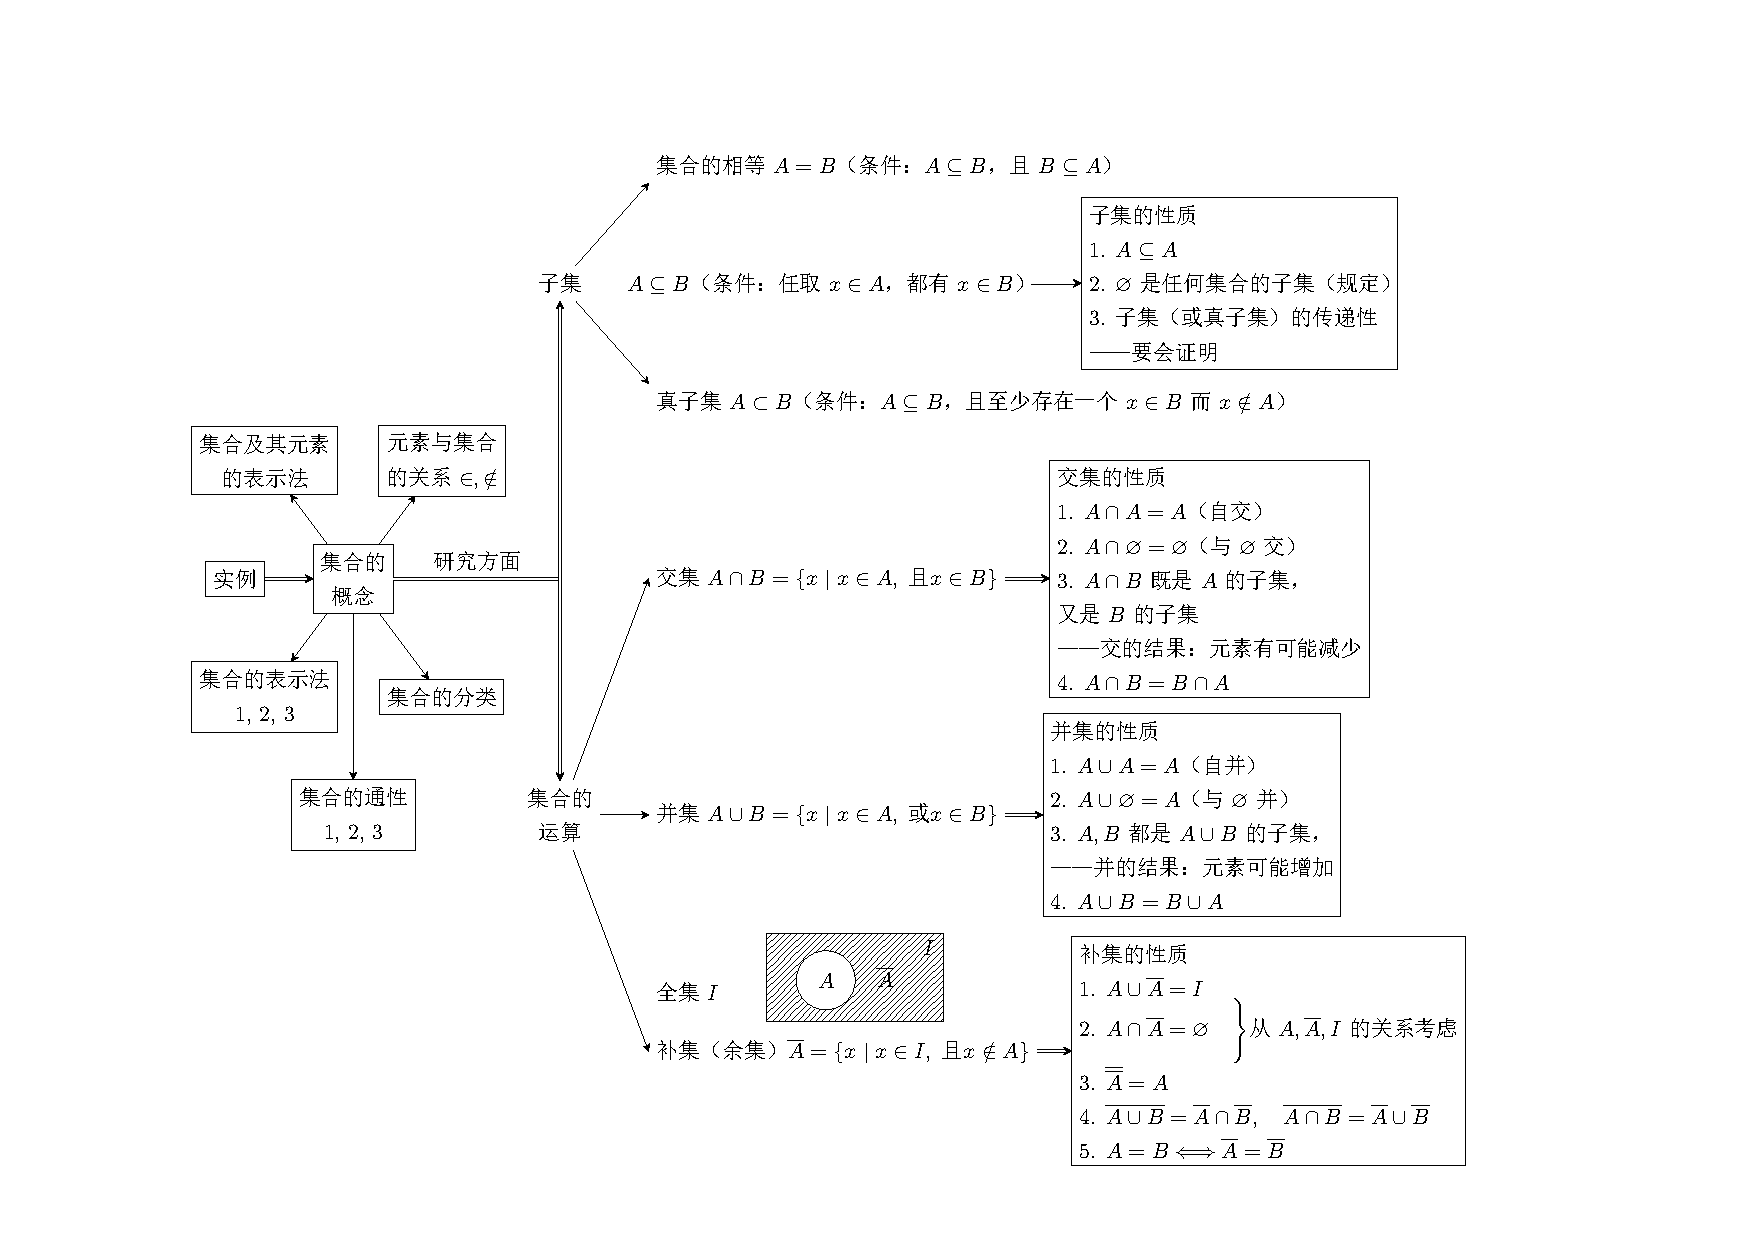
\includegraphics[scale=.7]{fig/fig1-8.pdf}
    \caption{}
\end{figure}
\end{landscape}


\subsection{几点说明}

\begin{enumerate}
    \item 要认真读书。既要对每个概念、符号、结论正确理
    解,正确表达,又要把它们之间逻辑上的联系弄清记牢。这
    就是常言所说的“既看树木,又见森林”。要弄清逻辑上的联
    系,一个有效的办法是根据讲课的顺序画出理论发展的逻辑
    结构图(如图1.8).

    经过这样整理后的知识,由于揭示了知识间的内在联系,理论发展的来龙去脉一目了然,每个知识点在系统中的
地位、作用比较清楚,因而能深化对理论的理解,有利于从
整体上掌握知识。结合这张图:
\begin{enumerate}[(1)]
\item 应能对每个概念正确叙述,并能指出它们在知识
系统中的地位与作用;
\item 应能通过对子、交、并、补集的图示法正确地掌
握它们的性质。
\end{enumerate}

\item 本章中要注意理解、掌握的数学思想有:
\begin{enumerate}[(1)]
 \item 用集合的观点处理问题的思想;
\item 把对象分类讨论的思想;
\item 数与形互相转化的思想。  
\end{enumerate}
\end{enumerate}



\section*{复习题一}
\begin{center}
    \bfseries A
\end{center}

\begin{enumerate}
    \item 已知$A=\{x\mid x\text{是小于6的自然数}\}$, 
    $B=\{x\mid x\text{是小于10的素数(质数)}\}$,  $C=\{x\mid x\text{是24和36的正的公约数}\}$。
    用列举法写出: 
\begin{enumerate}[(1)]
    \item $\{y\mid y\in A,\;\text{且} y\in C\}$;
    \item $\{y\mid y\in A,\;\text{或} y\in B\}$;
    \item $\{y\mid y\in B,\; \text{且}y\notin C\}$.
\end{enumerate}
  \item 已知$A=\{x\mid x=5k+1,\; k\in \Z\}$, $B=\{x\mid x=5k+2,\; k\in \Z\}$, $C=\{x\mid x=5k+3,\; k\in \Z\}$, $D=\{x\mid x=5k-1,\; k\in \Z\}$
  \begin{enumerate}[(1)]
    \item 将集合$A\cup B\cup C\cup D$化简。
    \item 填空:$A\cap B=\blank$, $C\cap D=\blank$。
  \end{enumerate}

\item  用适当的符号($\subset$, $=$, $\supset$)填空:
\begin{enumerate}[(1)]
    \item 已知$A=\{x\mid x=2k+1,\; k\in \Z\}$, $B=\{y\mid y=4k\pm 1,\; k\in \Z\}$, 则$A\blank B$;
    \item 已知$A=\{x\mid x\in\Z,\; x\ne 3n,\; n\in \Z\}$, $B=\{y\mid y=3n\pm 1,\; n\in \Z\}$, 则$A\blank B$;
    \item 已知$A=\{x\mid x=4n,\; n\in \Z\}$, $B=\{x\mid x=6n,\; n\in \Z\}$, 则$A\cap B=\blank $.
\end{enumerate}

\item 已知$A=\{x\mid x=4k,\; k\in \Z\}$, $B=\{x\mid x=4k+2,\; k\in \Z\}$,则$A\cup B=\blank$,$A\cap B=\blank$.

\item 已知$A=\left\{x\left|\; \left|x-\frac{1}{3}\right|>\frac{2}{3}\right.\right\}$, $B=\left\{x\mid |x-2|<3\right\}$,则$A\cap B=\blank$,$\overline{A}\cap \overline{B}=\blank$.

\item 用阴影表示:
\begin{enumerate}[(1)]
    \item $\overline{\overline{A}\cup B}$(其中$A\cap B\ne \emptyset$)
    \item $\overline{C\cap \overline{D}}$(其中$C\cap D\ne \emptyset$)
\end{enumerate}

\item 若$A=\{x\mid 2x^{2}+px+q=0\}$, $B=\{x\mid 6x^{2}+\left(2-p\right)x+5+q=0\}$,且$A \cap B=\left\{\frac{1}{2}\right\}$
,则$A\cup B=\blank$.
\item 设$A=\{-4, 2a-1,a^{2}\}$, $B=\{a-5,1-a,9\}$, 又已知
    $A\cap B=\{9\}$, 求$a$.
\end{enumerate}

\begin{center}
\bfseries B
\end{center}

\begin{enumerate}\setcounter{enumi}{8}
    \item 若$(x-1)^2+\sqrt{y+2}=0$
    的解集为$B$, $A=\{1,-2,3\}$,    则下列关系中正确的是(\qquad )
\begin{multicols}{4}
   \begin{enumerate}[(1)]
    \item $B\subset A$
    \item $B\in A$
    \item $B\cap A=\{1,-2\}$
    \item $B\cap A=\emptyset$
   \end{enumerate} 
\end{multicols}

\item 设$I=\{1,2,5,a^2-3a\}$, $A=\{2,5\}$, $B=\{a,5\}$, $\overline{A\cup B}=\{a-3\}$,$a$有可能取什么值。

\item 已知$I=\R$,$A=\{x\mid |x-a|<4\}$,$B=\{x\mid |x-2|>3\}$,且$A\cup B=\R$,求$a$的范围。
\item 已知$I=\R$,$A=\{x\mid |x-1|\ge a\}$,$B=\left\{x\left|\begin{cases}
    2x-1<3x+5\\ 5x-2<3x+6
\end{cases}\right.\right\}$,且$A\cap B=\emptyset$,求$a$的范围。

\end{enumerate}


\begin{center}
    \bfseries C
\end{center}

\begin{enumerate}\setcounter{enumi}{12}
    \item 设$S$为满足如下条件的自然数构成的集合:
    若$x\in S$, 则$(10-x)\in S$,
\begin{enumerate}[(1)]
\item 试求单元素集$S$;
\item 试求双元素集$S$;
\item 满足条件的集合$S$共有多少个?
\end{enumerate}

\end{enumerate}



 \chapter{映射与函数}

“函数”是近代数学中最重要的概念之一,在数学和其他
科学领域中有广泛的应用。

在初中,我们初步接触过函数,学习过正比例函数、反
比例函数、一次函数和二次函数。

本章首先学习映射的有关概念,然后以映射的观点研究
函数,使大家对函数的理解提到一个新水平。

\section{对应与映射}
在初中我们学过对应的个别例子。如,对于任何一个实
数$a$, 在数轴上都有唯一的一个点$A$和它对应;对于坐标平面
上任何一个点$P$, 都有唯一的有序实数对$(x,y)$和它对应。

“对应”也是数学中的原始概念。观察图2.1表示出的一
些对应可以看出,任何一个对应必须涉及两个集合$A$、$B$和
它们之间的对应法则(对应方法)$f$, 这三点称为\textbf{对应的三
要素}。

如果我们舍弃对应法则的具体内容,而仅仅从对应所涉
及的元素的个数上考虑这个对应是“几对几”的,那么不难看
出:对应(5)是“1对多”的;对应(2)、(4)是“多对1”的;对
应(1)、(3)是“1对1”的。其中,“1对1”和“多对1”这两类特
殊的对应——今后统称为映射——是我们研究的重点。抽出
这两类对应的共性,我们给出下面的:

\begin{thm}{定义1 }
    对于两个非空集合$A$、$B$, 如果任取集合$A$中的
一个元素,在对应法则$f$的作用下,在集合$B$中都有唯一元
素和它对应,这样的对应叫做\textbf{从集合$A$到集合$B$的映射},记
作$f:\; A\mapsto  B$.
\end{thm}

如果给定一个从集合$A$到集合$B$的映射,那么,与集合$A$
中的元素$x$对应的集合$B$中的元素$y$叫做$x$的\textbf{象},$x$叫做$y$的\textbf{原
象}。如图2.1中(1)这个映射,$A$中的元素1在$f$的作用下对
应$B$中的元素3(表示成
$f:\; 1\mapsto  3$),这里3是1的象,1是3的原象.

\begin{figure}[htp]
    \centering
\begin{tikzpicture}[>=stealth]
\begin{scope}
\draw(0,0)  ellipse (.8 and 2);
\draw(2,0)  ellipse (.8 and 2);
\node(A1) at (0,1){1};
\node(A2) at (0,0){2};
\node(A3) at (0,-1){3};
\node(B1) at (2,1){3};
\node(B2) at (2,0){5};
\node(B3) at (2,-1){7};
\draw[->](A1)--(B1);
\draw[->](A2)--(B2);
\draw[->](A3)--(B3);

\node at (1,2.5){$f:\; \text{乘}2+1$};
\node at (0,-2.35){$A$};
\node at (2,-2.35){$B$};
\node at (1,-2.75){$(1)$};
\end{scope}
\begin{scope}[xshift=4cm]
\draw(0,0)  ellipse (.8 and 2);
\draw(2,0)  ellipse (.8 and 2);
\node(A1) at (0,1.5){$+1$};
\node(A2) at (0,0.5){$-1$};
\node(A3) at (0,-.5){$+2$};
\node(A4) at (0,-1.5){$-2$};
\node(B1) at (2,1){1};
\node(B2) at (2,-1){4};
\draw[->](A1)--(B1);
\draw[->](A2)--(B1);
\draw[->](A3)--(B2);
\draw[->](A4)--(B2);

\node at (1,2.5){$f:\; \text{平方}$};
\node at (0,-2.35){$A$};
\node at (2,-2.35){$B$};
\node at (1,-2.75){$(2)$};
\end{scope}
\begin{scope}[xshift=8cm]
\draw(0,0)  ellipse (.8 and 2);
\draw(2,0)  ellipse (.8 and 2);
\node(A1) at (0,1.5){中};
\node(A2) at (0,0.5){俄};
\node(A3) at (0,-.5){美};
\node(A4) at (0,-1.5){日};
\node(B1) at (2,1.2){北京};
\node(B2) at (2,.6){莫斯科};
\node(B3) at (2,0){华盛顿};
\node(B4) at (2,-.6){东京};
\node(B5) at (2,-1.2){巴黎};
\draw[->](A1)--(B1);
\draw[->](A2)--(B2);
\draw[->](A3)--(B3);
\draw[->](A4)--(B4);
\node at (1,2.5){$f:\; \text{找首都} $};
\node at (0,-2.35){$A$};
\node at (2,-2.35){$B$};
\node at (1,-2.75){$(3)$};
\end{scope}

\begin{scope}[yshift=-6.5cm]
\draw(0,0)  ellipse (.8 and 2);
\draw(2,0)  ellipse (.8 and 2);
\node(A1) at (0,1.75){1};
\node(A2) at (0,1.25){2};
\node(A3) at (0,.75){3};
\node(A4) at (0,.25){4};
\node(A5) at (0,-.25){5};
\node(A6) at (0,-.75){6};
\node(A7) at (0,-1.25){7};
\node(A8) at (0,-1.75){8};

\node(B1) at (2,1){0};
\node(B2) at (2,0){1};
\node(B3) at (2,-1){2};
\draw[->](A1)--(B2);
\draw[->](A2)--(B1);
\draw[->](A3)--(B2);
\draw[->](A4)--(B1);
\draw[->](A5)--(B2);
\draw[->](A6)--(B1);
\draw[->](A7)--(B2);
\draw[->](A8)--(B1);

\node at (1,2.5){$f:\; \text{除以2的余数}$};
\node at (0,-2.35){$A$};
\node at (2,-2.35){$B$};
\node at (1,-2.75){$(4)$};
\end{scope}
\begin{scope}[xshift=4cm, yshift=-6.5cm]
\draw(0,0)  ellipse (.8 and 2);
\draw(2,0)  ellipse (.8 and 2);
\node(A1) at (0,1){$1$};
\node(A2) at (0,0){$4$};
\node(A3) at (0,-1){$9$};
\node(B1) at (2,1.25){$-1$};
\node(B2) at (2,.75){$+1$};
\node(B3) at (2,.25){$-2$};
\node(B4) at (2,-.25){$+2$};
\node(B5) at (2,-.75){$-3$};
\node(B6) at (2,-1.25){$+3$};

\draw[->](A1)--(B1);
\draw[->](A1)--(B2);
\draw[->](A2)--(B3);
\draw[->](A2)--(B4);
\draw[->](A3)--(B5);
\draw[->](A3)--(B6);


\node at (1,2.5){$f:\; \text{开平方}$};
\node at (0,-2.35){$A$};
\node at (2,-2.35){$B$};
\node at (1,-2.75){$(5)$};
\end{scope}
\begin{scope}[xshift=8cm, yshift=-6.5cm]
\draw(0,0)  ellipse (.8 and 2);
\draw(2,0)  ellipse (.8 and 2);
\node(A1) at (0,1.5){$a$};
\node(A2) at (0,0.5){$b$};
\node(A3) at (0,-.5){$c$};
\node(A4) at (0,-1.5){$d$};
\node(B1) at (2,1.5){$x$};
\node(B2) at (2,.5){$y$};
\node(B3) at (2,-.5){$z$};
\node(B4) at (2,-1.5){$\omega$};
\draw[->](A1)--(B1);
\draw[->](A1)--(B2);
\draw[->](A2)--(B3);
\draw[->](A3)--(B3);
\node at (1,2.5){$f$};
\node at (0,-2.35){$A$};
\node at (2,-2.35){$B$};
\node at (1,-2.75){$(6)$};
\end{scope}
\end{tikzpicture}
    \caption{}
\end{figure}



\begin{note}
\begin{enumerate}
    \item “任取$A$中的一个元素$x$, 都存在
$y\in B$,……”,这一
点讲的是在$A$中取元的\textbf{任意性}。很明显,图2.1中的六个对
应中,除(6)以外都具有取元的任意性。
\item 当$A$中的元素$x$取定后,与其对应的$B$中的元素$y$是
唯一的(即不存在两个或两个以上的$y$对应于同一个$x$), 这
一点讲的是成象的\textbf{唯一性}。很明显,图2.1中的六个对应中
只有(1)、(2)、(3)、(4)才具有成象的唯一性。

从定义可以看出,\textbf{取元的任意性和成象的唯一性刻画了
映射这个概念的本质属性}。因此,欲判断某个对应是不是映
射,只要检查一下这“\textbf{两条通性}”是否同时具备就可以了。

此外,对映射来说还需理解:

\item 有的映射是$B$中的每个元素都有原象(这一种称为\textbf{到
$B$上的映射}),有的是$B$中的元素至少有一个没有原象(这一
种称为\textbf{到$B$内的映射})。很明显(1)、(2)是到$B$上的映射,
(3)、(4)是到$B$内的映射。
\item 对映射来说,$A$、$B$不一定是数的集合,如(3).
\item 对映射来说,符号$f:\; x\mapsto  y$意味着对应法则$f$把元素$x$
映射为$y$(也就是在$f$的作用下,$x$的象是$y$,$y$
的原象是$x$). 符号$f:\; A\mapsto  B$
意味着对应法则$f$把集合$A$映射为$B'$, 而$B'\subseteq B$(也就是在$f$的作用下,$A$中元素的象的集合是$B'$, 而$B'$
是$B$的子集)。
\end{enumerate}
\end{note}    



\begin{example}
    下列从$A$到$B$的对应中,哪些是映射,哪些不是映
射?(要简述理由)
\begin{enumerate}[(1)]
    \item $A=\Z,\; B=\Z,\; f:\, x\mapsto  y=3x$;
    \item $A=\Q,\; B=\Q,\; f:\, x\mapsto  y=x^3$;
    \item $A=\R,\; B=\R,\; f:\, x\mapsto  y=\sqrt{x}$;
    \item $A=\{0,2,4\},\; B=\{0,\pm\sqrt{2},\pm 2\},\; f:\, \text{找平方根}$;
\end{enumerate}
\end{example}

\begin{analyze}
    据定义1, 一个对应若同时具有取元的任意性和
成象的唯一性,它就是映射,否则就不是映射。
\end{analyze}

\begin{solution}
\begin{enumerate}[(1)]
    \item 当任给$x\in A$时,存在唯一的
$3x\in\Z$,即$y\in B$,

$\therefore\quad $对应(1)是映射。

\item 当任给$x\in A$时,存在唯一的
$x^3\in\Q$,即$y\in B$,

$\therefore\quad $对应(2)是映射。
\item 当$x\in\R^-\subset \R$时,$x$的算术平方根无意义,也就是
在对应法则$f$的作用下,$x$在$B$中没有象,所以,不具备取元
的任意性,从而对应(3)不是映射。
\item 当$x$为2或4时,在$f$作用下,$x$在$B$中有两个象
$\pm\sqrt{x}$. 所以,不具备成象的唯一性,从而(4)也不是映
射。
\end{enumerate}
\end{solution}

\section*{习题一}
\begin{center}
    \bfseries A
\end{center}

\begin{enumerate}
    \item 下列从$A$到$B$的对应中,哪些是映射?哪些不是?简述理由.
\begin{enumerate}[(1)]
    \item $A=\R$, $B=\R^+$, $f:\;\text{取绝对值}$;
    \item $A=\R$, $B=\R$, $f:\;\text{取倒数}$;
    \item $A=\N$, $B=\R$, $f:\;\text{2倍加1}$;
    \item $A=\{30^{\circ},45^{\circ},90^{\circ},150^{\circ}\}$, $B=\left\{\frac{1}{2},\frac{\sqrt{2}}{2},1\right\}$, $f:\;\text{求正弦}$.
\end{enumerate}

\item 对于映射$f:\; A\mapsto  B$, 判断下列命题的真假,并简述理由:
\begin{enumerate}[(1)]
\item $A$中的每一个元素在$B$中有且仅有一个象;
\item $B$中的元素在$A$中都有原象;
\item $B$中的元素在$A$中可以有两个以上的原象,也可以
无原象.
\end{enumerate}

\item 设$A=\{x\mid x\ge 0\}$, $B=\{x\mid x\in\R\}$
,下列对应法则中,由
(\quad )确定的对应是从$A$到$B$的映射。
\begin{enumerate}[(1)]
    \item $f:\; x\mapsto  x$的平方根。
\item $f:\; x\mapsto  y=\frac{1}{x}$
\item $f:\; x\mapsto  x\text{的算术平方根}$
\item $f:\; x\mapsto  y=\sqrt{x-3}$.
\end{enumerate}
\end{enumerate}

\begin{center}
    \bfseries B
\end{center}

\begin{enumerate}\setcounter{enumi}{3}
    \item 设$A=\{a,b\}$, $B=\{c,d\}$,试用图示法表明最多可以构造多少种从$A$到$B$的映射?
\end{enumerate}

\section{一一映射和逆映射}
观察下面三个映射(图2.2):
\begin{enumerate}[(1)]
\item (甲)、(乙)相比,(甲)具有什么特点?
\item (甲)、(丙)相比,(甲)具有什么特点?
\end{enumerate}

(甲)、(乙)相比,(甲)的特点是“1对1”的,即$A$中不同元
素,在$B$中有不同的象;

(甲)、(丙)相比,(甲)的特点是“到上”的,即$B$中的
每个元素在$A$中都有原象。

象(甲)这样的具有上述两个特点的映射称为从$A$到$B$上
的一一映射。


\begin{figure}[htp]
    \centering
\begin{tikzpicture}[>=stealth]
\begin{scope}
\draw(0,0)  ellipse (.8 and 2);
\draw(2,0)  ellipse (.8 and 2);
\node(A1) at (0,1){$a$};
\node(A2) at (0,0){$b$};
\node(A3) at (0,-1){$c$};
\node(B1) at (2,1){$x$};
\node(B2) at (2,0){$y$};
\node(B3) at (2,-1){$z$};
\draw[->](A1)--(B1);
\draw[->](A2)--(B2);
\draw[->](A3)--(B3);
\node at (0,2.35){$A$};
\node at (2,2.35){$B$};
\node at (1,-2.35){(甲)};
\end{scope}
\begin{scope}[xshift=4cm]
\draw(0,0)  ellipse (.8 and 2);
\draw(2,0)  ellipse (.8 and 2);
\node(A1) at (0,1.2){$p$};
\node(A2) at (0,0.6){$q$};
\node(A3) at (0,0){$r$};
\node(A4) at (0,-.6){$s$};
\node(A5) at (0,-1.2){$t$};
\node(B1) at (2,.8){$m$};
\node(B2) at (2,-.8){$n$};
\draw[->](A1)--(B1);
\draw[->](A2)--(B1);
\draw[->](A3)--(B2);
\draw[->](A4)--(B2);
\draw[->](A5)--(B2);

\node at (0,2.35){$C$};
\node at (2,2.35){$D$};
\node at (1,-2.35){(乙)};
\end{scope}
\begin{scope}[xshift=8cm]
\draw(0,0)  ellipse (.8 and 2);
\draw(2,0)  ellipse (.8 and 2);
\node(A1) at (0,1){1};
\node(A2) at (0,0){2};
\node(A3) at (0,-1){3};
\node(B1) at (2,1.2){10};
\node(B2) at (2,.6){20};
\node(B3) at (2,0){30};
\node(B4) at (2,-.6){40};
\node(B5) at (2,-1.2){50};
\draw[->](A1)--(B1);
\draw[->](A2)--(B2);
\draw[->](A3)--(B3);

\node at (0,2.35){$E$};
\node at (2,2.35){$F$};
\node at (1,-2.35){(丙)};
\end{scope}
\end{tikzpicture}
    \caption{}
\end{figure}

\begin{thm}{定义2}
     若映射$f:\; A\mapsto  B$
还同时具有下面两种属性:
\begin{enumerate}[(1)]
\item $A$中不同的元素,在$B$中有不同的象(这一点称为
\textbf{单射});
\item $B$中每个元素,在$A$中都有原象(这一点称为\textbf{满
射}).
\end{enumerate}
则称$f$是\textbf{从$A$到$B$上的一一映射}。
\end{thm}

\begin{note}
\begin{enumerate}
    \item 一一映射是同时满足性质(1)、(2)的映射,所以,
    它是一种特殊的映射。因此,欲判断一个对应是一一映射,应
    首先断定它是映射,进而还必须再断定它还是单射和满射。
    \item 性质(1)(单射)实质上是说映射是“1对1”的,它否定
    了“多对1”的可能性;性质(2)(满射)是说映射是“到上”的,
    它否定了“到内”的可能性。
\end{enumerate}
\end{note}

\begin{thm}{思考题}
    设$A=\N$, $B=\{3, 5,7,9,\ldots,(2n+1),\ldots\}$, $f:
   \; x\mapsto  y=2x+1$.
\begin{enumerate}[(1)]
    \item 由$f$确定的对应是从$A$到$B$的映射吗?
    \item 由$f$确定的对应是从$A$到$B$上的一一映射吗?
\end{enumerate}
\end{thm}


\begin{solution}
 \begin{enumerate}[(1)]
    \item 任取$x\in A$, 都有唯一的
$y=2x+1\in B$,所以
由$f$确定的对应是从$A$到$B$的映射。
\item 取$y_0=1\in B$,按照对应法则
$f:\; y=2x+1$,在$A$中找不到$y_0$
的原象,即由$f$确定的映射不是满射,所以,
这个映射不是从$A$到$B$上的一一映射。
 \end{enumerate}   
\end{solution}

\begin{example}
    $A=\R$, $B=\{y\mid y\ge 0\}$, $f:\;x\mapsto  y=x^2$.
\begin{enumerate}[(1)]
\item 由$f$确定的这个对应是从$A$到$B$的映射吗?
\item 由$f$确定的这个对应是从$A$到$B$上的一一映射吗?
\end{enumerate}
\end{example}

\begin{solution}
\begin{enumerate}[(1)]
    \item 不难看出,这个对应既满足取元的任意性,
    又满足成象的唯一性,所以是从$A$到$B$的映射。
    \item 由于在$A$中两个不同的元素$x,-x\; (x\ne 0)$
    在$B$中有相同的象$x^2$
    ,即对应不是单射,所以这个对应不是从
    $A$到$B$上的一一映射。
\end{enumerate}

\end{solution}

由上可以看出理论发展的线索是:
\begin{center}
    \begin{tikzpicture}[>=stealth]
\node(A) at (0,0)[draw]{\huge 对应};
\node(B) at (5,0)[draw]{\huge 映射};
\node(C) at (9.5,0)[draw]{\huge 一一映射};
\draw[->](A)--node[above]{取元的任意性}node[below]{成象的唯一性}(B);
\draw[->](B)--node[above]{单射}node[below]{满射}(C);

    \end{tikzpicture}
\end{center}

\begin{thm}{思考题}
    观察下列三个映射(图2.3), 若将其中的元素间的对应
指向(即箭头指向)按原路全部逆反后,哪个映射逆反后
得到的仍然是映射?
\end{thm}

很明显,情况(甲)逆反后得到的对应仍然是映射;情
况(乙)由于是非单射,$B$中至少有一个元素(如$m$)有两个
或多个原象,指向逆反后必破坏成象的唯一性,得到的对
应就不是映射;情况(丙)由于是非满射,$B$中至少有一个元
素无原象,指向逆反后必破坏取元的任意性,所以得到的也
不是映射。



\begin{figure}[htp]
    \centering
\begin{tikzpicture}[>=stealth]
\begin{scope}
\draw(0,0)  ellipse (.8 and 2);
\draw(2,0)  ellipse (.8 and 2);
\node(A1) at (0,1.2){$x_1$};
\node(A2) at (0,0.4){$x_2$};
\node(A3) at (0,-.4){$x_3$};
\node(A4) at (0,-1.2){$x_4$};
\node(B1) at (2,1.2){$y_1$};
\node(B2) at (2,.4){$y_2$};
\node(B3) at (2,-.4){$y_3$};
\node(B4) at (2,-1.2){$y_4$};
\draw[->](A1)--(B1);
\draw[->](A2)--(B3);
\draw[->](A4)--(B4);
\draw[->](A3)--(B2);
\node at (1,2.35){$f$};
\node at (0,-2.35){$A$};
\node at (2,-2.35){$B$};
\node at (1,-3){(甲)一一映射};
\end{scope}
\begin{scope}[xshift=4cm]
\draw(0,0)  ellipse (.8 and 2);
\draw(2,0)  ellipse (.8 and 2);
\node(A1) at (0,1){$p$};
\node(A2) at (0,0){$q$};
\node(A3) at (0,-1){$r$};
\node(B1) at (2,.7){$m$};
\node(B2) at (2,-.7){$n$};
\draw[->](A1)--(B1);
\draw[->](A2)--(B1);
\draw[->](A3)--(B2);
\node at (1,2.35){$f$};
\node at (0,-2.35){$A$};
\node at (2,-2.35){$B$};
\node at (1,-3){(乙)非单射};
\end{scope}
\begin{scope}[xshift=8cm]
\draw(0,0)  ellipse (.8 and 2);
\draw(2,0)  ellipse (.8 and 2);
\node(A1) at (0,1){$a$};
\node(A2) at (0,0){$b$};
\node(A3) at (0,-1){$c$};
\node(B1) at (2,1.2){$x$};
\node(B2) at (2,.4){$y$};
\node(B3) at (2,-.4){$z$};
\node(B4) at (2,-1.2){$\omega$};
\draw[->](A1)--(B1);
\draw[->](A2)--(B2);
\draw[->](A3)--(B3);

\node at (1,2.35){$f$};
\node at (0,-2.35){$A$};
\node at (2,-2.35){$B$};
\node at (1,-3){(丙)非满射};
\end{scope}
\end{tikzpicture}
    \caption{}
\end{figure}


\begin{thm}{定义3}
     对于一一映射$f:\; A\mapsto  B$,其中$f:\; x\mapsto  y$ 
($x\in A$),
若使$A$中的元素$x$与它在$B$中的象$y$对应(即使
$y\mapsto  x$ ($y\in B$)),这样得到的映射称为映射$f:\; A\mapsto  B$的
\textbf{逆映射},记作
$f^{-1}:\; B\mapsto  A$, 其中
$f^{-1}:\; y\mapsto  x$($y\in B$).
\end{thm}

\begin{note}
\begin{enumerate}
    \item 只有一一映射才存在逆映射;
    \item  一一映射的逆映射仍然是一一映射;
    \item  一个映射与它的逆映射互为逆映射.
\end{enumerate}
\end{note}

\begin{example}
    下列映射是否存在逆映射?简述理由。若存在,试
求之:
\begin{enumerate}[(1)]
    \item $A=\R$, $B=\R$, $f:\; A\mapsto  B$, $f:\; x\mapsto  y=2x-3\; (x\in A)$;
    \item $A=\{x\mid x>0\}$, $B=\{y\mid y>0\}$, $f:\; A\mapsto  B$, $f:\; x\mapsto  y=\frac{1}{x}\; (x\in A )$;
    \item $A=\R$, $B=\{y\mid y\ge 0\}$, $f:\; A\mapsto  B$, $f:\; x\mapsto  y=x^2\; (x\in A)$.
\end{enumerate}
\end{example}

\begin{solution}
\begin{enumerate}[(1)]
    \item $\because\quad$ 映射$\map{f}{A}{B}$是从$A$到$B$上的一一映射,
    
    $\therefore\quad $它存在逆映射$\map{f^{-1}}{B}{A}$
    ,其中$\map{f^{-1}}{y}{x=\frac{y+3}{2}}\; (y\in B)$

    \item $\because\quad$ 映射$\map{f}{A}{B}$是从$A$到$B$上的一一映射,
   
    $\therefore\quad $ 它存在逆映射$\map{f^{-1}}{B}{A}$
    ,其中$\map{f^{-1}}{y}{x=\frac{1}{y}}\; (y\in B)$

    \item $\because\quad$ 映射$\map{f}{A}{B}$不是从$A$到$B$上的一一映射,事
    实上,$A$中的元素$\pm x\; (x\ne 0)$
    在$B$中有同一个象$x^2$, 从而$\map{f}{A}{B}$
    不是单射,

$\therefore\quad \map{f}{A}{B}$不存在逆映射。
\end{enumerate}
\end{solution}

\section*{习题二}
\begin{center}
    \bfseries A
\end{center}

\begin{enumerate}
    \item “对于映射$\map{f}{A}{B}$
    ,若$B$中每一个元素在$A$中有且只有一
    个原象,则$\map{f}{A}{B}$
    一定是从$A$到$B$上的一一映射”这句话
    对吗?
    \item 下列各表分别表示集合$A$(元素为$a$)到集合$B$(元素为$b$)的
    一个映射,判断这些映射是不是从$A$到$B$上的一一映射?
\begin{multicols}{2}
(1) \begin{tabular}{|c|c|c|c|c|}
\hline
    $a$&1&2&3&4\\
    \hline
$b$&$-1$&$-1$&$-1$&$-1$\\
\hline
\end{tabular}

(2) \begin{tabular}{|c|c|c|c|c|}
    \hline
        $a$&3&4&5&6\\
        \hline
    $b$&$2$&$3$&$2$&$4$\\
    \hline
    \end{tabular}

(3) \begin{tabular}{|c|c|c|c|c|}
    \hline
        $a$&1&2&3&4\\
        \hline
    $b$&$3$&$6$&$9$&$12$\\
    \hline
    \end{tabular}

(4) \begin{tabular}{|c|c|c|c|c|c|}
    \hline
        $a$&3&4&5&6\\
        \hline
    $b$&$2$&$3$&$4$&$5$&6\\
    \hline
    \end{tabular}
\end{multicols}

\item 若$A=\{\text{整数}\}$,$B=\{\text{非负整数}\}$, $\map{f}{x}{y=|x|}\; (x\in A)$
\begin{enumerate}[(1)]
    \item 这个对应是不是从$A$到$B$的映射?
    \item 这个对应是不是从$A$到$B$上的一一映射?
\end{enumerate}
\end{enumerate}

\begin{center}
    \bfseries B
\end{center}

\begin{enumerate}\setcounter{enumi}{3}
    \item 下列映射$\map{f}{A}{B}$
    有逆映射吗?若有试求之。
\begin{enumerate}[(1)]
    \item $A=\{x\mid x\ge 1\}$, $B=\{y\mid y\ge 0\}$, $\map{f}{x}{y=\sqrt{x-1}}$;
    \item $A=\{x\mid x\in\R,\; x\ne 0\}$, $B=\{y\mid y\in\R,\; y\ne 1\}$, $\map{f}{x}{y=1-\frac{1}{x}}$;
    \item $A=\{1,2,3,4,5\}$, $B=\{2,9,28,65,126\}$, $\map{f}{x}{y=x^3+1}$;
    \item $A=\{x\mid x\le 0\}$, $B=\{y\mid y\ge 3\}$, $\map{f}{x}{y=x^2+3}$.
\end{enumerate}

\item 下列各映射,是否存在逆映射?若有,试求之;若不存
在,说明理由。
\begin{enumerate}[(1)]
    \item $A=\Q$, $B=\R$,映射$\map{f}{A}{B}$,$\map{f}{x}{y=2x}$;
    \item $A=\{x\mid x\in\Z\}$, $B=\{y\mid y\in\Z,\; y\ge 0\}$,映射
    $\map{f}{A}{B}$,$\map{f}{x}{y=|x|}$;
\item $A=\R$, $B=\R$,映射$\map{f}{A}{B}$,$\map{f}{x}{y=x^3}$.
\end{enumerate}

\item $A=\{a,b\}$, $B=\{c,d\}$,最多可以构造多少种从$A$到$B$
的一一映射?试用图示法表示之。
\item 已知映射$\map{f}{A}{B}$. 其中$\map{f}{x}{y=2x+1}$, $B=\{3,5,
7\}$,
满足条件的集合$A$共有多少个?试写出它们。

\end{enumerate}

\section{函数}

\subsection{函数的定义}
函数是数学中极为重要的概念。在初中,我们曾初步接
触过它。

在一个变化过程中,如果有两个变量$x$、$y$, 对于变量$x$
在允许值范围内的每一个值,按照某种对应法则,变量$y$都
有唯一确定的值和它对应,就说$y$是$x$的\textbf{函数}。

以映射的观点来看,函数关系实质上是从一个数集到另
一个数集的映射。

\begin{thm}{定义4}
   若$A$、$B$都是非空数集,称映射$\map{f}{A}{B}$
(其中$\map{f}{x}{y}$)
为\textbf{定义在$A$上的函数},记作
\[y=f(x),\qquad x\in A\]
读作“$y$是$x$的函数,$x\in A$”\footnote{$f$是英语单词function(函数)的词头字母。$f(x)$实际上是“function
of $x$”的缩写.}。$A$称为函数的定义域(常用大
写英文字母$D$来表示\footnote{$D$是英语单词Definition(定义)的词头字母。}),$x$的象的集合$B'\; (B'\subseteq B)$
称为函数的\textbf{值域}。当取$x=a$
时,$x$的象$f(a)$称为$f(x)$
在$x=a$处的\textbf{函数值},显然有
$f(a)\in B'$
。很明显,这里函数的定义域$D$
就是初中讲过的自变量$x$的取值范围,函数的值域$B'$就是因
变量$y$的取值范围。
\end{thm}

例如,下面两个对应(图2.4)
\begin{figure}[htp]
    \centering
\begin{tikzpicture}[thick,>=stealth, scale=.9]
\begin{scope}
\draw(0,0)  ellipse (.8 and 2);
\draw(2,0)  ellipse (.8 and 2);
\node(A1) at (0,1){$-1$};
\node(A2) at (0,-1){$1$};
\node(B1) at (2,1){$1$};
\node(B2) at (2,-1){$0$};
\draw[->](A1)--(B1);
\draw[->](A2)--(B1);
\node at (1,2.35){$f:\; \text{平方}$};
\node at (1,-2.35){(甲)};
\end{scope}
\begin{scope}[xshift=5cm]
\draw(0,0)  ellipse (.8 and 2);
\draw(2,0)  ellipse (.8 and 2);
\node(A1) at (0,1){$-1$};
\node(A2) at (0,0){$0$};
\node(A3) at (0,-1){$1$};
\node(B1) at (2,1){$1$};
\node(B2) at (2,-1){$0$};
\draw[->](A1)--(B1);
\draw[->](A3)--(B1);
\draw[->](A2)--(B2);
\node at (1,2.35){$f:\; \text{平方}$};
\node at (1,-2.35){(乙)};
\end{scope}
\end{tikzpicture}
    \caption{}
\end{figure}

都是从数集到数集的映射,因而都是函数,而且,这两个
函数还具有相同的对应法则$f$. 所不同的是函数(甲)的
定义域是$\{-1,1\}$, 函数(乙)的定义域是$\{-1,0,
1\}$. 很明显,由于定义域不同,即使对应法则相同,也导
致了这两个函数的值域一个是$\{1\}$, 而另一个是$\{1,0\}$. 
由此可见,确定一个函数最根本的要素是$D$与$f$. 当$D$与$f$给
定以后,值域随之而定。

对定义4应着重理解:
\begin{enumerate}
    \item 函数是从数集到数集的映射(当然这是特殊的映
    射),因此要判断一个对应是不是给出了函数关系,根本还
    是要看对应是否具有取元的任意性和成象的唯一性。
    \item 给出一个函数最要紧的是必须给出定义域$D$与对应
    法则$f$. $D$与$f$都相同的两个函数一定是同一个函数。例如,
    $y=f(x),\; x\in D$与$V=f(t),\; t\in D$
    就表示同一个函数(虽然
    表示变量的字母不同,但这无关紧要)。
\end{enumerate}

\subsection{函数的定义域}
上面已经谈到,表示一个函数必须同时给出对应法则$f$
和定义域$D$. 但在用解析法表示函数时又常常只给出解析式,
此时意味着(约定)函数的定义域$D$是使解析式有意义的自
变量$x$的集合。
\begin{itemize}
    \item 若解析式是分式时,应该使分母$\ne 0$;
    \item 若解析式是偶次方根时,应使被开方数$\ge 0$;
    \item 若解析式是由实际问题建立的,还应考虑解析式的实际
意义。
\end{itemize}

\begin{example}
    求下列函数的定义域:
\begin{multicols}{2}
\begin{enumerate}[(1)]
    \item $f(x)=kx+b\quad (k\ne 0)$;
    \item $f(x)=\frac{k}{x}\quad (k\ne 0)$;
    \item $f(x)=\frac{1}{x+2}$;
    \item $f(x)=\sqrt{3x+2}$;
    \item $f(x)=\sqrt{x+1}+\frac{1}{1-x}$;
    \item $f(x)=\sqrt{2-3x}+\sqrt{x+5}$.
\end{enumerate}
\end{multicols}
\end{example}

\begin{analyze}
    这些函数只给出了对应法则,应按上述约定求它
的定义域$D$.
\end{analyze}

\begin{solution}    
\begin{enumerate}[(1)]
    \item $D=\R$.
    \item $D=\{x\mid x\in\R,\; x\ne 0\}=(-\infty,0)\cup(0,+\infty)$.
    \item 欲使$f(x)$有意义,需使$x+2\ne 0\Longrightarrow x\ne -2$,
    
$\therefore\quad D=\{x\mid x\in\R,\; x\ne -2\}=(-\infty,-2)\cup(-2,+\infty)$.

\item 欲使$f(x)$有意义,需使$3x+2\ge 0\Longrightarrow x\ge -\frac{2}{3}$,
    
$\therefore\quad D=\left\{x\, \Big|\, x\in\R,\; x\ge -\frac{2}{3}\right\}=\left[-\frac{2}{3},+\infty\right)$.

\item 欲使$f(x)$有意义,需使
\[\begin{cases}
    x+1\ge 0\\
    1-x\ne 0
\end{cases},\qquad \text{即}\; \begin{cases}
    x\ge -1\\x\ne 1
\end{cases}\]
$\therefore\quad D=\{x\mid x\in\R,\; x\ge -1,\; x\ne 1\}=[-1,1)\cup(1,+\infty)$.
\item 欲使$f(x)$有意义,需使
\[\begin{cases}
    2-3x\ge 0\\
    x+5\ge 0
\end{cases},\qquad \text{即}\; \begin{cases}
    x\le \frac{2}{3}\\x\ge -5
\end{cases}\]
$\therefore\quad D=\left(-5,\frac{2}{3}\right)$.
\end{enumerate}
\end{solution}    

\subsection{函数图象的画法}
我们知道,函数的图象,就是平面上的点集$\{(x,y) \text{点}\mid y=f(x),\; x\in D\}$, 因此画图象最基本的方法是\textbf{描点法}:列表,描点,将描出的点依次连接成光滑曲线。

\begin{example}
    画出下列函数的图象:
\begin{multicols}{2}
    \begin{enumerate}[(1)]
    \item $f_1(x)=\frac{1}{x},\quad x\in[-2,)\cup (0,8)$;
    \item $f_2(x)=\frac{1}{2}x-1,\quad x\in (-2,4]$.
\end{enumerate}
\end{multicols}
\end{example}


\begin{analyze}
应注意$f_1(x)$的图 象是反比 例函数图象上的一
    段,$f_2(x)$ 的图象是一次函数图象上的一段。
\end{analyze}

\begin{figure}[htp]
    \centering
\begin{minipage}{.45\textwidth}
\begin{tikzpicture}[scale=.60, >=stealth]
    \draw[->](-4,0)--(5,0)node[below]{$x$};
    \draw[->](0,-4)--(0,5)node[left]{$y$};
\draw[very thick, domain=-2:-.25, smooth]plot(\x, 1/\x);
\draw[very thick, domain=.25:3, smooth]plot(\x, 1/\x);
\node at (0,0)[below left]{$O$};
\foreach \x in {-3,-2,...,4}
{
    \draw(-.2,\x)--(0,\x);
    \draw(\x,.2)--(\x,0);
}
\node at (1,0)[below]{1};
\node at (-.2,1)[left]{1};
\node at (1,1)[above right]{$(1,1)$};
\node at (-1,-1)[below left]{$(-1,-1)$};
\draw[fill](1,1)circle (.1);
\draw[fill](-1,-1)circle (.1);
\draw[fill](-2,-.5)circle (.1);
\draw[fill](3,1/3)circle (.1);
\draw[fill](2,.5)circle (.1);
\draw[fill](1/2,2)circle (.1);
\draw[fill](-1/2,-2)circle (.1);


\end{tikzpicture}
    \caption{}
\end{minipage}
    \hfill
\begin{minipage}{.45\textwidth}
    \begin{tikzpicture}[scale=.60, >=stealth]
        \draw[->](-4,0)--(5,0)node[below]{$x$};
        \draw[->](0,-4)--(0,5)node[left]{$y$};
\node at (0,0)[below left]{$O$};
\draw[very thick, domain=-2:4, smooth]plot(\x, 0.5*\x-1);
\foreach \x in {-3,-2,...,4}
{
    \draw(-.2,\x)--(0,\x);
    \draw(\x,.2)--(\x,0);
}
\node at (1,0.2)[above]{1};
\node at (-.2,1)[left]{1};
\draw[fill](-2,-2)circle (.1);
\draw[fill](4,1)circle (.1);

\end{tikzpicture}
    \caption{}
\end{minipage}
    \label{}
\end{figure}

\begin{solution}
\begin{enumerate}[(1)]
    \item 列表
\begin{tabular}{c|ccccccc}
    \hline
$x$ & $-2$ &$-1$&$-\tfrac{1}{2}$&$\tfrac{1}{2}$&1&2&3\\
\hline
$y$ & $-\tfrac{1}{2}$&$-1$&$-2$&2&1&$\tfrac{1}{2}$&$\tfrac{1}{3}$\\
\hline
\end{tabular}

将对应的$(x,y)$坐标平面上描点、连线(图2.5)就得到了
$f_1(x)$的图象。
\item  同理可以作出$f_2(x)$的图象(图2.6).
\end{enumerate}
\end{solution}



   

\begin{note}
    作出的函数的图象:
\begin{enumerate}[(1)]
\item 必须能体现出函数的本质属性,因此应先分析函
数的性质再作图;
\item 图象上特殊点(包括端点)的位置和标记应准确
(闭区间的端点应画实心点,开区间的端点应画空心点);
\item 坐标轴与单位长应标出。
\end{enumerate}
\end{note}

一般来说,完成画图后对上述三点进行一次检查是必要
的。


\begin{example}
    画出下列函数的图象,并指出哪一个与$y=x$是同一个函数:
\begin{multicols}{2}
\begin{enumerate}[(1)]
    \item $y=\left(\sqrt{x}\right)^2$;
    \item $y=\frac{x^2}{x}$;
    \item $y=\sqrt[3]{x^3}$;
    \item $y=\sqrt{x^2}$.
\end{enumerate}
\end{multicols}
\end{example}

\begin{analyze}
    应先化简这些解析式再作图。
\end{analyze}

\begin{solution}
\begin{multicols}{2}
\begin{enumerate}
    \item $y=x\quad (x\ge 0)$;
    \item $y=x\quad (x\ne 0)$;
    \item $y=x\quad (x\in \R)$;
    \item $y=|x|=\begin{cases}
        x,&x\ge 0\\ -x, &x<0
    \end{cases}$.
\end{enumerate}
\end{multicols}
作图如下(图2.7):
\begin{figure}[htp]
    \centering
\begin{tikzpicture}[>=stealth]
\begin{scope}
\draw[->](-1,0)--(1.5,0)node[below]{$x$};
\draw[->](0,-1)--(0,1.5)node[left]{$y$};
\node at (0,0)[below right]{$O$};
\draw[thick](0,0)--(1.25,1.25);
\node at (0,-1.5){(1)};

\end{scope}
\begin{scope}[xshift=3cm]
    \draw[->](-1,0)--(1.5,0)node[below]{$x$};
    \draw[->](0,-1)--(0,1.5)node[left]{$y$};
    \node at (0,0)[below right]{$O$};
    \draw[thick](-1,-1)--(1.25,1.25);
    \node at (0,-1.5){(2)};
\draw[fill=white](0,0)circle(2pt);
    \end{scope}
    \begin{scope}[xshift=6cm]
        \draw[->](-1,0)--(1.5,0)node[below]{$x$};
        \draw[->](0,-1)--(0,1.5)node[left]{$y$};
        \node at (0,0)[below right]{$O$};
        \draw[thick](-1,-1)--(1.25,1.25);
        \node at (0,-1.5){(3)};
        
        \end{scope}

\begin{scope}[xshift=9.5cm]
\draw[->](-1.5,0)--(1.5,0)node[below]{$x$};
\draw[->](0,-1)--(0,1.5)node[left]{$y$};
\node at (0,0)[below right]{$O$};
\draw[thick](-1.25,1.25)--(0,0)--(1.25,1.25);
\node at (0,-1.5){(4)};

\end{scope}
\end{tikzpicture}
    \caption{}
\end{figure}

$\because\quad $一个函数由对应法则$f$和定义域$D$唯一确定,

$\therefore\quad $只有当$f$、$D$都相同时,两个解析式才表示同一个函
数。

这四个函数中只有(3)与$y=x$是同一个函数。
\end{solution}

\begin{example}
    乒乓球每个0.5元,买$x$个所用的钱数(元)
\[y=0.5x,\quad x\in\N\]
画出这个函数的图象。
\end{example}

\begin{solution}
    这个函数的定义域是自然数集$\N$, 它的图象由一组
    孤立的点组成(图2.8).
\end{solution}

\begin{example}
    投寄本埠平信,每封信不超过10克的付邮资10分。
超过10克而不超过20克的付邮资20分,以此类推。每封$x\; (0
x\le 30)$
克重的信应付邮资为$y$元:
\[y=\begin{cases}
    10,& x\in(0,10]\\
    20,& x\in(10,20]\\
    30,& x\in(20,30]\\
\end{cases}\]
画出这个函数的图象。
\end{example}

\begin{solution}    
    这个函数的图象由3条线段组成(图2.9).
\begin{figure}[htp]
    \centering
\begin{minipage}{.45\textwidth}
\begin{tikzpicture}[>=stealth]
\draw[->](-.5,0)--(5,0)node[below]{$x$};
\node at (0,0)[below left]{$O$};
\draw[->](0,-1)--(0,3)node[left]{$y$};
\foreach \x in{1,2,3,4}
{
    \draw(\x,0)--(\x,.1);
}
\foreach \x in{1,2}
{
    \draw(0,\x)--(.1,\x);
}

\foreach \x in{1,2,3,4,5}
{
    \draw[fill](\x, 0.5*\x)circle(2pt);
}
\node at (0,1)[left]{1};
\node at (1,0)[below]{1};


\end{tikzpicture}
\caption{}
\end{minipage}
\hfill
\begin{minipage}{.45\textwidth}
    \begin{tikzpicture}[>=stealth]
        \draw[->](-.5,0)--(4,0)node[below]{$x$};
\node at (0,0)[below left]{$O$};
\draw[->](0,-.5)--(0,3.5)node[left]{$y$};
\foreach \x in{1,2,3}
{
    \draw(\x,0)node[below]{\x0}--(\x,.1);
    \draw(0,\x)node[left]{\x0}--(.1,\x);
}
\foreach \x in {1,2,3}
{
    \draw[very thick](\x-1,\x)--(\x,\x);
    \draw[fill](\x, \x)circle(2pt);
    \draw[fill=white](\x-1, \x)circle(2pt);
}



    \end{tikzpicture}
    \caption{}
    \end{minipage}
\end{figure}
\end{solution}

\begin{note}
\begin{enumerate}
    \item  函数的图象通常是一条或几条光滑的曲线,但有
    的函数的图象也可以由一些孤立的点或线段组成(如图2.8, 
    2.9).
    \item 一个函数,对于自变量的不同取值范围,有着不
    同的对应法则,这样的函数(如例2.8中的函数)称为\textbf{分段函
    数}。
\end{enumerate}
\end{note}

\section*{习题三}
\begin{center}
    \bfseries A
\end{center}

\begin{enumerate}
\item \begin{enumerate}[(1)]
    \item 某人有50元去买工具书。已知每本6元,写出所剩
    钱数$y$(元)与买下的书的本数 $x\; (x\ge 0)$
    之间的函数关系
    式。(注意:据实际问题应写出函数的定义域)
    \item 长方形的面积是60${\rm cm}^2$. 写出它的长$y$(cm)与它的宽$x$(cm)的函数关系式。
    \item  在一段笔直的河道上,有相距$d$公里的两城$A$、$B$. 
    过$B$城且垂直河道方向上距$B$城$\ell$公里处有一个工厂$C$. 
    从$A$城运货到工厂,先从水路运到$M$处,然后从$M$走陆
    路到$C$. 假设一吨货物每公里水路运费为$a$元,陆路运费
    为$b$元。求每吨总运费与$MB$之间的函数关系式。
    \item 如图,灌溉渠的横断面是等腰梯形,底宽2米。
    边坡的倾角为$45^{\circ}$, 水深$h$米。求横断面中有水面积$A$米$^2$
    与水深$h$米的函数关系式。
\end{enumerate} 

\begin{center}
\begin{tikzpicture}[>=stealth, decoration=brace]
\begin{scope}
\coordinate (A) at (-3,0);
\coordinate (M) at (0,0);
\coordinate (B) at (2,0);
\coordinate (C) at (2,2);
\draw[very thick,->](A)node[below]{$A$}--(M)node[below]{$M$};
\draw(M)--(B);
\draw[dashed](B)node[below]{$B$}--node[right]{$\ell$}(C);
\draw[very thick,->](M)--(C)node[above]{$C$};
\draw[decorate, decoration={brace, raise=2}](B)--node[below=3pt]{$x$}(M);
\draw[decorate, decoration={brace, raise=2}](A)--node[above=3pt]{$d-x$}(M);
\node at (0,-1){第(3)题};
\end{scope}
\begin{scope}[xshift=5.5cm]
\draw[<->](-1,-.25)--node[fill=white]{2米}(1,-.25);
\fill[cyan!40!white](-2,1)--(-1,0)--(1,0)--(2,1)--cycle;

\node at (0,-1){第(4)题};
\draw[thick](-2.5,1.5)--(-1,0)--(1,0)--(2.5,1.5);
\draw(3,0)--(1,0);
\draw(2,1)--(3,1);
\draw(-1,0)--(-1,-.5);
\draw(1,0)--(1,-.5);
\draw[<->](2.75,0)--node[fill=white]{$h$米}(2.75,1);
\node at (1.8,.25){$45^{\circ}$};
\draw (1.5,0) arc (0:45:.5);
\end{scope}
\end{tikzpicture}
\end{center}

\item 求下列函数的定义域:
\begin{multicols}{2}
\begin{enumerate}[(1)]
    \item $f(x)=3x^{2}-5x+\sqrt{5}$;
    \item $ f\left(x\right)=\frac{1}{2x-3}$;
    \item $ f\left(x\right)=\frac{x+3}{\left(x-2\right)\left(x+3\right)}$;
\item     $f(x) =\frac{\sqrt{x+2}}{x+1}$;
\item     $f(x) =\sqrt{2x-1}+\sqrt{1-2x}$;
\item    $ f\left(x\right)= \sqrt{x-1}\cdot\sqrt{x+1}$ ;
\item     $f\left(x\right)=\sqrt{x^{2}-1}+\sqrt{-|x-3|}$.
\end{enumerate}
\end{multicols}

\item 选择题:下面(\quad)中的一组函数
$f(x)$与$g(x)$是同一个函数:
\begin{enumerate}[(A)]
    \item $f(x)=x^2,\; x\in\R;\qquad g(x)=x^2,\; x\in\R^+$
    \item $f(x)=x+1;\qquad g(x)=\frac{x^2-1}{x-1}$
    \item $f(x)=\sqrt{\frac{x+1}{x-1}};\qquad g(x)=\frac{\sqrt{x+1}}{\sqrt{x-1}}$
    \item $f(x)=\sqrt{x^2};\qquad g(x)=|x|$
\end{enumerate}
\item 海拔高度与气温的对照表为
\begin{center}
    \begin{tabular}{c|cccccc}
\hline
        高度$h$(米)& 0 & 500 & 1000 & 2000 & 3000& 5000\\
\hline
气温$t$ (\oc) &15.00 &11.75& 8.50& 2.00& $-4.50$& $-17.50$ \\
\hline        
    \end{tabular}
\end{center}
\begin{enumerate}[(1)]
    \item 将相应的$(h,t)$作为坐标,在直角坐标系中作
    出各点,由此能看出$t$与$h$满足什么样的函数关系式?
    \item 试求出$t$与$h$的函数关系式。
    \item 能否知道你求出的关系式是否正确?
\end{enumerate}

\item 画出下列函数的图象:
\begin{multicols}{2}
    \begin{enumerate}[(1)]
    \item 正比例函数$y=-2x$;
    \item 反比例函数$y=\frac{8}{x}$;
    \item 反比例函数$y=-\frac{4}{x}$;
    \item 一次函数$y=-4x+5$;
    \item $y=|x|$.
\end{enumerate}
\end{multicols}

\item 画出下列函数的图象:
\begin{multicols}{2}
\begin{enumerate}[(1)]
    \item $y=3x-5,\; x\in(-2,4]$;
    \item $y=2|x|+1,\; x\in\Z,\;\text{且}|x|\le 2$;
    \item $y=|x|-1,\; x\in\R$;
    \item $y=\begin{cases}
        1,& x\in (0,+\infty)\\
        0,&x=0\\
        -1,&x\in(-\infty,0).
    \end{cases}$
\end{enumerate}
\end{multicols}

\item 在国内投寄外埠平信,每封信不超过10克的付邮资20分,
超过10克而不超过20克的付邮资40分,以此类推,写出邮
资(分)与信件重量(不超过40克)的函数关系式,并画出
函数的图象。
\item 画出下列函数的图象:
\begin{multicols}{2}
\begin{enumerate}[(1)]
    \item $y=x^2$;
    \item $y=-\frac{1}{3}x^2$;
    \item $y=x^2-3$;
    \item $y=-\frac{1}{3}x^2+2$;
    \item $y=3(x+2)^2-4$;
    \item $y=-\frac{1}{2}x^2+3x-\frac{5}{2}$.
\end{enumerate}
\end{multicols}
\end{enumerate}


\subsection{函数图象的几何变换}
函数图象的几何变换是研究函数的一种重要工具。

\begin{thm}{问1}
设函数$y=\frac{1}{3}x^2$的图象是$C_1$(图2.10). 若以$x$轴
为对称轴作$C_1$的对称图形得到$C_2$, 你能求出以$C_2$为图象的函
数的解析式吗?
\end{thm}

\begin{figure}[htp]
    \centering
\begin{tikzpicture}[>=stealth, scale=.8]
  \draw[->](-3,0)--(3,0)node[below]{$x$};
\draw[->](0,-3)--(0,3)node[left]{$y$};
\draw[domain=-2.75:2.75, smooth, very thick]plot(\x, 1/3*\x*\x)node[left]{$C_1$};
\draw[domain=-2.75:2.75, smooth, very thick]plot(\x, -1/3*\x*\x)node[left]{$C_2$};  
\node at (0,0)[below left]{$O$};
\node at (-2,4/3)[right]{$P'(x_1,y_1)$};
\node at (-2,-4/3)[right]{$P(x,y)$};
\draw[dashed,<->, very thick](-2,0)--(-2,4/3);
\draw[dashed,<->, very thick](-2,0)--(-2,-4/3);
\draw[fill](-2,4/3) circle (2pt);
\draw[fill](-2,-4/3) circle (2pt);

\end{tikzpicture}
    \caption{}
\end{figure}

\begin{analyze}
    因为两个图象$C_1$与$C_2$关于$x$轴对称,因此它们的
对应点的坐标之间一定具有某种关系,揭示了这种关系,借
助$C_1$的解析式就能得到$C_2$的解析式。
\end{analyze}

设$P(x,y)$是$C_2$上的任
意点,它关于$x$轴的对称点为
$P'(x_1,y_1)$,则
\begin{equation}
\begin{cases}
    x=x_1\\
    y=-y_1
\end{cases}\Longrightarrow \begin{cases}
    x_1=x\\ y_1=-y
\end{cases}
\end{equation}
$\because\quad P'(x_1,y_1)$在$C_1$上,把关系式(2.1)代入$C_1$的解析式$y_1=\frac{1}{3}x^2_1$,得
\[-y=\frac{1}{3}x^2 \Longrightarrow y=-\frac{1}{3}x^2\]
这就是$C_2$上的任一点
$P(x,y)$
满足的关系,也就是以$C_2$为图
象的函数的解析式。

一般地,若函数$y=f(x)$的图象为$C_1$, 作$C_1$关于$x$轴的
对称图象$C_2$, 这种几何变换称为\textbf{函数图象关于$x$轴的对称变
换},此时$C_2$的解析式为$y=-f(x)$(图2.11).

\begin{figure}[htp]
    \centering
\begin{minipage}{.45\textwidth}
\begin{tikzpicture}[scale=.5, >=stealth]
\draw[->](-3,0)--(7,0)node[below]{$x$};
\draw[->](0,-4)--(0,4)node[left]{$y$};
\node  [below left]{$O$};
\draw[very thick](-2,-1)..controls (1,4) and (2,-4) ..(5,2)node[right]{$y=f(x)$};
\draw[very thick,dashed](-2,1)..controls (1,-4) and (2,4) ..(5,-2)node[right]{$y=-f(x)$};

\end{tikzpicture}
    \caption{}
\end{minipage}
    \hfill
\begin{minipage}{.45\textwidth}
\begin{tikzpicture}[scale=.5, >=stealth]
    \draw[->](-5,0)--(5,0)node[below]{$x$};
    \draw[->](0,-4)--(0,4)node[left]{$y$};
    \node [below left]{$O$};
\draw[domain=-4.25:.25, smooth, very thick]plot(\x, \x*\x+4*\x+2);
\draw[domain=-.25:4.25, smooth, very thick, dashed]plot(\x, \x*\x-4*\x+2);
\draw[dashed](-4,2)node[left]{$P'(x_1,y_1)$}--(4,2)node[right]{$P(x,y)$};
\foreach \x in {-4,-3,...,4}
{
    \draw(\x,0)--(\x,.2);
}
\node at (1,0)[below]{1};
\node at (0,1)[left]{1};

\foreach \x in {-2,-1,...,2}
{
    \draw(0,\x)--(.2,\x);
}
\node at (-2,-2)[below]{$C_1$};
\node at (2,-2)[below]{$C_2$};


\end{tikzpicture}
    \caption{}
\end{minipage}
\end{figure}

\begin{thm}{问2}
     设函数
$y=(x+2)^2-2$
的图象是$C_1$(图2.12). 若
以$y$轴为对称轴作$C_1$的对称图形得到$C_2$, 你能求以$C_2$为图象
的函数的解析式吗?
\end{thm}

类似上面的分析,设$P(x,y)$
为$C_2$上的任意点,它在
$C_1$上的关于$y$轴的对称点为
$P'(x_1,y_1)$,则
\begin{equation}
    \begin{cases}
        x=-x_1\\
        y=y_1
    \end{cases}\Longrightarrow \begin{cases}
        x_1=-x\\ y_1=y
    \end{cases}
\end{equation}
把关系式(2.2)代入$C_1$的解析式
$y_1=(x_1+2)^2-2$,得
$y=(-x+2)^2-2$, 这就是$C_2$上的任一点$P(x,y)$满足的关系,
也就是以$C_2$为图象的函数的解析式。

一般地,若函数$y=f(x)$的图象为$C_1$,作$C_1$关于$y$轴的对称图象
$C_2$,这种几何变换称为\textbf{函数图象关于$y$轴的对称变
换},此时$C_2$的解析式为
$y=f(-x)$(图2.12).

\begin{thm}{问3}
设函数$y=\frac{1}{3}x^2$的图象为$C_1$
,若把$C_1$沿$y$轴向上平移2个单位得到$C_2$(图2.13). 你能求出以
$C_2$为图象的函数的解析式吗?
\end{thm}

类似上面的分析,设$P(x,y)$为$C_2$上的任意点,它在
$C_1$上的对应点为$P'(x_1,y_1)$,则
\begin{equation}
    \begin{cases}
        x=x_1\\y=y_1+2
    \end{cases}\Longrightarrow \begin{cases}
        x_1=x\\y_1=y-2
    \end{cases}
\end{equation}
把(2.3)代入$C_1$的解析式
$y_1=-\frac{1}{3}x_1^2$,得
\[y-2=\frac{1}{3}x^2\Longrightarrow y=\frac{1}{3}x^2+2\]
这是$C_2$上的任意点满足的关系,也就是以
$C_2$为图象的函数的
解析式。

一般地,若把函数
$y=f(x)$
的图象$C_1$沿$y$轴方向平移
$|m|\; (m\in\R)$个单位得到
$C_2$(当$m>0$
时向上移动,当
$m<0$时向下移动),这种几何变换称为\textbf{函数图象的纵向平移变换}。此
时$C_2$的解析式为
\[y=f(x)+m\]

\begin{figure}[htp]
    \centering
\begin{minipage}{.45\textwidth}
\begin{tikzpicture}[scale=.5, >=stealth]
\draw[->](-5,0)--(5,0)node[below]{$x$};
\draw[->](0,-2)--(0,6)node[left]{$y$};
\node  [below left]{$O$};
\draw[domain=-4:4, smooth, very thick]plot(\x, 1/3*\x*\x)node[right]{$C_1$};
\draw[domain=-3.5:3.5, smooth, very thick]plot(\x, 1/3*\x*\x+2)node[right]{$C_2$};
\foreach \x in{1,2,3}
{
    \draw(\x,0)node[below]{\x}--(\x,.2);
    \draw(0,\x)node[right]{\x}--(-.2,\x);
}

\draw[dashed](2,1.333)node[right]{$P'(x_1,y_1)$}--(2,3.333)node[above left]{$P(x,y)$};
\draw[fill](2,1.333) circle(3pt);
\draw[fill](2,1.333+2) circle(3pt);



\end{tikzpicture}
    \caption{}
\end{minipage}
    \hfill
\begin{minipage}{.45\textwidth}
\begin{tikzpicture}[scale=.5, >=stealth]
    \draw[->](-6,0)--(4,0)node[below]{$x$};
    \draw[->](0,-2)--(0,6)node[left]{$y$};
    \node [below right]{$O$};
\draw[domain=-3:3, smooth, very thick]plot(\x, 0.5*\x*\x)node[right]{$C_1$};
\draw[domain=-5.75:-.25, smooth, very thick]plot(\x, 0.5*\x*\x+3*\x+4.5)node[right]{$C_2$};
\foreach \x in {-2,-3,-1}
{
    \draw(\x,0)node[below]{$\x$}--(\x,.2);
}
\draw[dashed](-2.5,3.125)node[above]{$P'(x_1,y_1)$}--(-5.5,3.125)node[above left]{$P(x,y)$};
\draw[fill](-5.5,3.125) circle(3pt);
\draw[fill](-2.5,3.125) circle(3pt);

\end{tikzpicture}
    \caption{}
\end{minipage}
\end{figure}

\begin{thm}{问4}
    设函数$y=\frac{1}{2}x^2$的图象为
    $C_1$,若把$C_1$沿$x$轴向左平移3个单位得到$C_2$(图2.14). 试求出以$C_2$为图象的函数的解析式。
\end{thm}

设$C_2$上的任意点$P(x,y)$,在
$C_1$上的对应点为$P'(x_1,y_1)$,则
\begin{equation}
    \begin{cases}
        x=x_1-3\\y=y_1
    \end{cases}\Longrightarrow \begin{cases}
        x_1=x+3\\y_1=y
    \end{cases}
\end{equation}
把关系(2.4)代入$C_1$的解析式$y_1=\frac{1}{2}x^2_1$,得
\[y=\frac{1}{2}(x+3)^2\]
这就是$C_2$上的任意点$P(x,y)$满足的关系,也就是以$C_2$为
图象的函数的解析式。

一般地,若把函数$y=f(x)$
的图象$C_1$沿$x$轴方向平移
$|m|\; (m\in\R)$个单位得到
$C_2$(当$m>0$时向左移动,当$m<0$时向
右移动),这种几何变换称为\textbf{函数图象的横向平移变换}。此时
得到的$C_2$的解析式为
\[y=f(x+m)\]

\begin{example}
    下列各题中,函数
$f_2(x)$
的图象可由
$f_1(x)$
的图象经过怎样的几何变换得到:
\begin{enumerate}[(1)]
    \item $f_1(x)=3x^2,\quad f_2(x)=-3x^2$;
    \item $f_1(x)=-\frac{1}{2}x^2,\quad f_2(x)=-\frac{1}{2}x^2-3$;
    \item $f_1(x)=\frac{1}{2}x^2,\quad f_2(x)=\frac{1}{2}(x-4)^2$;
    \item $f_1(x)=\frac{1}{2}x^2,\quad f_2(x)=\frac{1}{2}(x+5)^2+3$.
\end{enumerate}
\end{example}

\begin{solution}
\begin{enumerate}[(1)]
    \item 把$f_1(x)$
    的图象作关于$x$轴的对称变换。
    \item 把    $f_1(x)$
    的图象沿
    $y$
    轴向下平移3个单位。
    \item 把    $f_1(x)$
    的图象沿$x$轴向右平移4个单位。
    \item 把    $f_1(x)$
    的图象沿$x$轴向左平移5个单位,再沿$y$轴向
    上平移3个单位。
\end{enumerate}
\end{solution}

\begin{thm}{问5}
    下列各题中的两个函数、图象间有什么关系:
\begin{enumerate}[(1)]
    \item $y=f(x)$与$y=|f(x)|$;
    \item  $y=f(x)$与$y=f(|x|)$.
\end{enumerate}
\end{thm}

\begin{analyze}
    从每个函数的$x$、$y$之间的对应关系进行分析.
\begin{enumerate}[(1)]
    \item 对于相同的$x$值,由
\[y=|f(x)|=\begin{cases}
    f(x), f(x)\ge 0\\
    -f(x), f(x)<0
\end{cases}\]
    知道,当$f(x)\ge 0$时,两函数值相同;当
    $f(x)<0$    时,两函    数值相反。所以,把函数
    $y=f(x)$
    的图象做如下处理:$x$轴
    上方的部分保持不变,$x$轴下方的部分对称到$x$轴上方去,
    这样得到的就是
    $y=|f(x)|$
    的图象(图2.15).

\begin{figure}[htp]
    \centering
\begin{tikzpicture}[>=stealth, scale=.6]
\begin{scope}
\draw[->](-1,0)--(5,0)node[below]{$x$};
\draw[->](0,-1)--(0,5)node[right]{$y$};
\node [below left]{$O$};
\draw[domain=-1:5, smooth, very thick]plot(\x, .5*\x*\x-2*\x+1)node[above]{$y=f(x)$};
\end{scope}
\begin{scope}[xshift=10cm]
    \draw[->](-1,0)--(5,0)node[below]{$x$};
\draw[->](0,-1)--(0,5)node[right]{$y$};
\node [below left]{$O$};
\draw[domain=-1:2-1.414, smooth, very thick]plot(\x, .5*\x*\x-2*\x+1);
\draw[domain=2+1.414:5, smooth, very thick]plot(\x, .5*\x*\x-2*\x+1)node[above]{$y=|f(x)|$};
\draw[domain=2-1.414:2+1.414, smooth, very thick]plot(\x, -.5*\x*\x+2*\x-1);
\draw[domain=2-1.414:2+1.414, smooth, very thick, dashed]plot(\x, .5*\x*\x-2*\x+1);
\end{scope}
\end{tikzpicture}
    \caption{}
\end{figure}    

 \item 对于函数
    $y=f(|x|)$    来说,当自变量$x$取互为相
    反的数时,函数值总相等,即$f(|x|)=f(|-x|)$
    ,所以函数$y=f(|x|)$
    的图象总是关于$y$轴的对称图形。又,当
    $x\ge 0$    时,    $y=f(x)$
    与 $y=f(|x|)$
    完全相同,因此,把
    $y=f(x)$
    的图象做如下处理,就可得到
    $y=f(|x|)$
    的图象:保留函数
    $y=f(x)$
    图象在$y$轴及$y$轴右侧的部分,去掉在$y$轴左侧的部分,
    然后再把$y$轴右侧的图象对称到$y$轴左侧去(图2.16).

\begin{figure}[htp]
    \centering
\begin{tikzpicture}[>=stealth, scale=.6]
\begin{scope}
\draw[->](-2,0)--(4,0)node[below]{$x$};
\draw[->](0,-2)--(0,4)node[right]{$y$};
\node [below right]{$O$};
\draw[domain=-1:3, smooth, very thick]plot(\x, -\x*\x+2*\x+2);
\node at (1,3)[above right]{$y=f(x)$};
\end{scope}
\begin{scope}[xshift=10cm]
    \draw[->](-3.5,0)--(4,0)node[below]{$x$};
    \draw[->](0,-2)--(0,4)node[right]{$y$};

\node [below right]{$O$};
\draw[domain=0:3, smooth, very thick]plot(\x, -\x*\x+2*\x+2);
\draw[domain=-1:0, smooth, very thick, dashed]plot(\x, -\x*\x+2*\x+2);
\draw[domain=-3:0, smooth, very thick]plot(\x, -\x*\x-2*\x+2);
\node at (1,3)[above right]{$y=f(|x|)$};
\end{scope}
\end{tikzpicture}
    \caption{}
\end{figure}    
\end{enumerate}
\end{analyze}

\section*{习题四}
\begin{center}
    \bfseries A
\end{center}

下列各题中,函数
$f_2(x)$的图象可由
$f_1(x)$的图象经过怎
样的几何变换得到:
\begin{enumerate}[(1)]
    \item $f_1(x)=-7x^2,\qquad f_2(x)=7x^2$;
    \item $f_{1}(x)=x+3,\qquad f_{2}(x)=-x+3$;
    \item $f_{1}(x)=2(x+2)^{2},\qquad f_{2}(x)=2(x-2)^{2}$;
    \item $f_{1}(x)=-\frac{1}{2}(x+3)^{2},\qquad f_{2}(x)=-\frac{1}{2}(x+3)^{2}-4$;
    \item $f_{1}(x)=-\frac{1}{3}x^{2},\qquad f_{2}(x)=-\frac{1}{3}(x+2)^{2}-5$;
    \item $f_{1}(x)=\frac{1}{x},\qquad f_{2}(x)=\frac{1}{x+3}$;
    \item $f_{1}(x)=2x+1,\qquad f_{2}(x)=2(x-5)+1$;
    \item $ f_{1}(x),\qquad f_{2}(x)=f_{1}(x+2)+6$.
\end{enumerate}

\begin{center}
    \bfseries B
\end{center}
\begin{enumerate}[(1)]\setcounter{enumi}{8}
    \item $f_{1}(x),\qquad f_{2}(x)=-f_{1}(x-1)+3$;
    \item $f_{1}(x)=(x-1)^{2}-3,\qquad f_{2}(x)=|(x-1)^{2}-3|$;
    \item $f_{1}(x)=(x-1)^{2}-3,\qquad f_{2}(x)=(| x|-1)^{2}-3$.
\end{enumerate}

\section{函数的单调性}
图2.17与图2.18分别在相应的区间上给出了两组函数,
这两组函数之间性质上的主要区别是什么?
\begin{figure}[htp]
    \centering
\begin{tikzpicture}[>=stealth, scale=.6]
\begin{scope}
\draw[->](-1,0)--(5,0)node[below]{$x$};
\draw[->](0,-2)--(0,3)node[left]{$y$};
\node[below left]{$O$};

\draw[dashed](1,0)node[above]{$a$}--(1,-1.5);
\draw[dashed](4.5,0)node[below]{$b$}--(4.5,3);
\draw[very thick](1,-1.5)to [bend right=20](4.5,3);

\node at (2,2){$y=f(x)$};
\end{scope}
\begin{scope}[xshift=7cm]
    \draw[->](-1,0)--(5,0)node[below]{$x$};
    \draw[->](0,-2)--(0,3)node[left]{$y$};
\node[below right]{$O$};
\draw[dashed](-.5,.5)--(-.5,0)node[below]{$c$};
\draw[dashed](4,0)node[below]{$d$}--(4,2.5);
\draw[very thick](-.5,.5)to [bend left=20](4,2.5);
\node at (1.5,2.5){$y=g(x)$};

\end{scope}
\begin{scope}[xshift=15cm]
    \draw[->](-2,0)--(2,0)node[below]{$x$};
    \draw[->](0,-2.5)--(0,2.5)node[left]{$y$};
\node[below right]{$O$};
\draw[domain=-1.35:1.35, smooth, very thick]plot(\x, \x^3)node[right]{$y=x^3$};

\end{scope}
\end{tikzpicture}
    \caption{}
\end{figure}

\begin{figure}[htp]
    \centering
\begin{tikzpicture}[>=stealth, scale=.6]
\begin{scope}
\draw[->](-1,0)--(5,0)node[below]{$x$};
\draw[->](0,-2)--(0,3)node[left]{$y$};
\node[below left]{$O$};

\draw[dashed](4,0)node[above]{$b$}--(4,-1.5);
\draw[dashed](.5,0)node[below]{$a$}--(.5,3);
\draw[very thick](4,-1.5)to [bend left=20](.5,3);

\node at (2.5,2){$y=f_1(x)$};
\end{scope}
\begin{scope}[xshift=7cm]
    \draw[->](-1,0)--(5,0)node[below]{$x$};
    \draw[->](0,-2)--(0,3)node[left]{$y$};
\node[below right]{$O$};
\draw[dashed](-.5,2)--(-.5,0)node[below]{$c$};
\draw[dashed](4,0)node[above]{$d$}--(4,-1.5);
\draw[very thick](-.5,2)to [bend left=20](4,-1.5);
\node at (2,2){$y=g_1(x)$};

\end{scope}
\begin{scope}[xshift=15cm]
    \draw[->](-2,0)--(2,0)node[below]{$x$};
    \draw[->](0,-2.5)--(0,2.5)node[left]{$y$};
\node[below left]{$O$};
\draw[domain=-1.35:1.35, smooth, very thick]plot(\x, -\x^3)node[right]{$y=-x^3$};

\end{scope}
\end{tikzpicture}
    \caption{}
\end{figure}

不难看出:第一组函数,当$x\in$所给区间时,函数值$y$
随$x$的增加而增大;而第二组函数,当$x\in$所给区间时,函数
值$y$随$x$的增加而减小。

下面我们以定义的形式概括这种差别:

\begin{thm}{定义5}
    已知函数$y=f(x)$, $x\in(a,b)$。
\begin{itemize}
    \item 若在$(a,b)$上任取$x_1<x_2$,都有
\[f(x_1)<f(x_2)\]
称$f(x)$在$(a,b)$上是\textbf{增函数},$(a,b)$称为
$f(x)$的\textbf{增区间};
\item 若在$(a,b)$上任取$x_1<x_2$,都有
\[f(x_1)>f(x_2)\]
称$f(x)$在$(a,b)$上是\textbf{减函数},$(a,b)$称为
$f(x)$
的\textbf{减区间}。
\end{itemize}
\end{thm}

增函数与减函数统称\textbf{单调函数},函数的增区间与减区间
统称函数的\textbf{单调区间}。

\begin{note}
\begin{enumerate}
    \item 函数的单调性都是对相应的区间而言的,离开了相
    应的区间就谈不上单调性。因此,在表述单调性时,必须指
    出相应的区间;
    \item 增(减)函数定义的实质是:在相应的区间上,较大
    的$x$值对应较大(小)的$y$值。
\end{enumerate}
\end{note}

\begin{example}
已知$y=f(x),\; x\in[-5,8]$(图2.19), 说出
$f(x)$
的单调区间。
\begin{figure}[htp]
    \centering
\begin{tikzpicture}[>=stealth, scale=.5]
\draw[->](-6,0)--(9,0)node[below]{$x$};
\draw[->](0,-3)--(0,5)node[left]{$y$};
\draw[dashed](-5,0)--(-5,2);
\draw[dashed](-2,0)--(-2,-2);
\draw[dashed](2,0)--(2,3);
\draw[dashed](7,0)--(7,-1.5);
\draw[dashed](8,0)--(8,-1);
\foreach \x in {-5,-4,2,4}
{
    \draw(\x,0)node[below]{$\x$}--(\x,.2);
}
\foreach \x in {-2,7,8}
{
    \draw(\x,0.2)node[above]{$\x$}--(\x,0);
}
\foreach \x in {1,3,5,6,-1,-3}
{
    \draw(\x,0.2)--(\x,0);
}
\node at (5,2.5){$y=f(x)$};

\draw[very thick] plot[smooth] coordinates{(-5,2) (-2,-2)  (2,3) (5,0) (7,-1.5)(8,-1)};

\end{tikzpicture}
    \caption{}
\end{figure}
\end{example}

\begin{solution}
    增区间有$[-2,2]$和$[7,8]$, 减区间有$[-5,-2]$和
$[2,7]$.

从图象上观察函数的单调性固然形象,但这不够。还必
须学会根据解析式能从数量上分析辨认。后者才是研究函数
单调性的主要途径。
\end{solution}

\begin{example}
    求证函数$f(x)=\frac{1}{x}+1$是$\R$上的增函数。
\end{example}

\begin{proof}
任取$x_1,x_2\in\R$,且$x_1<x_2$,
\[f(x_1)=\frac{1}{2}x_1+1,\qquad f(x_2)=\frac{1}{2}x_2+1\]
\[f(x_1)-f(x_2)=\left(\frac{1}{2}x_1+1\right)-\left(\frac{1}{2}x_2+1\right)=\frac{1}{2}(x_1-x_2)\]

$\because\quad x_1<x_2$

$\therefore\quad x_1-x_2<0,\quad f(x_1)-f(x_2)<0$,即:
\[f(x_1)<f(x_2)\]

$\therefore\quad f(x)$在$\R$上是增函数.
\end{proof}

\begin{example}
    能说反比例函数
$f(x)=\frac{k}{x}\; (k\ne 0)$
在整个定义域
上是单调函数吗?
\end{example}

\begin{figure}[htp]
    \centering
\begin{tikzpicture}[>=stealth, scale=.5]
    \begin{scope}
\draw[->](-4,0)--(4,0)node[right]{$x$};
\draw[->](0,-4)--(0,4)node[left]{$y$};
\node [below left]{$O$};
\draw[domain=-4:-.25, smooth, very thick]plot(\x, 1/\x);
\draw[domain=.25:4, smooth, very thick]plot(\x, 1/\x);
\node at (0,-5){(1) $k>0$};
\end{scope}
\begin{scope}[xshift=10cm]
\draw[->](-4,0)--(4,0)node[right]{$x$};
\draw[->](0,-4)--(0,4)node[right]{$y$};
\node [below left]{$O$};
\draw[domain=-4:-.25, smooth, very thick]plot(\x, -1/\x);
\draw[domain=.25:4, smooth, very thick]plot(\x, -1/\x);
\node at (0,-5){(2) $k<0$};
\end{scope}
\end{tikzpicture}
    \caption{}
\end{figure}

\begin{analyze}
$f(x)$的定义域是$(-\infty,0)\cup (0,+\infty)$.
\begin{enumerate}[(1)]
    \item 当$k>0$时,$f(x)$的图象如图2.20(1)所示。$(-\infty,0)$与$ (0,+\infty)$都是它的减区间,但不能说在整个定义域上
    是减函数。事实上,当取$x_1\in (-\infty,0),\; x_2\in (0,+\infty)$时,$f(x_1)<f(x_2)$,所以,它不是整个定义域上的减函数。
    \item 当$k<0$时,情况类似。(由读者完成)
\end{enumerate}
\end{analyze}

\begin{example}
    求证$f(x)=\frac{k}{x}\; (k>0)$在
$(-\infty,0)$上是减函数。
\end{example}

\begin{proof}
任取$x_1,x_2\in(-\infty,0)$,且$x_1<x_2$(改写成任取$x_1<x_2<0$
也可以),
\[f(x_1)=\frac{k}{x_1},\qquad f(x_2)=\frac{k}{x_2}\]
    \[f(x_1)-f(x_2)=\frac{k}{x_1}-\frac{k}{x_2}=k\cdot \frac{x_1-x_2}{x_1x_2}\]

    由$x_1<x_2<0$, $k>0\Longrightarrow x_1x_2>0$, 
$x_2-x_1>0$,从而
$f(x_1)-f(x_2)>0$,即
\[f(x_1)>f(x_2)\]

$\therefore\quad f(x)$在$(-\infty,0)$上是减函数。
\end{proof}

\begin{example}
求证$f(x)=ax^2+bx+c\; (a<0)$在$\left(-\infty, \frac{-b}{2a}\right]$上是增函数。
\end{example}

\begin{proof}
任取$x_1,x_2\in \left(-\infty, \frac{-b}{2a}\right]$,且$x_1<x_2$
\[f(x_1)=ax_1^2+bx_1+c,\qquad f(x_2)=ax_2^2+bx_2+c\]
\begin{align*}
    f(x_1)-f(x_2)&=a(x_1^2-x_2^2)+b(x_1-x_2)\\
    &=a(x_1-x_2)(x_1+x_2)+b(x_1-x_2)\\
    &=(x_1-x_2)[a(x_1+x_2)+b] \tag{*}
\end{align*}
由$x_1<x_2\Longrightarrow x_1-x_2<0$,而$x_1<\frac{-b}{2a},\; x_2\le \frac{-b}{2a}\Longrightarrow x_1+x_2<\frac{-2b}{2a}=-\frac{b}{a}$

又$\because\quad a<0$

$\therefore\quad a(x_1+x_2)>\left(-\frac{b}{a}\right)a=-b$,从而$a(x_1+x_2)+b>0$

代入(*),可知$f(x_1)-f(x_2)<0$,即
\[f(x_1)<f(x_2)\]
$\therefore\quad f(x)$在$\left(-\infty, \frac{-b}{2a}\right]$上是增函数。
\end{proof}

\begin{example}
$y=x^2-2ax+a^2-1,\; x\in [0,1]$, 试问当$a$取哪些
实数值时,恒有$y>0$.
\end{example}

\begin{analyze}
    这是闭区间$[0,1]$上定义的一个二次函数。欲恒
有$y>0$,只要$y_{\min}>0$($0\le x\le 1$)。为此,考虑抛物线的顶点
位置是重要的。
\end{analyze}

\begin{solution}
    先算出二次函数的顶点$(x_0,y_0)$
\[y=x^2-2ax+a^2-1=(x-a)^2-1\Longrightarrow x_0=a,\; y_0=-1\]

由此,在$[0,1]$上欲使
$y>0$,必须$x_0=a\notin [0,1]$,分两种情况:
\begin{enumerate}[(1)]
    \item 当
$a<0$时(图2.21),这时$y=f(x)$在$[0,1]$上是增函
数,只要
\[y_{\min}=f(0)=a^2-1>0\]
就能保证在$[0,1]$上恒有$y>0$,即
\[\begin{cases}
    a<0\\ a^2-1>0
\end{cases}\Longrightarrow a<-1\]

\begin{figure}[htp]
    \centering
\begin{minipage}{.45\textwidth}
\begin{tikzpicture}[>=stealth]
\draw[->](-2.5,0)--(2.5,0)node[right]{$x$};
\draw[->](0,-1)--(0,4)node[left]{$y$};
\node[below right]{$O$};
\draw[domain=0:1, smooth, very thick]plot(\x, \x*\x+2*\x+.5)node[right]{$y=f(x)$};
\draw[domain=-2:0, smooth, very thick, dashed]plot(\x,  \x*\x+2*\x+.5);
\draw[dashed](1,3.5)--(1,0)node[below]{1};
\node at (-1,-.5)[below]{$(x_0,y_0)$};
\fill(-1,-.5)circle(2pt);

\end{tikzpicture} 
\caption{}
\end{minipage}    \hfill
\begin{minipage}{.45\textwidth}
    \begin{tikzpicture}[>=stealth]
\draw[->](-1,0)--(3.5,0)node[right]{$x$};
\draw[->](0,-1)--(0,4)node[left]{$y$};
\node[below left]{$O$};
\draw[domain=0:1, smooth, very thick]plot(\x, \x*\x-4*\x+3.5);
\draw[domain=1:3, smooth, very thick, dashed]plot(\x,  \x*\x-4*\x+3.5);
\draw[dashed](1,.5)--(1,0)node[below]{1};
\node at (2,-.5)[below]{$(x_0,y_0)$};
\fill(2,-.5)circle(2pt);
\node at (1.5,2){$y=f(x)$};

    \end{tikzpicture} 
\caption{}
    \end{minipage} 
\end{figure}


\item 当$a>1$时(图2.22),这时
$y=f(x)$
在$[0,1]$上是减函数,只要
\[y_{\min}=f(1)=1^2-2a+a^2-1=a(a-2)>0\]
就能保证在$[0,1]$上恒有
$y>0$, 即
\[\begin{cases}
    a>1\\a(a-2)>0
\end{cases}\Longrightarrow a>2\]

综上所述,当
$a\in (-\infty,-1)\cup (2,+\infty)$
时,恒有$y>0$.
\end{enumerate}
\end{solution}

\begin{thm}{思考题}
    从分析抛物线与$x$轴交点的位置能解出此题吗?若直接
考虑使$y=x^2-2ax+a^2-1>0$
的条件能解此题吗?
\end{thm}

\begin{example}
二次函数$y=f(x)$
的二次项系数为$a\; (a<0)$
,且满足
\begin{equation}
    f(1-x)=f(1+x)  \tag{*}
\end{equation}
\begin{enumerate}[(1)]
\item 这个函数的图象具有什么特征?
\item 写出$f(x)$的单调区间。
\end{enumerate}
\end{example}

\begin{analyze}
    图象的特征由自变量与函数值的对应关系决定。
因此把这种关系分析清楚即可。
\end{analyze}

    \begin{solution}
观察(*)的结构特征可知,当任给一个实数$x$时,
$(1-x)$与$(1+x)$
的值在横轴上对应的点$A$与$B$关于点$(1,0)$
对称(图2.23), 且这两个点对
应的函数值$f(1-x)$与$f(1+x)$
相等。由此,$y=f(x)$
的图象关于直线$x=1$对称,即
$x=1$是图象的对称轴。又因为$a<0$
,所以图象开口向下。但应注意:这里
$y=f(x)$
的条件不足三个,
图象不能唯一确定(图2.23).

$(-\infty,1]$是$f(x)$
的增区间,$[1,+\infty)$是$f(x)$
的减区间。
\end{solution}

\begin{figure}[htp]\centering
\begin{tikzpicture}[>=stealth]
\draw[->](-1,0)--(4,0)node[right]{$x$};
\draw[->](0,-3.5)--(0,4)node[left]{$y$};
\node [above left]{$O$};
\draw[dashed](1,-3.5)--(1,3.5);
\draw[domain=0:2, smooth, very thick]plot(\x, -2*\x*\x+4*\x+1);
\draw[domain=0:2, smooth, very thick]plot(\x, -2*\x*\x+4*\x-1);
\draw[domain=0:2, smooth, very thick]plot(\x, -2*\x*\x+4*\x-3);
\node at (2,3.5)[above]{$y=a(x-1)^2+y_0$};
\draw[dashed](1.5, 0)node[above]{$B$}--(1.5, .5-2)node[right]{$B'$};
\draw[dashed](.5, 0)node[above]{$A$}--(.5, .5-2)node[left]{$A'$};
\node at (1,0)[below right]{1};
\foreach \x in {.5,1.5}
{
    \fill (\x,0)circle (2pt);
    \fill (\x,-1.5)circle (2pt);
}
\node at (.5,0)[below left]{$1-x$};
\node at (1.5,0)[below right]{$1+x$};
\end{tikzpicture}
    \caption{}
\end{figure}

\section*{习题五}
\begin{center}
\bfseries A
\end{center}

\begin{enumerate}
    \item 说出下列函数的增区间和减区间:
\begin{enumerate}[(1)]
    \item $y=kx\; (k<0),\quad x\in\R$;
    \item $y=ax^2+bx+c\; (a>0),\quad x\in\R$;
    \item $y=1-x^2,\quad x\in\R$;
\end{enumerate}
    \item 证明:
\begin{enumerate}[(1)]
    \item $f(x)=\frac{3}{x}$在$(-\infty,0)$上是减函数;
    \item 当$a<0$时, $f(x)=ax^2\; (x\ge 0)$
    是减函数;
 \item $f(x)=3x^2+12x-5$
    在$(-\infty,-2)$上是减函数;
 \item $f(x)=ax^2+bx+c\; (a<0)$   在$\left(-\infty,\frac{-b}{2a}\right)$上是增函数。
\end{enumerate}
\end{enumerate}


\begin{center}
\bfseries B
\end{center}

\begin{enumerate}\setcounter{enumi}{2}
    \item 对于函数$y=x^3$,
\begin{enumerate}[(1)]
\item 画出它的图象;
\item 写出它的单调区间,并用定义证明之。
\end{enumerate}

\item 函数$f(x)=x^2+ax+3-a$,若
$f(x)$在$[-2,2]$上恒非负,
求实数$a$的取值范围。
\end{enumerate}

\section{函数的奇偶性}
“对称”是大自然的一种美,这种“对称美”经常会反映到
数学中来。让我们看下列各函数(图2.24)有什么共性?
\begin{figure}[htp]
    \centering
\begin{tikzpicture}[>=stealth, scale=.7]
\begin{scope}
\draw[->](-2,0)--(2,0)node[right]{$x$};
\draw[->](0,-1)--(0,3)node[left]{$y$};
\draw[domain=-1.5:1.5, smooth, very thick]plot(\x,\x*\x)node[above]{$y=x^2$};
\node[below left]{$O$};
\node at (0,-1.5){(1)};

\end{scope}
\begin{scope}[xshift=6cm, scale=.6]
\draw[->](-4,0)--(4,0)node[right]{$x$};
\draw[->](0,-1)--(0,5)node[left]{$y$};
\draw[domain=.5:3.5, smooth, very thick]plot(-\x,1/\x^2);
\draw[domain=.5:3.5, smooth, very thick]plot(\x,1/\x^2);
\node[below left]{$O$};
\node at (1,3)[right]{$y=\frac{1}{x^2}$};
\node at (0,-2.5){(2)};
\end{scope}
\begin{scope}[xshift=12cm]
\draw[->](-2.5,0)--(2.5,0)node[right]{$x$};
\draw[->](0,-1)--(0,3)node[left]{$y$};
\draw[domain=0:2.5, smooth, very thick]plot(\x,{\x^(2/3)})node[above]{$y=x^{\tfrac{2}{3}}$};
\draw[domain=0:2.5, smooth, very thick]plot(-\x,{\x^(2/3)});

\node[below left]{$O$};
\node at (0,-1.5){(3)};

    
\end{scope}
\begin{scope}[yshift=-6cm, xshift=1cm]
\draw[->](-3,0)--(3,0)node[right]{$x$};
\draw[->](0,-3)--(0,4.5)node[right]{$y$};
\draw[domain=0:2.2, smooth, very thick]plot(\x,{\x^4-5*\x^2+4})node[above]{$x^4-5x^2+4$};
\foreach \x in{-2,-1,1,2}
{
    \node at (\x,0)[below]{$\x$};
    \node at (0,\x)[left]{$\x$};
    \draw(0,\x)--(.2,\x);
}
\node at (0,-3.5){(4)};
\node [below left]{$O$};

\draw[domain=0:2.2, smooth, very thick]plot(-\x,{\x^4-5*\x^2+4});
\end{scope}
\begin{scope}[yshift=-6cm, xshift=10cm, scale=.8]
\draw[->](-6,0)--(6,0)node[right]{$x$};
\draw[->](0,-3)--(0,3)node[left]{$y$};
\draw[very thick](-5,0)--(-3,-1)--(-1,2);
\draw[very thick](5,0)--(3,-1)--(1,2)node[above right]{$y=f(x)$};
\node at (0,-3.5){(5)};
\foreach \x in {-5,-4,...,5}
{
    \draw(\x,0)--(\x,.2);
}
\foreach \x in {-5,-1,1,5}
{
    \node at (\x,0)[below]{$\x$};
}
\foreach \x in {-3,3}
{
    \node at (\x,.2)[above]{$\x$};
}
\node [below right]{$O$};


\end{scope}
\end{tikzpicture}
    \caption{}
\end{figure}

这些函数的图象都以$y$
轴$C:\; y=f(x)$
为对称轴。即若在函数的图象
$C$上任取一点
$P(x,y)$,必有
$P'(-x,y)\in C$(图2.25).

\begin{figure}[htp]
    \centering
\begin{tikzpicture}[>=stealth]
\draw[->](-3,0)--(3,0)node[right]{$x$};
\draw[->](0,-1)--(0,5)node[right]{$y$};
\draw[domain=-3:3, smooth, very thick]plot(\x, .5*\x*\x)node[above]{$C:\; y=f(x)$};
\node [below left]{$O$};
\draw[dashed](2,2)node[right]{$P(x,y)$}--(-2,2)node[left]{$P'(-x,y)$};
\end{tikzpicture}
    \caption{}
\end{figure}



从图象上可以看出,$x$、$y$
的对应关系上的共性是:自变量的任何两个相反的值,对
应的函数值 都相等,即任取
$x\in D$,都有
$f(-x)=f(x)$.

这类函数的共性是具“对称性”,抓住它有利于:
\begin{enumerate}[(1)]
    \item 方便作图:先作出$x>0$的部分,由对称性可方
    便地画出$x<0$的部分;
    \item 方便函数性质的研究:如
    $f(x)$在$x>0$
    是增函数,那么在$x<0$
    就必是减函数,$f(x)$若在$x>0$上有两个零点,则
    在$x<0$上必存在两个关于原点对称的两个零点,……
\end{enumerate}

正因为如此,这类函数在数学上占有重要地位。下面以
    定义的形式对这类函数做出概括。


\begin{thm}{定义6}
  对于函数$y=f(x),\; x\in D$,若任取
$x\in D$都有
\begin{equation}
    f(-x)=f(x)\tag{*}
\end{equation}
称$f(x)$为\textbf{偶函数}。  
\end{thm}

\begin{note}
\begin{enumerate}
    \item 先看自变量,任取$x\in D$, (*)
都成立,这说明
$f(x)$与$f(-x)$
都有意义,即$x$, $-x$同时属于
$D\Longrightarrow D$
关于原点对称,就是说,定义域$D$关于原点对称是偶函数的 必要条
件;
\item 偶函数定义的实质:任取自变量的两个相反的值,
其对应的函数值都相等;
\item 任取$x\in D$
,(*)都成立。这说明这种性质是$f(x)$
在定义域上的整体性质。
\item 偶函数的图象关于$y$轴成轴对称图形。

这一点证明如下,设函数
$y=f(x)$
是偶函数,则有
$f(-x)=f(x)$
,如图2.25, 在
$f(x)$的图象上任取一点
$P(x,y)$那么$P$点关于$y$轴的对称点是
$P'(-x,y)$,而
$f(-x)=f(x)=y$,说明$P'$点也是函数$f(x)$
图象上的点。这就是说,函数$f(x)$
图象上任意一点关于$y$轴的对称点都在$f(x)$的图象上,所以,偶函数
$y=f(x)$
的图象关于$y$轴成轴对称图形。
\end{enumerate}
\end{note}

\begin{example}
    用定义证明
$f(x)=x^4-5x^2+4$
是偶函数。
\end{example}

\begin{proof}
    首先应明确这里$D=\R$,任取$x\in\R$,
\[\begin{split}
    f(x)&=x^4-5x^2+4\\
    f(-x)&=(-x)^4-5(-x)^2+4=x^4-5x^2+4
\end{split}\]
$\therefore\quad f(-x)=f(x)$

$\therefore\quad f(x)$是偶函数。
\end{proof}

\begin{example}
    下列函数是偶函数吗?
\begin{multicols}{3}
\begin{enumerate}[(1)]
    \item $y=x^2\; (x>0)$;
    \item $y=5$;
    \item $y=|x|$.
\end{enumerate}
\end{multicols}
\end{example}

\begin{analyze}
\begin{enumerate}
    \item 由于定义域关于原点不对称,所以$y=x^2\; (x>0)$不是偶函数;
    \item 对$y=5$而言,$D=\R$,在$\R$上任取两个相反的$x$, 其函数值都是5, 所以$y=5$是偶函数。(由此可知,所有的\textbf{常数函数都是偶函数}!)
    \item $y=f(x)=|x|$,应明确$D=\R$,
    
    $\because\quad $任取:$x\in\R$, $f(x)=|x|$, $f(-x)=|-x|=|x|$,
    $\therefore\quad f(-x)=f(x)$。所以,$y=|x|$是偶函数。
\end{enumerate}
\end{analyze}

\begin{example}
    偶函数$y=f(x)$当$x\ge 0$时是增函数,当$x\le 0$
时,指出其增减性,并证明之。
\end{example}

\begin{solution}
    由于偶函数的图象关于$y$轴对称,当$x\ge 0$时是增函数,则当$x\le 0$
时必是减函数(图2.26是示意图)。证明如下:

任取$x_1,x_2\in(-\infty,0]$,且$x_1<x_2$

$\because\quad f(x)$是偶函数,

$\therefore\quad f(x_1)=f(-x_1),\quad f(x_2)=f(-x_2)$

又$\because\quad x_1<x_2\le 0$,

$\therefore\quad -x_1>-x_2\ge 0$,而$y=f(x)$在$x\ge 0$
上是增函数。

$\therefore\quad f(-x_1)>f(-x_2)$.

由此$f(x_1)-f(x_2)=f(-x_1)-f(-x_2)>0$,即
\[f(x_1)>f(x_2)\]
$\therefore\quad f(x)$在$x\le 0$上是减函数。
\end{solution}

\begin{figure}[htp]
    \centering
\begin{minipage}{.45\textwidth}
\begin{tikzpicture}[>=stealth]
\draw[->](-3,0)--(3,0)node[right]{$x$};
\draw[->](0,-1)--(0,3)node[right]{$y$};
\node[below right]{$O$};
\draw[domain=-3:3, very thick, smooth]plot(\x, {-cos(\x r)+1.5});
\draw[dashed](-pi/2,0)node[below]{$x_2$}--(-pi/2,1.5);
\draw[dashed](pi/2,0)node[below]{$-x_2$}--(pi/2,1.5);
\draw[dashed](-pi*.75,0)node[below]{$x_1$}--(-pi*.75,.79+1.5);
\draw[dashed](pi*.75,0)node[below]{$-x_1$}--(pi*.75,.79+1.5);
\end{tikzpicture}
\caption{}  
\end{minipage}
\hfill
\begin{minipage}{.45\textwidth}
\begin{tikzpicture}[>=stealth, scale=.8]
    \draw[->](-3,0)--(3,0)node[right]{$x$};
\draw[->](0,-3)--(0,2.5)node[right]{$y$};
\node[below right]{$O$};
\draw[domain=0:3, very thick, smooth]plot(\x, \x*\x-2*\x-1);
\draw[domain=0:3, very thick, smooth]plot(-\x, \x*\x-2*\x-1);
\foreach \x in{-2,-1,1,2}
{
    \draw(0,\x)node[left]{$\x$}--(.1,\x);
    \draw(\x,0)node[below]{$\x$}--(\x,.1);
}
\end{tikzpicture}
\caption{}  
\end{minipage}
\end{figure}

\begin{example}
设$f(x)=x^2-2|x|-1\; (-3\le x\le 3)$. 
\begin{enumerate}[(1)]
    \item 画出函数的图象;
    \item 求出方程$f(x)=0$的根;
    \item 指出$f(x)$的单调增区间和单调减区间;
    \item 求出$f(x)$的值域。
\end{enumerate}
\end{example}

\begin{solution}
    应能看出$f(x)$是$[-3,3]$上的偶函数。事实上,$x\in[-3,3]$,
\[f(-x)=(-x)^2-2|-x|-1=x^2-2|x|-1=f(x)\]
$\therefore\quad f(x)$是偶函数。

\begin{enumerate}[(1)]
    \item 可先画出$x\in[-3,3]$上的图象,此时
$f(x)=x^2-2x-1=(x-1)^2-2$。据此,可以作出图象的右半支。再利
用图象关于$y$轴的对称性作出
左半支(图2.27).
\item 当$x\in[0,3]$时, $f(x)=0$有一个根.

令$x^{2}-2x-1=0$, 得$x_1= 1+ \sqrt {2}$, $x_2= 1- \sqrt {2}< 0$(舍)。

$\therefore\quad$一个根是$1+\sqrt2$, 据对称性知另一个根是$-1-\sqrt{2}$。

\item 单调增区间是$[-1,0]$, $[1,3]$;单调减区间是$[-3,-1]$, $[0,1]$。
\item $f(x)$在$[0,3]$上的值域是$[f(1), f(3)]=[-2,2]$, 据对称性知在$[-3,0]$上的值域也是$[-2,2]$.

$\therefore\quad f(x)$
在$D$上的值域是$[-2,2]$.
\end{enumerate}
\end{solution}

\begin{note}
    此例由于利用了偶函数的性质,使作图与性质讨
论都大为简化。
\end{note}

下列函数图象(图2.28)的共性是什么?
\begin{figure}[htp]
    \centering
\begin{tikzpicture}[>=stealth, scale=.9]
\begin{scope}
\draw[->](-1.8,0)--(1.8,0)node[right]{$x$};
\draw[->](0,-2)--(0,2)node[right]{$y$};
\node[below left]{$O$};
\node at (0,-2.5){(a)};
\draw[very thick](-1.5,1.3)--(1.5,-1.3);

\end{scope}
\begin{scope}[xshift=4cm, scale=.5]
\draw[->](-3,0)--(3,0)node[right]{$x$};
\draw[->](0,-4)--(0,4)node[right]{$y$};
\node[below right]{$O$};
\node at (0,-5){(b)};
\draw[domain=-2.5:2.5, smooth, very thick]plot(\x, 0.25*\x*\x*\x)node[above]{$y=\frac{1}{4}x^3$};

\end{scope}
\begin{scope}[xshift=8cm, scale=.5]
    \draw[->](-4,0)--(4,0)node[right]{$x$};
\draw[->](0,-4)--(0,4)node[right]{$y$};
\node[below right]{$O$};
\node at (0,-5){(c)};
\draw[domain=-1.5:1.5, smooth, very thick]plot(\x^3, \x)node[above]{$y=x^{\tfrac{1}{3}}$};

\end{scope}
\begin{scope}[yshift=-5cm, xshift=1.5cm, scale=.5]
    \draw[->](-7,0)--(6,0)node[right]{$x$};
\draw[->](0,-2)--(0,3)node[right]{$y$};
\node[below right]{$O$};
\draw[domain=-6:5, smooth, very thick, samples=100]plot(\x, {sin(\x r)})node[below]{$y=f(x)$};

\node at (0,-2.5){(d)};


\end{scope}
\begin{scope}[yshift=-5cm, xshift=8cm, scale=.5]
    \draw[->](-5,0)--(5,0)node[right]{$x$};
\draw[->](0,-2)--(0,3)node[right]{$y$};
\node[below right]{$O$};
\node at (0,-2.5){(e)};
\draw[very thick](-4,0)--(-3,1.5)--(-1,0);
\draw[very thick](4,0)--(3,-1.5)--(1,0);
\foreach \x in {2,4}
{
    \draw(\x,0)--(\x,.2)node[above]{$\x$};
    \draw(-\x,0)node[below]{$-\x$}--(-\x,.2);
}
\end{scope}
\end{tikzpicture}
    \caption{}
\end{figure}


很明显,函数的图象关于原点成中心对称。可以做如下的概括:

\begin{thm}{定义7}
对于$y=f(x),\; x\in D$,若任取$x\in D$,都有$f(-x)=-f(x)$, 
称$f(x)$为\textbf{奇函数}。
\end{thm}

\begin{note}
\begin{enumerate}
    \item 定义域关于原点对称是奇函数的必要条件;
    \item 奇函数的实质是:定义域中任取自变量的两个相反的值,对应的函数值恰好相反;
    \item 该定义所揭示的函数的性质是定义域上的整体性质。
    \item 奇函数的图象关于原点成中心对称图形(请同学们自己证明)。
\end{enumerate}
\end{note}

\begin{ex}
填空:
\begin{enumerate}[(1)]
    \item $y=x^n\; (n\in\Z)$是偶函数的充要条件是\blank;
    \item $y=x^n\; (n\in\Z)$是奇函数的充要条件是\blank;
    \item $y=ax^2+bx+c\; (a\ne 0)$是偶函数的充要条件是\blank;
    \item $y=ax+b\; (a\ne 0)$是奇函数的充要条件是\blank.
\end{enumerate}
\end{ex}

\begin{thm}{思考题}
    $y=0$是奇函数?还是偶函数?    
\end{thm}

\begin{example}
    奇函数$y=f(x)$在$(-10,0]$上是增函数。那么它在$[0,10)$上是增函数还是减函数?证明你的结论。
\end{example}

\begin{solution}
据图象关于原点成中心对称可知,$f(x)$在$[0,10)$上仍然是增函数,证明如下:

任取$x_1,x_2\in [0,10)$,且$x_1<x_2$ (写成任取$0\le x_1<x_2<10$也可)

$\because\quad y=f(x)$是奇函数,

$\therefore\quad f(x_1)=-f(-x_1),\quad f(x_2)=-f(-x_2)$.

又$\because\quad 0\le x_1<x_2$, $\therefore\quad -x_2<-x_1\le 0$

$\because\quad y=f(x)$在$(-10,0]$上是增函数,

$\therefore\quad f(-x_2)<f(-x_1)$,

从而$f(x_1)-f(x_2)=-f(-x_1)-[-f(-x_2)]=f(-x_2)-f(-x_1)<0$,即
$f(x_1)<f(x_2)$

$\therefore\quad f(x)$在$[0,10)$上是增函数.
\end{solution}

\begin{example}
    求证:在公共定义域上,奇函数与奇函数的积是偶函数。
\end{example}

\begin{proof}
    设$y=f_1(x)$在$D_1$上是奇函数,$y=f_2(x)$在$D_2$上是奇函数。以下证明$F(x)=f_1(x)\cdot f_2(x)$在$D=D_1\cap D_2$上是偶函数。

任取$x\in D$, $F(x)=f_1(x)\cdot f_2(x)$,

$\because\quad D=D_1\cap D_2$

$\therefore\quad x\in D_1$, 且$x\in D_2$,

$\because\quad f_1(x)$是$D_1$上的奇函数

$\therefore\quad f_1(-x)=-f_1(x)$,

$\because\quad f_2(x)$是$D_2$上的奇函数,

$\therefore\quad f_2(-x)=-f_2(x)$。

$\therefore\quad F(-x)=f_1(-x)\cdot f_2(-x)=[-f_1(x)]\cdot [-f_2(x)]
=f_1(x)\cdot f_2(x)=F(x)$。

即:任取$x\in D$,都有$F(-x)=F(x)$。

$\therefore\quad F(x)$在$D$上是偶函数。
\end{proof}

\begin{thm}{思考题}
\begin{enumerate}[(1)]
    \item 这里强调公共定义域是何道理?
    \item 类比此例,你还能猜到哪些结论?能否加以证明?
\end{enumerate}
\end{thm}

\begin{example}
    设$F(x)$是定义在$\R$上的奇函数,且当$x>0$时,$F(x)$的解析式是$f(x)$,求$F(x)$的完整表达式。
\end{example}

\begin{analyze}
    这个题的意义是
\[\text{奇函数}F(x)=\begin{cases}
    f(x), & x>0\\
    ?&x=0\\
    ?&x<0
\end{cases}\]
\end{analyze}

\begin{solution}
任取$x\in (-\infty,0)$,设$P(x,y)$是函数$F(x)$图象上的一个点,由于$F(x)$是奇函数,所以,其图象关于原点对称(图2.29)。由此,$P'(-x,-y)$必然也是图象上的一个点,由于$-x>0$,此时$P'(-x,-y)$必满足 解析式$y=f(x)$. 即
\begin{equation}
    -y=f(-x)\Longrightarrow y=-f(-x)  \tag{*}
\end{equation}

(*)就是点$P(x,y)$的坐标满足的关系式,即$x<0$时$F(x)$的解析式。

当$x=0$时,$f(-0)=-f(0)$,即$f(0)=0$.

$\therefore\quad \text{奇函数}F(x)=\begin{cases}
    f(x), & x>0\\
    0,&x=0\\
    -f(-x),&x<0
\end{cases}$
\end{solution}

\begin{figure}[htp]
    \centering
\begin{tikzpicture}[>=stealth, scale=.7]
\draw[->](-3,0)--(3,0)node[right]{$x$};
\draw[->](0,-3)--(0,3)node[right]{$y$};
\draw[very thick]plot[smooth] coordinates{(0,1) (.5,1.2)(1.5,1)(2.5,2.2)};
\draw[very thick]plot[smooth] coordinates{(0,-1) (-.5,-1.2)(-1.5,-1)(-2.5,-2.2)};
\draw[fill=white](0,1)circle(2pt);
\draw[fill=white](0,-1)circle(2pt);
\draw[dashed](1.5,0)--(1.5,1)node[right]{$P(x,y)$}--(-1.5,-1)node[left]{$P'(-x,-y)$}--(-1.5,0);
\node at (2.5,2.2)[above]{$y=f(x)\; (x>0)$};
\node [below right]{$O$};

\end{tikzpicture}
    \caption{}
\end{figure}

\section*{习题六}
\begin{center}
    \bfseries A
\end{center}
\begin{enumerate}
    \item (口答)下列哪些是奇函数?哪些是偶函数?哪些既不是奇函数也不是偶函数(称为非奇非偶函数)?
\begin{multicols}{2}
\begin{enumerate}[(1)]
    \item $y=3x$
    \item $y=-2x+3$
    \item $y=x^2-1$
    \item $y=2x^2+3x-1$
    \item $y=2x^3$
    \item $y=2x^3+1$
    \item $y=x^4-3x^2+1$
    \item $y=x^3+5x$
\end{enumerate}
\end{multicols}
  \item   (口答)同上题:
\begin{multicols}{2}
\begin{enumerate}[(1)]
    \item $y=(x-1)^2+1$
    \item $y=\sqrt{x^2-1}$
    \item $y=x^3+x-1$
    \item $y=x^4-2|x|-5$
    \item $y=|x|+1$
    \item $y=|2x+1|$
\end{enumerate}
\end{multicols}

\item     确定下列函数的奇偶性(“确定”应简述根据):
\begin{multicols}{2}
\begin{enumerate}[(1)]
    \item $f(x)=\frac{1}{x}$
    \item $f(x)=\frac{1}{x+1}$
    \item $f(x)=\frac{7}{x^2+1}$
    \item $f(x)=\frac{x}{x^2-1}$
    \item $f(x)=\frac{1}{x}+\frac{1}{x^3}$
    \item $f(x)=\frac{1}{x^2}+\frac{1}{x^4}-1$
    \item $f(x)=\frac{x^3-x}{x^3+x}$
    \item $f(x)=\frac{|x|}{x}$
\end{enumerate}
\end{multicols}
\end{enumerate}

\begin{center}
    \bfseries B
\end{center}

\begin{enumerate}\setcounter{enumi}{3}
    \item 在公共定义域上,求证:
\begin{enumerate}[(1)]
    \item 偶函数与偶函数的积是偶函数;
    \item 偶函数与奇函数的积是奇函数;
    \item 奇函数与奇函数的积是偶函数。
\end{enumerate}
\item     当$x\in [-b,b]$时,奇函数$y=f(x)$在$[a,b)$上是减函数$(0<a<b)$,那么它在$(-b,-a]$上是增函数还是减函数?证明你的结论。
\item     已知$F(x)$是定义在$\R$上的奇函数,当$x>0$时$F(x)=x(1+x)$,求$F(x)$的完整表达式。
\item    已知$F(x)$是偶函数,当$x\ge 0$时,$F(x)=f(x)$,求$F(x)$的完整表达式。
\item    设$y=f(x)$是定义在R上的任意一个函数,求证:
\begin{enumerate}[(1)]
    \item $F(x)=f(x)+f(-x)$是个偶函数;
    \item $G(x)=f(x)-f(-x)$是个奇函数。
\end{enumerate}
    
\end{enumerate}

\section{反函数}

我们知道:从数集$A$到数集$B$的映射就是定义在$A$上的函数。若已知映射$\map{f}{A}{B}$,其中
\[A=(-\infty,+\infty),\quad B=(-\infty,+\infty),\quad \map{f}{x}{y}=x,\; x\in A\]
很明显,这个映射所确定的函数关系是
\begin{equation}
    y=x^3,\quad x\in A.\tag{1}
\end{equation} 

\begin{thm}{问1}
    这个映射存在逆映射吗?
\end{thm}

\begin{analyze}
    该映射是单射($A$中不同的元,对应着$B$中不同的象),又是满射($B$中任一元,在$A$中都有原象),所以它是从$A$到$B$上的一一映射。从而它存在逆映射:
$\map{f^{-1}}{B}{A}$,其中$\map{f^{-1}}{y}{x}=\sqrt[3]{y},\; y\in B$.
\end{analyze}

\begin{thm}{问2} 
    说出上述逆映射所确定的函数关系?   
\end{thm}

\begin{solution}
所确定的函数关系是
\begin{equation}
    x=\sqrt[3]{y},\quad y\in B, \tag{2}    
\end{equation}
或者按习惯写成
\begin{equation}
    y=\sqrt[3]{x},\quad x\in B.    
\end{equation}
这里所得出的函数(3)叫做(1)的反函数。    
\end{solution}

\begin{thm}{问3} 
    你能给“反函数”下定义吗?(要仔细分析上述背景材料,想想这个定义应把握几点才能下得确切,下出定义后再同下文相对比)。  
\end{thm}

\begin{thm}{定义8}
    如果确定函数$y=f(x),\; x\in A$的映射$\map{f}{A}{B}$. ($\map{f}{x}{y}=f(x),\; x\in A$)是从$A$到$B$上的一一映射,则它的逆映射$\map{f^{-1}}{B}{A}$($\map{f^{-1}}{y}{x}=f^{-1}(y),\; y\in B$)所确定的函数,$y=f^{-1}(x),\; x\in B$称为$f(x),\; x\in A$的\textbf{反函数}。
\end{thm}

\begin{note}
\begin{enumerate}
\item $f(x)$存在反函数的充要条件是确定它的映射是“一一映射”;
(至此产生了一个问题:定义8中的$f^{-1}(y)\; y\in B$存在反函数吗?
由于$\map{f^{-1}}{B}{A}$是从$B$到$A$上的一一映射,所以$f^{-1}(y),\; y\in B$存在反函数:$y=f(x),\; x\in A$
\item $f(x),\; x\in A$与$f^{-1}(y),\; y\in B$\underline{互为}反函数。它们的关系实质上是自变量与因变量地位互换的结果;
\item 在求反函数的过程中所得出的形如$f^{-1}(y),\; y\in B$的函数本质上与$f^{-1}(x),\; x\in B$表示的是同一个函数,它常常在分析反函数性质的过程中使用。
\end{enumerate}
\end{note}

\begin{example}
    $f(x)=x^2\; (x\in\R)$存在反函数吗?为什么?
\end{example}

\begin{solution}
由于确定函数$f(x)=x^2\; x\in\R$的映射$\map{f}{\R}{B}=\{y\mid y\ge 0\}$不是从$\R$到$B$上的一一映射(因为这个映射不是单射),所以$f(x)$不存在反函数。    
\end{solution}

\begin{thm}{问4}
    怎样规定定义域能使$y=x^2,\; x\in A$存在反函数?这样的$A$有多少种可能?
\end{thm}

\begin{example}
    下列函数是否存在反函数?试述理由。若存在,试求之,并在同一坐标系中画出$f(x)$与其反函数的图象。
\begin{multicols}{2}
\begin{enumerate}[(1)]
    \item $f(x)=x^2\quad (x\ge 0)$
    \item $f(x)=x^2+1\quad (x\le 0)$
\end{enumerate}
\end{multicols}
\end{example}

\begin{solution}
\begin{enumerate}[(1)]
    \item 由于$x\ge 0$时,$f(x)$单调 增,从而确定$f(x)$的映射是$[0,+\infty)$到$[0,\infty)$上的一一映射,所以$f(x)+8$存在反函数$f^{-1}(x)$

    由$y=x^2\; (x\ge 0,\; y\ge 0)\Longrightarrow x=\sqrt{y}\; (y\ge 0)$,
    改写成$y=\sqrt{x}\; (x\ge 0)$,

$\therefore\quad     f^{-1}(x)=\sqrt{x}\; (x\ge 0)$. 作出$f(x)$与$f^{-1}(x)$的图象如图2.30.

\item 由于$x\le 0$时$f(x)$单调减,从而确定$f(x)$的映射是$(-\infty,0]$到$[1,+\infty)$上的一一映射,所以$f(x)$存在反函数$f^{-1}(x)$.

由$y=x^2+1\; (x\le 0,\; y\ge 1)\Longrightarrow x=-\sqrt{y-1}\; (y\ge 1)$,
改写成$y=-\sqrt{x-1}\; (x\ge 1)$,

$\therefore\quad     f^{-1}(x)=-\sqrt{x-1}\; (x\ge 1)$. 在同一坐标系中作出$f(x)$与$f^{-1}(x)$的图象(图2.31).
\end{enumerate}
\end{solution}

\begin{figure}[htp]
    \centering
\begin{minipage}{.45\textwidth}
\begin{tikzpicture}[>=stealth, scale=1.2]
    \node[below right]{$O$};
\draw[->](-1,0)--(3,0)node[right]{$x$};
\draw[->](0,-1)--(0,3)node[left]{$y$};
\draw[dashdotted](-.5,-.5)node[below]{$y=x$}--(3,3);
\draw[domain=0:1.65, smooth, very thick]plot(\x, \x^2)node[above, text width=1.5cm]{$y=x^2$\\$(x\ge 0)$};
\draw[domain=0:1.65, smooth, very thick]plot(\x^2, \x)node[below right, text width=1.5cm]{$y=\sqrt{x}$\\ $(x\ge 0)$};


\end{tikzpicture}    
    \caption{}
\end{minipage}\hfill
\begin{minipage}{.45\textwidth}
    \begin{tikzpicture}[>=stealth, scale=.6]
    \node[below right]{$O$};
\draw[->](-3,0)--(5,0)node[right]{$x$};
\draw[->](0,-3)--(0,5)node[left]{$y$};
\draw[dashdotted](-3,-3)--(4,4)node[above]{$y=x$};
\draw[domain=0:-1.8, smooth, very thick]plot(\x, 1+\x*\x)node[above, text width=2cm]{$y=x^2+1$\\$(x\le 0)$};
\draw[domain=0:-1.8, smooth, very thick]plot(1+\x*\x, \x)node[below, text width=3cm]{$y=-\sqrt{x-1}$\\$(x\ge 1)$};
\draw[dashed](-1,2)--(2,-1);
\draw[dashed](-1.5,3.25)--(3.25,-1.5);
\draw[dashed](-1.8,4.24)--(4.24,-1.8);

\end{tikzpicture}  
    \caption{}    
\end{minipage}
\end{figure}

下面重点研究$f(x)$与$f^{-1}(x)$图象间的关系,从图2.30可以看出,函数$f(x)=x^2\; (x\ge 0)$和它的反函数$f^{-1}(x)=\sqrt{x}\; (x\ge 0)$的图象是以直线$y=x$为对称轴的对称图形(以后简称关于直线$y=x$对称)。从图2.31也可以看出,函数$f(x)=x^2+1\; (x\le 0)$和它的反函数$f^{-1}(x)=-\sqrt{x-1}\; (x\ge 1)$的图象关于直线$y=x$对称。

由此做出猜测:设$y=f(x),\; x\in A$的图象是$C$,它的反函数$y=f^{-1}(x),\; x\in B$的图象是$C'$,则$C$与$C'$关于直线$y=x$对称。欲证明这个猜测,须证明:
\begin{enumerate}[(1)]
    \item $C$上的每一个点关于$y=x$的对称点都在$C'$上;
\item $C'$上的每一个点关于$y=x$的对称点都在$C$上。
\end{enumerate}

\begin{proof}
\begin{enumerate}[(1)]
    \item 任取点$P(a,b)\in C\Longrightarrow b=f(a)\Longrightarrow a=f^{-1}(b)\Longrightarrow P'(b,a)\in C'$. $P(a,b)$与$P'(b,a)$的位置有什么关系?
\begin{enumerate}[(i)]
    \item 当$a=b$时,$P(a,b)$与$P'(b,a)$重合在直线$y=x$上.
    \item 当$a\ne b$时,我们来证明点$P$与点$P'$关于直线$y=x$对称。
    
    在$y=x$上任取一点$Q(c,c)$, 根据图2.32
\[\begin{split}
    |PQ|&=\sqrt{(a-c)^2+(b-c)^2}\\
    |P'Q|&=\sqrt{(b-c)^2+(a-c)^2}\\
\end{split}\]
$\therefore\quad |PQ|=|P'Q|$
\end{enumerate}

\begin{figure}[htp]
    \centering
\begin{tikzpicture}[>=stealth]
\draw[->](-2,0)--(3,0)node[right]{$x$};
\draw[->](0,-2)--(0,3)node[right]{$y$};
\node[below right]{$O$};
\draw[->, thick](2.5,2.5)node[above]{$y=x$}--(-2,-2);
\draw[thick](-2,1)--(1,-2);
\draw[dashed](-2,1)node[above]{$P(a,b)$}--(1.8,1.8)node[right]{$Q(c,c)$}--(1,-2)node[right]{$P'(b,a)$};
\end{tikzpicture}
    \caption{}
\end{figure}


这说明$y=x$上任一点到$P$,$P'$的距离都相等,所以直线$y=x$是线段的垂直平分线。即点$P$与$P'$对称于直线$y=x$,即点$P$关于直线$y=x$的对称点在图象$C'$上。

由于点$P(a,b)$是在图象$C$上任取的,所以$C$上的每一个点关于$y=x$的对称点都在$C'$上。

\item 又由于$f^{-1}(x)$的反函数是$f(x)$,所以,$C'$上的每一个点关于$y=x$的对称点也必在$C$上.
\end{enumerate}

$\therefore\quad $图象$C$与$C'$关于直线$y=x$对称.
\end{proof}

\begin{example}
说明函数$f(x)=x^3+1$存在反函数的理由。求$f(x)$的反函数,画出反函数的图象。   
\end{example}

\begin{solution}
由于在$\R$上,$f(x)$单调增,从而确定$f(x)$的映射是从$\R$到$\R$上的一一映射,所以$f(x)$存在反函数$f^{-1}(x)$.
\[y=x^3+1\; (x\in\R)\Longrightarrow x=\sqrt[3]{y-1}\; (y\in\R)\]
因此:$y=\sqrt[3]{x-1}\; (x\in\R)$

$\therefore\quad f^{-1}(x)=\sqrt[2]{x-1}\; (x\in\R)$.

可利用熟知的$f(x)=x^3+1$的图象作关于直线$y=x$的对称图形而得出$f^{-1}(x)= \sqrt[2]{x-1}\; (x\in\R)$的图象(图2.33).
\end{solution}    

\begin{figure}[htp]
    \centering
\begin{tikzpicture}[>=stealth, scale=.7]
\draw[->](-3,0)--(5,0)node[right]{$x$};
\draw[->](0,-3)--(0,5)node[left]{$y$};
\draw[domain=-1.5:1.5, smooth, very thick]plot(\x, 1+\x^3)node[above]{$y=x^3+1$};
\draw[domain=-1.5:1.5, smooth, very thick]plot(1+\x^3,\x)node[below]{$y=\sqrt[3]{x-1}$};
\node [below left]{$O$};
\draw[dashdotted](-3,-3)--(4,4)node[above]{$y=x$};
\node at (0,1)[above left]{1};
\node at (1,0)[below right]{1};
\draw[dashed](-1,0)--(0,-1);
\draw[dashed](-1.5,-2.375)--(-2.375,-1.5);
\draw[dashed](1,0)--(0,1);
\draw[dashed](2,1)--(1,2);
\draw[dashed](3,1.26)--(1.26,3);
\draw[dashed](4.375,1.5)--(1.5,4.375);



\end{tikzpicture}
    \caption{}
\end{figure}

\begin{example}
    求$f(x)=25-x^2\; (-5\le x\le 0)$
的值域。
\end{example}

\begin{solution}
\textbf{解法1:} $\because\quad $在$[-5,0]$上$f(x)$单调增.

$\therefore\quad f(-5)\le f(x)\le f(0)$即
\[\sqrt{25-25}\le f(x)\le \sqrt{25-0}\]
$\therefore\quad 0\le f(x)\le 5$.
即:$f(x)$的值域为$[0,5]$.

\textbf{解法2:}(利用反函数的定义域)

由$y=\sqrt{25-x^2}\; (-5\le x\le 0)\Longrightarrow x=-\sqrt{25-y^2}\; (y\ge 0)$

令$\begin{cases}
    25-y^2\ge 0\\
    y\ge 0
\end{cases}\Longrightarrow \begin{cases}
    y^2\le 25\\ y\ge 0
\end{cases}\Longrightarrow 0\le y\le 5$

$\therefore\quad f(x)$的值域是$[0,5]$.
\end{solution}


\section*{习题七}
\begin{center}
    \bfseries A
\end{center}

\begin{enumerate}
    \item 下列函数是否存在反函数?若存在,试求之:
\begin{enumerate}[(1)]
    \item $y=-2x-3\quad (x\in\R)$
    \item $y=x^5+1\quad (x\in\R)$
    \item $y=x^4\quad (x\le 0)$
    \item $y=\frac{-2}{x}\quad (x\in\R, \text{且}x\ne 0)$
    \item $y=-\frac{1}{x}+3\quad (x\in\R, \text{且}x\ne 0)$
    \item $y=\frac{x}{3x+5}\quad (x\in\R, \text{且}x\ne -\frac{5}{3})$
    \item $y=\frac{2x}{5x+1}\quad (x\in\R, \text{且}x\ne -\frac{1}{5})$
    \item $y=\sqrt{2x-4}\quad (x\ge 2)$.
\end{enumerate}

\item 已知$y=\sqrt{25-x^{2}}\quad (0\leq x\leq4)$, 它存在反函数吗?若存在,试求之。
\item 求下列函数的反函数。并写出原来函数及反函数的定义
域:
\begin{multicols}{2}
\begin{enumerate}[(1)]
    \item $y= \frac {1- x}{1+ x} $
    \item $y= 1- \sqrt{x- 2}$ 
\end{enumerate}
\end{multicols}
\end{enumerate}

\begin{center}
    \bfseries B
\end{center}
\begin{enumerate}\setcounter{enumi}{3}
    \item 下列函数的定义域怎样规定才有反函数?分别求出相应的
反函数(写出一种情况即可)。
\begin{multicols}{2}
\begin{enumerate}[(1)]
    \item $y= 3x^2- 1$ 
    \item $y= 2( x- 1) ^2+ 1 $
    \item $y= \sqrt{x^{2}- 4}$
    \item $y= \sqrt{9- x^{2}}$
\end{enumerate}
\end{multicols}
\item 求出$y=2|x|\quad (x<0)$的反函数,并在同一坐标系内画出两个函数的图象。
\item 求出函数$y=\frac{1}{x-1}\quad (x\ne 1)$的反函数,并在同一坐标系内画出两个函数的图象。
\item 求下列函数的值域:
\begin{multicols}{2}
\begin{enumerate}[(1)]
    \item $y=\frac{7}{x+2}\quad ( x\ne -2)$
    \item $y=\frac{x}{x+1}\quad (x\ne -1)$
    \item $y=\sqrt{16-x^2}\quad (0\le x\le 4)$
    \item $y=\sqrt{x^2-49}\quad (x\le -7)$
\end{enumerate}    
\end{multicols}
\end{enumerate}

\begin{center}
    \bfseries C
\end{center}

\begin{enumerate}\setcounter{enumi}{7}
    \item 已知函数$f(x)$在定义域上是单调增函数,求证它的反函数$f^{-1}(x)$也是单调增函数。
  \item   已知函数$f(x)$存在反函数$f^{-1}(x)$,且函数$f(x)$为奇函数,求证函数$f^{-1}(x)$也为奇函数。
\end{enumerate}

\section{复合函数}
我们在研究函数时常遇到下面的问题:

已知函数$f(x)=3x^2-5x+2$.
\begin{enumerate}[(1)]
\item 求$f(3)$、$f(-\sqrt{2})$、$f(a)$;
\item 若$u=x-1$,求$f(u)$。   
\end{enumerate}

\begin{analyze}
    $f(a)$表示$f(x)$在$x=a$处的值。欲求$f(a)$,只要在$f(x)$的表达式中以$a$代替$x$即可。
\end{analyze}

\begin{solution}
\begin{enumerate}[(1)]
    \item $f(3)=3\times 3^2-5\times 3+2=14$
\[\begin{split}
    f(\sqrt{2})&=3\left(\sqrt{2}\right)^2-5\times \sqrt{2}+2=8-5\sqrt{2}\\
    f(a)&=3a^2-5a+2\\
    f\left(\frac{1}{a}\right)&=3\times \left(\frac{1}{a}\right)^2-5\times \left(\frac{1}{a}\right)+2=\frac{3}{a^2}-\frac{5}{a}+2
\end{split}\]
\item $\because\quad u=x-1,\quad f(x)=3x^2-5x+2$

\[\begin{split}
    \therefore\quad f(u)&=3u^2-5u+2\\
    &=3(x-1)^2-5(x-1)+2\\
    &=3x^2-11x+10
\end{split}\]
\end{enumerate}
\end{solution}

\begin{rmk}
这里的$f(u)$实际上就是$f(x-1)$. 它是通过把$u=x-1$代入$y=f(u)$而构成的。像这样把$u=g(x)$代入$y=f(u)$而构造出来的函数$y=f[g(x)]$称为\textbf{复合函数}。
\end{rmk}

\begin{thm} {定义9}
   若函数$u=g(x)$,其定义域为$M$,值域为$N$,又有函数$y=f(u)$,它的定义域是$N$,这样就通过变量$u$构成了$x$的函数,记作$y=f[g(x)]$,则称$y$为$x$的复合函数,$u$叫做中间变量.
\end{thm}

\begin{example}
    已知$f(x)=2x^{2}+5x+7$, $g(x)=3x-2$, 
求$f[g(x)]$, $g[f(x)]$
\end{example}

\begin{analyze}
欲求$f[g(x)]$,只要以$g(x)$代换$f(x)$中的$x$,也就
是将$g(x)$的表达式填入下式中的括号内。
$$f[g(x)]=2(\quad)^{2}+5(\quad)+7$$    
\end{analyze}

\begin{solution}
\[\begin{split}
f[(g(x)]&=2(3x-2)^{2}+5(3x-2)+7\\
&=2\left(9x^{2}-12x+4\right)+5\left(3x-2\right)+7\\
&=18x^{2}-9x+5\\
g[f(x)]&=3(2x^{2}+5x+7)-2\\
&=6x^{2}+15x+19
\end{split}\]
\end{solution}

\begin{example}
\begin{enumerate}[(1)]
    \item  已知$f( x) = 3x+ 4$, $g( x) = \frac 1x$,求$g[f(x)]$的定义域.
    \item 若$f(x)$的定义域为$D=(0,3]$,求$f(x^2)$的定义域.
\end{enumerate}
  \end{example} 

\begin{solution}
\begin{enumerate}[(1)]
    \item $g[f(x)]=\frac{1}{f(x)}=\frac{1}{3x+4}$,欲使$g[f(x)]$有意义,须$3x+4\ne 0\Longleftrightarrow x\ne -\frac{4}{3}$
    
$\therefore\quad g[f(x)]$的定义域$D_1=\left(-\infty,-\frac{4}{3}\right)\cup\left(-\frac{4}{3},+\infty\right)$

\item $\because\quad f(x)$的定义域为$(0,3]$

$\therefore\quad 0<x^2\le 3 \Longleftrightarrow -\sqrt{3}\le x<0$ 或 $0<x\le \sqrt{3}$.

从而$f(x^2)$的定义域为$\left\{x\mid -\sqrt{3}\le x\le \sqrt{3},\; \text{且}\; x\ne 0\right\}$
\end{enumerate}
\end{solution}

\begin{example} 
    若$f(x-1)=2x^{2}-3x$, 求$f(x).$
\end{example}

\begin{solution}
\textbf{解法1:} (引入中间变量法)
设$u=x-1$, 则$x=u+1$, 代入原式,
$$f(u)=2(u+1)^{2}-3(u+1)=2u^{2}+u-1$$

$\therefore\quad f\left ( x\right ) = 2x^2+ x- 1$

\textbf{解法2:}(构造法,将原式右边构造成以$(x-1)$为“元”的解析式)
\[\begin{split}
    f(x-1)&=2x^{2}-3x=2(x-1)^{2}+4x-2-3x\\
    &=2\left(x-1\right)^{2}+\left(x-1\right)-1
\end{split}\]

$\therefore\quad f( x) = 2x^2+ x- 1$
\end{solution}

\section*{习题八}
\begin{center}
    \bfseries A
\end{center}

\begin{enumerate}
    \item 已知$f(x)=10x^2+1$, 求$f(x-1),\; f\left(\frac{x}{2}\right),\; f(x^{2}),\; f[f(x)]$
    \item 已知$f(x)=ax^2+bx+c$, 求证$f(x+3)-3f(x+2)+3f(x+1)-f(x)=0$
    \item 若$f(x)=2x-1$, $g(x)=x^{2}$, 求方程
$f[g(x)]=g[f(x)]$的根。
\end{enumerate}




\begin{center}
    \bfseries B
\end{center}

\begin{enumerate}\setcounter{enumi}{3}
    \item \begin{enumerate}[(1)]
    \item 若$f(x-1)=2x-5$, 求$f(x)$
    \item 若$f(x+1)=3x^2+10x+9, 求f(x)$
    \item 若$f\left(x+\frac1x\right)=x^2+\frac1{x^2}+1$, 求$f(x)$        
    \end{enumerate} 

 \item 若 $f(x-3)=x^{2}+2x+1$, 求$f(x+3)$
 \item 若$f\left(x-\frac1x\right)=x^2+\frac1{x^2}$, 求$f(x+1)+f(x-1)$
\end{enumerate}

\section{函数的值域}

对于给定的函数其值域也是确定的。准确而迅速地确定函数的值域对于研究函数的性质及运用函数的知识解决实际问题有重要的作用。下面介绍几种求函数值域的方法:

\subsection{利用已知函数的值域去求未知函数的值域}
例如:一次函数$y=kx+b\; (k\ne 0)$的值域是$y\in\R$;二次函数$y=x^2$的值域是$y\in [0,+\infty)$,反比例函数$y=\frac{k}{x}\; (x\ne 0)$的值域是$y\in (-\infty,0)\cup (0,+\infty)$,随着函数知识学习的深入,我们将掌握更多的具体函数的值域,为我们求函数值域的问题提供更多的依据。

\begin{example}
求函数$y=x^{2}-4x-5$的值域.    
\end{example}

\begin{solution}
    $y=(x-2)^{2}-9$

$\because\quad (x-2^{2})\ge 0\qquad \therefore\quad (x-2)^{2}-9\ge -9$

$\therefore\quad y\in[-9,+\infty)$
\end{solution}

\begin{example}
   求函数$y=5-\sqrt{-x^{2}+2x+3}$的值域。 
\end{example}

\begin{solution}
    $y=5-\sqrt{4-(x-1)^{2}}$

    $\because\quad 4-(x-1)^{2}\ge 0\qquad \therefore\quad x\in[-1,3]$

    $\because\quad  x\in[-1,3]\qquad \therefore\quad (x-1)^{2}\in [0,4]$

$\therefore\quad 4-(x-1)^{2}\in[0,4]$

$\therefore\quad\sqrt{4-(x-1)^{2}}\in[0,2]$

$\therefore\quad 5-\sqrt{4-(x-1)^{2}}\in[3,5]$.

$\therefore\quad $函数的值域为$y\in[3,5]$.
\end{solution}

\begin{example}
    求函数$y=x+\sqrt{1-2x}$的值域.
\end{example}

\begin{solution}
设$t=\sqrt{1-2x}\ge 0$, 则$x=\frac{1-t^2}{2}$

$\therefore\quad y=\frac{1-t^2}{2}+t=-\frac{1}{2}(t-1)^2+1$

$\because\quad $当$t\ge 0$时,$-\frac{1}{2}(t-1)^2\le 0$

$\therefore\quad y=-\frac{1}{2}(t-1)^2+1\le 1$

即函数$y=x+\sqrt{1-2x}$的值域为$(-\infty,1]$
\end{solution}

由本例可以看出利用换元法可以把未知函数的值域问题转化为已知的二次函数值域问题来解决,但是应注意换元后所得新函数的定义域对函数值域的影响。

\subsection{利用函数的单调性求函数的值域}
\begin{example}
    求函数$y=x^2-4x+5,\quad x\in [3,5]$的值域。
\end{example}

\begin{solution}
    在定义域$x\in[3,5]$上函数$y=x^2-4x+5$是单调增函数,
    
$\therefore\quad $当$x=3$时,取得函数最小值2;当$x=5$时,取得函数最大值10。

$\therefore\quad $函数的值域为$y\in [3,5]$
\end{solution}


\subsection{利用反函数的定义域来求函数的值域}
\begin{example}
    求函数$y=\frac{4x+5}{3x-2}$的值域。
\end{example}

\begin{solution}
由所给的函数反解出$x$,得:$x=\frac{2y+5}{3y-4}$,使其有意义的$y$值为
\[y\in \left(-\infty,\frac{4}{3}\right)\cup \left(\frac{4}{3},+\infty\right)\]
即为所求函数的值域.

\end{solution}

\begin{example}
    求函数$y=\frac{x^2+3x-4}{2x^2-5x+3}$的值域。
\end{example}

\begin{solution}
原函数可化简为 $y=\frac{x+4}{2x-3}\quad (x\ne 1)$

反解出$x=\frac{3y+4}{2y-1}$,使其有意义的$y$值为$y\in\R$且$y\ne\frac{1}{2}$.

又$\because\quad x\ne 1$

$\therefore\quad \frac{3y+4}{2y-1}\ne 1$, 即$y\ne 5$.

$\therefore\quad $所求函数的值域为$y\in(-\infty,-5)\cup\left(-5,\frac{1}{2}\right)\cup \left(\frac{1}{2},+\infty\right)$
\end{solution}

\subsection{利用判别式法求函数的值域}

\begin{example}
 求函数
$y=\frac{2x}{x^2-4x+3}$的值域。   
\end{example}

\begin{solution}
    去分母整理成关于$x$的二次型得
\[yx^2-(4y+2)x+3y=0\]
当$y\ne 0$时,上式是关于$x$的二次方程

$\because\quad x\in\R$

$\therefore\quad y$的允许值可由判别式确定,即
\[\Delta =(4y+2)^2-12y^2\ge 0\]
整理得$y^2+4y+1\ge 0$, 
解之得$y\le -2-\sqrt{3}$或$y\ge -2+\sqrt{3}$且$y\ne 0$.

当$y=0$时,方程为$-2x=0$,解之得$x=0$,
即当$x=0$时,$y=0$,

$\therefore\quad y=0$也是函数的函数值。

$\therefore\quad $所求函数的值域为
$y\in (-\infty,-2-\sqrt{3}]\cup [-2+\sqrt{3},+\infty)$
\end{solution}

\section*{习题九}
\begin{center}
    \bfseries B
\end{center}

求下列函数的值域:
\begin{multicols}{2}
    \begin{enumerate}
    \item $y=x^2+4x,\quad (x\in[-5,-3])$
    \item $y=\frac{1}{x-2},\quad \left(x\in\left[0,\frac{3}{2}\right]\right)$
    \item $y=5-2x+\frac{4}{x+1},\quad (x\in[1,3])$
    \item $y=3+2\sqrt{x^2+2x+5}$
    \item $y=3-\sqrt{8+2x-x^2}$
    \item $y=\frac{5-2x}{x-3}$
    \item $y=\frac{x^2+x-6}{x^2-3x+2}$
    \item $y=2x-3+\sqrt{13-4x}$
    \item $y=\frac{4}{x^2-2x-15}$
    \item $y=\frac{(2x+5)(x+1)}{x}$
\end{enumerate}
\end{multicols}

\section{本章小结}
\subsection{知识结构分析}
\subsubsection{映射与函数的逻辑关系}

\begin{center}
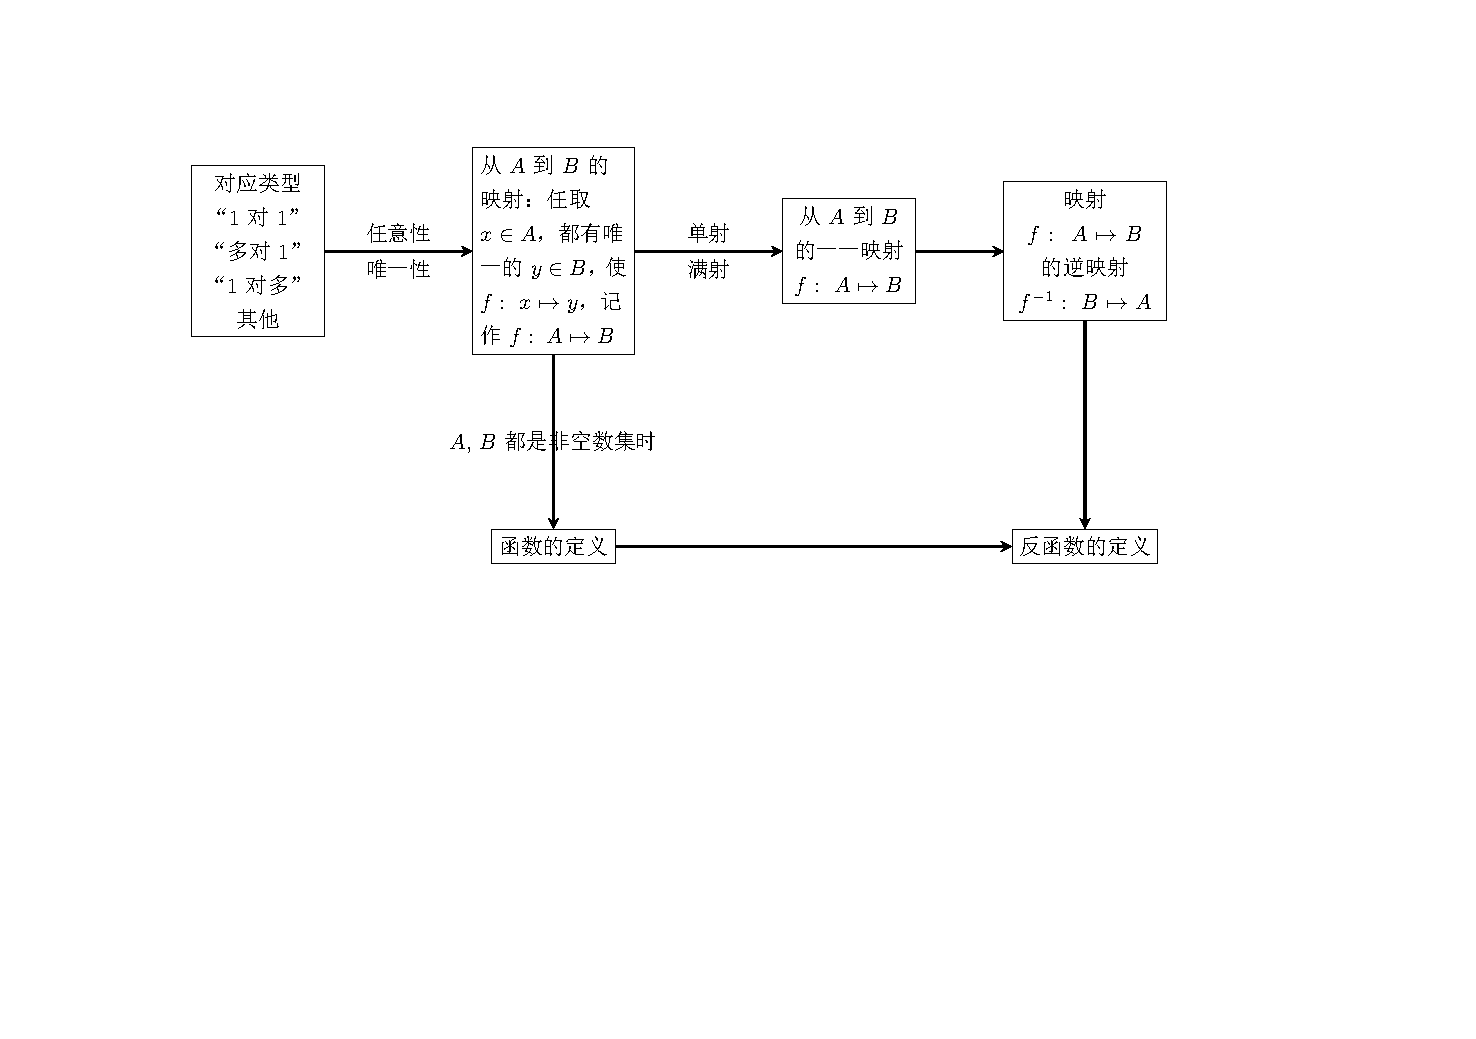
\includegraphics[scale=.75]{fig/fig2.pdf}
\end{center}

应注意:
\begin{enumerate}
    \item 每个定义都要正确叙述;
    \item 箭头指示了概念间的逻辑关系,应从理论发展的脉络上去理解。
\end{enumerate}

\subsubsection{函数概论的知识结构}

\begin{tikzpicture}[>=stealth]
\node[draw, rectangle](A) at (1,3+.75)[text width=1.5cm, align=center] {复合函数}; 
\node[draw, rectangle](B) at (1,0.75)[text width=1.5cm, align=center] {函数的\\定义}; 
\node[draw, rectangle](C) at (1,-3+.75)[text width=1.5cm, align=center] {函数\\表示法}; 
\draw[->, very thick](B)--(A);
\draw[->, very thick](B)--(C);

\node (E1) at (4,6)[right]{定义域(求法:归结为解不等式组)};
\node (E2) at (4,4.5)[right]{值域$\Bigg\{$};
\node (E21) at (5.25,5)[right]{值域的定义、求法};
\node (E22) at (5.25,4.5)[right]{特殊值(最大值、最小值)的求法};
\node (E23) at (5.25,4)[right]{给函数值的范围,求自变量的取值范围};
\node (E3) at (4,2.75)[right]{增减性$\Big\{$};
\node (E31) at (5.5,3)[right]{单调函数的定义、实质及判断};
\node (E32) at (5.5,2.5)[right]{单调区间的求法};
\node (E4) at (4,1.25)[right]{奇偶性$\Big\{$};
\node (E41) at (5.5,1.5)[right]{奇(偶)函数的定义、实质及判断};
\node (E42) at (5.5,1)[right]{奇偶性的应用};

\node (E5) at (4,.25)[right]{周期性(三角中待学)};

\node (E6) at (4,-1)[right]{画法$\Big\{$};
\node (E7) at (4,-2.5)[right]{看图认性质:函数性质与图象的一致性};
\node (E61) at (5.25,-.75)[right]{先讨论函数性质};
\node (E62) at (5.25,-1.25)[right]{再用描点法画图$\Big\{$};

\node (E71) at (8.5,-1)[right]{体现性质};
\node (E72) at (8.5,-1.5)[right]{标记特殊点};

\draw[decorate, very thick, decoration={brace, amplitude=10pt}](4,.25)--node[left=10pt]{性质}(4,6);

\draw[decorate, very thick, decoration={brace, amplitude=5pt}](4,-2.5)--node[left=7pt]{图象}(4,-1);

\draw[decorate, decoration={brace, amplitude=10pt}, very thick](2.5,-1.75)--(2.5,3);
\end{tikzpicture}

(这些内容的复习要结合有关小节进行)

\subsubsection{应掌握以下几点}
反函数存在的充要条件,反函数的求法,从函数的有关性质预测其反函数的性质(见2.6节)。


\subsubsection{图象的几种几何变换}
\begin{enumerate}
    \item $y=f(x)\longrightarrow y=f(x)+c$
   \hfill (纵向平移:上移$c$个单位)
    \item $y=f(x)\longrightarrow y=f(x+m)$
    \hfill   (横向平移:左移$m$个单位)
    \item $y=f(x)\longrightarrow y=-f(x)$
    \hfill   (关于$x$轴的对称变换)
    \item $y=f(x)\longrightarrow y=f(-x)$
    \hfill    (关于$y$轴的对称变换)
    \item $y=f(x)\longrightarrow y=|f(x)|$
    \item $y=f(x)\longrightarrow y=f(|x|)$
\end{enumerate}

\subsection{本章应着重掌握的数学思想}
\begin{enumerate}
\item 映射的思想:$\map{f}{A}{B},\quad \map{f}{x}{y},\; x\in A$.
\item 函数的思想:$y=f(x),\quad x\in A$.
\item 数、形结合的思想。
\item 函数、方程、不等式互相转化的思想。
\end{enumerate}

\section*{复习题二}
\begin{center}
    \bfseries A
\end{center}

\begin{enumerate}
    \item 设$M=\left\{a,b\right\}$, $N=\left\{x,y\right\}$, 从$M$到$N$的映射可以构造\blank
种,请用图示法表示这些映射。
\item 已知映射$\map{f}{A}{B}$, 其中$A=\{(x,y)\mid x\in \R,\; y\in \R\}$, 
$B=\{(\overline{x},\overline{y})\mid \overline{x}=x+y,\; \overline{y}=xy,\; x,y\in\R\}$,
$\map{f}{(x,y)}{(\overline{x},\overline{y})}$, $(x,y)\in A$, 则$(8,15)$的原象是\blank.

\item (选择题)使对应法则$\map{f}{x}{y}=x^2$成为从$X$到$Y$上的一
一映射的条件是(\quad ).
\begin{multicols}{2}
\begin{enumerate}[(A)]
    \item $X=Y=\R$
    \item $X=R,\; Y=\{\text{非负实数}\}$
    \item $X=\{\text{非负实数}\},\; Y=\R$
    \item $X=Y=\{\text{非负实数}\}$
\end{enumerate}
\end{multicols}

\item (选择题)$f( x) = \sqrt{x^{2}- 5x- 6}$ 的定义域是$F$, $g(x)=\sqrt{x-6}\cdot\sqrt{x+1}$ 的定义域是$G$, 则$F$ 与$G$ 的关系是(\quad).
\begin{multicols}{4}
    \begin{enumerate}[(A)]
        \item $F=G$
        \item $F\subset G$
        \item $F\supset G$
        \item $F\cap G=\emptyset$
    \end{enumerate}
    \end{multicols}
\item (选择题) 已知$0<a<1$, 设$x=a,\; y=2a,\;z=a^2$, 则$x,y,z$的大小关系是(\quad)
\begin{multicols}{4}
    \begin{enumerate}[(A)]
        \item $x<y<z$
        \item $z<y<x$
        \item $z<x<y$
        \item $x<z<y$
    \end{enumerate}
    \end{multicols}
\end{enumerate}

\begin{center}
    \bfseries B
\end{center}

\begin{enumerate}\setcounter{enumi}{5}
    \item (选择题)$f(x)=ax^2-6ax+1\; (a>0)$,则下列关系中正确的是(\quad)
\begin{multicols}{2}
    \begin{enumerate}[(A)]
        \item $f(\sqrt{2})>f(\sqrt{3})$
        \item $f\left(\frac{\pi}{2}\right)>f(\pi)$
        \item $f(\sqrt{5})<f(3)$
        \item $f(-1)<f(1)$
    \end{enumerate}
    \end{multicols}
\item (选择题)$f(x)=ax^3+cx+5$,已知$f(-3)=-3$,则$f(3)$等于(\quad)
\begin{multicols}{4}
    \begin{enumerate}[(A)]
        \item 3
        \item $-3$
        \item 2
        \item 13
    \end{enumerate}
    \end{multicols}
\item $f(x)$是偶函数,$g(x)$是奇函数,且$f(x)+g(x)=\frac1{x-1}$,
求$f(x)$与$g(x)$的表达式。

\item $f(x)=x^{3}+bx^{2}+cx$是奇函数,$g(x)=x^{2}-(c-2)x+5$是偶函数,则$b=\blank$, $c=\blank$.

\item 奇函数$F(x)$, 当$x<0$时,$F(x)=f(x)$, 则$F(x)$的完整表达式是\blank.

\item $y= \frac{1}{2} x+ a$与$y=3-bx$互为反函数,则$a=\blank$, $b=\blank$.
    
\item (选择题)$y=ax+b$与它的反函数是同一函数,则下列(\quad )中的数据是正确的。
\begin{multicols}{2}
    \begin{enumerate}[(A)]
        \item $a=1,\; b=0$
        \item $a=-1,\; b=0$
        \item $a=\pm 1,\; b=0$
        \item $a=1,\; b=0$;或$a=-1,\; b\in\R$
    \end{enumerate}
    \end{multicols}

\item (选择题)在函数$y= x- 1$, $y= x+ 1$,  $y= 2x- 1$, $y=2x+1$, $y=x^{2}$, $y=\sqrt{x}$, $y=x^{3}$, $y=\sqrt[{3}]{x}$中互为反
函数的有(\quad)
\begin{multicols}{4}
    \begin{enumerate}[(A)]
        \item 1对
        \item 2对
        \item 3对
        \item 4对
    \end{enumerate}
    \end{multicols}

\item $f(x)=\frac{x+1}{x-1}$, 则$f^{-1}(\sqrt{2})=\blank$.

\item $f(x)=3x-5$,则$f^{-1}[f(x)]=\blank$.

\item 将函数$y=\frac{1}{x}$的图象经过平移可以画出$y=\frac{x+3}{x+2}$的图
象,平移的步骤是\blank, \blank.
\end{enumerate}

\begin{center}
    \bfseries C
\end{center}

\begin{enumerate}\setcounter{enumi}{16}
\item 证明$f(x)=\frac x{x^2+1}$在$(-1,1)$上是增函数。

\item  函数$y=(x-1)^3+1$的图象的中心对称点的坐标是什么? 
\item 若$A=\{x\mid 10-3x-x^{2}\ge 0\}$, $B=\{x\mid m+1\leq x\leq 2m+1\}$, 
求实数$m$, 使$A\cap B\neq\emptyset$.
\item 奇函数$f(x)$在定义域$(-1,1)$上是单调 递增的,且
$f\left(1-a\right)+f\left(1-a^2\right)<0$, 求$a$的取值范围。
\end{enumerate}















 \chapter{幂函数、指数函数与对数函数}
上一章,通过“函数概论”的学习初步理解了研究函数的
基本途径和方法。本章将运用这些思想研究几类重要的初等
函数:幂函数、指数函数和对数函数。

\section{幂函数}
我们已经学过函数$y=x$, 
$y=x^2$
和
$y=x^{-1}$(即
$y=\frac{1}{x}$),
这些都是幂函数。

一般地,函数$y=x^{\alpha}$
($\alpha$是常数,
$\alpha\in\R$)
叫做幂函数,其
中$x$是自变量。

限于知识水平,本章只研究$\alpha$为有理数的情况,此时记
作
$y=x\; (n\in \Q)$.

先讨论幂函数
的定义域。

\begin{enumerate}[(1)]
    \item $n$为正整数时,$x^n$
的意义是$x=x\cdot x\cdots$(共有
$n$个$x$相乘)其定义域为
$D=(-\infty,+\infty)$;
\item $n$为正分数时,我们只研究$n$是既约分数$\frac{p}{q}$
的情况($p$、$q$是正整数,且
$q\ge 2$)这时$x^n$
的意义是$x^{\tfrac{p}{q}}=\sqrt[q]{x^p}$,函数定义域为使$\sqrt[q]{x^p}$有意义的实数$x$的集合,即当$q$
为奇数时,定义域
$D=(-\infty,+\infty)$,$q$
为偶数时($p$必为奇数),定
义域
$D=[0,+\infty)$
\item $n=0$时,$x^n=x^0$
,定义域
$D=(-\infty,0)\cup (0,+\infty)$;
\item $n$是负整数时,设
$n=-m,\; x^n=x^{-m}=\frac{1}{x^m},\; (m\in\N)$,
其定义域为$D=(-\infty,0)\cup (0,+\infty)$;
\item $n$是负分数时,
$n=-\frac{p}{q}$($p,q$为互质的正整数,
且$q\ge 2$)时,
\[x^n=\frac{1}{x^{\tfrac{p}{q}}}=\frac{1}{\sqrt[q]{x^p}}\]
当$q$为奇数时,定义域为
$D=(-\infty,0)\cup (0,+\infty)$; $q$为偶数时,
$D=(0,+\infty)$.

\end{enumerate}

总之,对于幂函数
$y=x^n\; (n\in\Q)$
来说,\textbf{使$x^n$
有意义的实
数$x$的集合就是它的定义域}。

\begin{example}
    说出下列幂函数的定义域:
\[y=x^0,\quad y=x^3,\quad y=x^{-2},\quad y=x^{\tfrac{1}{3}},\quad y=x^{\tfrac{1}{2}},\quad y=x^{-\tfrac{1}{2}}\]
\end{example}

\begin{solution}
$y=x^{0}$和$y=x^{-2}$的定义域为$(-\infty,0)\cup (0,+\infty)$;

$y=x^3$ 和 $y=x^{\tfrac13}$的定义域都是$(-\infty; +\infty)$;

$y=x^{\tfrac12}$的定义域为$[0, +\infty)$,\quad  $y=x^{-\tfrac12}$的定义域为$(0,+\infty)$。

\end{solution}

以下研究幂函数的图象和性质。

当$n=0$ 时,$y=x^{n}=1\; (x\neq0)$, 它的图象是与$y=1$ 重合
的一条直线 (除去点$(0,1)$).

下面着重研究$n\neq0$的情况。

当$n$是整数时。若$n$是奇数,可知$y=x^{n}$为奇函数,其图
象关于坐标原点对称,且图象在第一、三象限内;若$n$是偶
数,可知$y=x^n$
为偶函数,其图象关于$y$轴对称,且图象在第
一、二象限内;

当$n$为既约分数$\frac pq$($p$、$q$为整数,$q{\geq}2$, $p{\neq}0$)时:若 $q$、$p$ 均为奇数,可知函数$y=x^{\tfrac pq}$为奇函数,图象关 于 坐标原点对称,且图象在第一、三象限内;若$q$为奇数,$p$为偶数,可知函 数 $y=x^{\tfrac pq}$为偶函数,图象关于$y$轴对称,且图象在第一、二象限内;若$q$为偶数($p$ 只能是奇数), 可知函数$y=x^{\tfrac pq}$为非奇非偶函数,且图象只在第一象限内。

综上所述,只要把函数$y=x^n$ 在第一象限内的图象及其
特征搞清了,问题便迎刃而解。

\subsection{$n>0$时}
在同一坐标系内画出
$y=x^3$, $y=x^2$, $y=x$, $y=x^{\tfrac{1}{2}}$,$y=x^{\tfrac{1}{3}}$
在区间$[0,+\infty)$
上的图象如下:
\begin{figure}[htp]
    \centering
\begin{tikzpicture}[>=stealth, scale=2]
\draw[->](-.5,0)--(3,0)node[right]{$x$};
\draw[->](0,-.5)--(0,3)node[right]{$y$};
\draw[domain=0:2.5, smooth, very thick]plot(\x, \x)node[right]{$y=x$};
\draw[domain=0:1.5, smooth, very thick]plot(\x, \x^2)node[right]{$y=x^2$};
\draw[domain=0:1.35, smooth, very thick]plot(\x, \x^3)node[above right]{$y=x^3$};
\draw[domain=0:1.5, smooth, very thick]plot(\x^2,\x)node[above right]{$y=x^{\tfrac{1}{2}}$};
\draw[domain=0:1.35, smooth, very thick]plot(\x^3,\x)node[right]{$y=x^{\tfrac{1}{3}}$};
\draw[dashed](0,1)node[left]{1}--(1,1)--(1,0)node[below]{1};
\node[below left]{$O$};


\end{tikzpicture}
    \caption{}
\end{figure}

由图3.1可见,幂函数$y=x^n\; (n>0)$,当$x\in[0,+\infty)$时:
\begin{enumerate}[(1)]
\item 图象都过点$(0,0)$和$ (1, 1)$,
\item 都是单调增函数,
\item 对于$n_1>n_2>0$, 若$x_0\in ( 1, + \infty) $时,有$x_0^{n_1}>x_0^{n_2}$; 若$x_0\in(0,1)$ 时,$x_0^{n_1}<x_0^{n_2}$.
\end{enumerate}

\begin{example}
    讨论函数$y=x^{\tfrac{2}{3}}$
的定义域、值域、奇偶性,画出它的图象,并说明函数的单调区间。
\end{example}

\begin{solution}
函数$y=x^{\tfrac{2}{3}}=\sqrt[3]{x^2}$
,定义域为$(-\infty,+\infty)$,值域
为$[0,+\infty)$,由于
$f(-x)=\sqrt[3]{(-x)^2}=\sqrt[3]{x^2}=f(x)$
,所以
函数为偶函数。

图象关于$y$
轴对称。图象过$(0,0)$, $(1,1)$,
$(-1,1)$点:

由图3.2可知,幂函数
$y=x^{\tfrac{2}{3}}$
的单调增区间为$(0,+\infty)$
,单调减区间为$(-\infty,0)$.
\end{solution}





\begin{figure}[htp]
    \centering
\begin{minipage}{.6\textwidth}
\begin{tikzpicture}[>=stealth, scale=.6]
    \draw[->](-6,0)--(6,0)node[right]{$x$};
    \draw[->](0,-.5)--(0,5)node[right]{$y$};
    \draw[domain=0:5.75, smooth, very thick]plot(\x, {\x^(2/3)})node[above]{$y=x^{\tfrac{2}{3}}$};
    \draw[domain=0:5.75, smooth, very thick]plot(-\x, {\x^(2/3)});
\foreach \x in {-5,-3,-1,1,3,5}
{
    \draw(\x,0)node[below]{$\x$}--(\x,.2);
}
\draw[dashed](-1,1)--(1,1);
\node at (0,4)[right]{4};
\node at (0,2)[right]{2};
\draw[dashed](-2.828,2)--(2.828,2);
\draw[dashed](-1.732*3,3)--(1.732*3,3);
\draw(0,4)--(-.2,4);

\node[below right]{$O$};

\end{tikzpicture}
    \caption{}
\end{minipage}    \hfill
\begin{minipage}{.3\textwidth}
\begin{tikzpicture}[>=stealth]
    \draw[->](-.5,0)--(3,0)node[right]{$x$};
    \draw[->](0,-.5)--(0,3)node[right]{$y$};
    \draw[domain=0:2.5, smooth, very thick]plot(\x, {\x^(3/4)})node[above]{$y=x^{\tfrac{3}{4}}$};
\foreach \x in {1,2}
{
    \draw(\x,0)node[below]{\x}--(\x,.1);
    \draw(0,\x)node[left]{\x}--(.1,\x);
}
\node[below left]{$O$};

\end{tikzpicture}
\caption{}
\end{minipage}
\end{figure}






\begin{example}
画出函数$y=x^{\tfrac{3}{4}}$
的图象(草图),并说明其增减性。    
\end{example}

\begin{solution}
    应先讨论函数的性质,再画图象。

函数$y=x^{\tfrac{3}{4}}$的定义域为$[0,+\infty)$,
值域为$[0,+\infty)$,
为非奇非偶函数,图象在第一象限(含原点),见图3.3.

由图象可知,函数$y=x^{\tfrac{3}{4}}$
为单调增函数。
\end{solution}

\subsection{$n<0$时}
在同一坐标系内,画出
$y=x^{-2}$,$y=x^{-1}$和
$y=x^{-\tfrac{1}{2}}$
在区间$(0,+\infty)$
上的图象:

\begin{figure}[htp]
    \centering
\begin{tikzpicture}[>=stealth, scale=2]
    \draw[->](-.5,0)--(3.5,0)node[right]{$x$};
    \draw[->](0,-.5)--(0,3.5)node[right]{$y$};
    \draw[domain=0.55:2.5, smooth, very thick]plot(\x, {\x^(-2)})node[right]{$y=x^{-2}$};
    \draw[domain=0.3:2.5, smooth, very thick]plot(\x, {\x^(-1)})node[right]{$y=x^{-1}$};    
    \draw[domain=0.1:2.5, smooth, very thick]plot(\x, {\x^(-0.5)})node[above right]{$y=x^{-\tfrac{1}{2}}$};
\foreach \x in {1,2,3}
{
    \draw(\x,0)node[below]{\x}--(\x,.1);
    \draw(0,\x)node[left]{\x}--(.1,\x);
}
\node [below left]{$O$};
\draw[dashed](0,1)--(1,1)node[above right]{$(1,1)$}--(1,0);


\end{tikzpicture}
    \caption{}
\end{figure}

由图3.4可见,幂函数$y=x^n\; (n<0)$,当$x\in(0,+\infty)$时:
\begin{enumerate}[(1)]
    \item 图象都过点$(1,1)$;
    \item 都是单调减函数;
    \item 在第一象限内,图象向上与$y$轴无限地接近,向
    右与$x$轴无限地接近。称图象分别以$y$
    轴和$x$轴为\textbf{渐近线}。
    \item 对于$n_1<n_2<0$时, 若$x_0\in(1,+\infty)$时, 有$x_0^{n_1}<x_0^{n_2}$; 若$x_0\in(0,1)$时, $x_0^{n_1}>x_0^{n_2}$.
\end{enumerate}

\begin{example}
    在同一坐标系内,画出函数 $y= x^{-\tfrac{1}{2}}$, $ y= x^{\tfrac{1}{3}}$ 和
$y=x^{-2}$的图象。
\end{example}

\begin{solution}
    首先根据上述 $y=x^n$ 的图象和性质,作出这三个函
数在第一象限内的图象,再根据它们各自的奇偶性,分别作
出它们各自的完整的图象(图3.5)。
\end{solution}

\begin{figure}[htp]
    \centering
\begin{tikzpicture}[>=stealth, scale=1.5]
    \draw[->](-2.5,0)--(3,0)node[right]{$x$};
    \draw[->](0,-1.5)--(0,2.5)node[right]{$y$};
    \draw[domain=0.25:2.5, smooth, very thick]plot(\x, {\x^(-1/2)})node[above right]{$y=x^{-\tfrac12}$};
    \draw[domain=0:2.5, smooth, samples=100]plot(\x, {\x^(1/3)})node[above right]{$y=x^{\tfrac13}$};    
    \draw[domain=0.65:2.5, smooth, ultra thick]plot(\x, {\x^(-2)})node[right]{$y=x^{-2}$};
\foreach \x in {1,2}
{
    \draw(\x,0)node[below]{\x}--(\x,.1);
    \draw(0,\x)node[left]{\x}--(.1,\x);
}
\node [below left]{$O$};
\draw[dashed](0,-1)node[right]{$-1$}--(-1,-1)--(-1,0)node[below left]{$-1$}--(-1,1)--(1,1)--(1,0);

\draw[domain=0.65:2.5, smooth, ultra thick]plot(-\x, {\x^(-2)})node[above right]{$y=x^{-2}$};

\draw[domain=0:2.5, smooth, samples=100]plot(-\x, -{\x^(1/3)})node[below right]{$y=x^{\tfrac13}$};   

\end{tikzpicture}
    \caption{}
\end{figure}

\begin{note}
    本例题给出了作幂函数图象的步骤。
\begin{enumerate}[(1)]
    \item 先作出第一象限内的图象,
\item 若幂函数的定义域为$(0, +\infty)$(或$[0,+\infty)$),
作图已完成;若在$(-\infty,0)$或$(-\infty,0]$上有意义,则
只需根据函数的奇偶性,利用其图象的对称关系,作出第一象限图象关于原点或$y$轴的对称图象即可。
\end{enumerate}
\end{note}


\begin{example}
    比较下列各组数的大小:
 \begin{multicols}{2}
 \begin{enumerate}[(1)]
     \item $1.5^{\tfrac{2}{3}}$与$1.7^{\tfrac{2}{3}}$
     \item $\left(\sqrt{3}\right)^{\tfrac{5}{4}}$与$\left(\frac{5}{3}\right)^{\tfrac{5}{4}}$
     \item $3.14^{-\tfrac{4}{3}}$与$\pi^{-\tfrac{4}{3}}$
     \item $(-6.3)^{\tfrac{4}{3}}$与$(-6.4)^{\tfrac{4}{3}}$
     \item $\left(-\sqrt{2}\right)^{-\tfrac{3}{5}}$与$\left(-\sqrt{3}\right)^{-\tfrac{3}{5}}$
 \end{enumerate}
 \end{multicols}
 \end{example}
 
 \begin{analyze}
     各题中的两个值都是“同指数”的幂,因此可看作是同一个幂函数的两个不同的函数值。从而可据幂函数的单调性做出判断.
 \end{analyze}
 
 \begin{solution}
 \begin{enumerate}[(1)]
     \item 由于幂函数$y=x^{\tfrac{2}{3}}\; (x>0)$单调递增,且$1.5<1.7$
 
     $\therefore\quad 1.5^{\tfrac{2}{3}} < 1.7^{\tfrac{2}{3}}$
 \item 由于幂函数$y=x^{\tfrac{5}{4}}\; (x>0)$单调递增,且$\sqrt{3}>\frac{5}{3}$
 
 $\therefore\quad \left(\sqrt{3}\right)^{\tfrac{5}{4}} > \left(\frac{5}{3}\right)^{\tfrac{5}{4}}$
 \item 由于幂函数$y=x^{-\tfrac{4}{3}}\; (x>0)$单调递减,且$3.14<\pi$
 
 $\therefore\quad 3.14^{-\tfrac{4}{3}} < \pi^{-\tfrac{4}{3}}$
 \item 由于幂函数$y=x^{\tfrac{4}{3}}$是偶函数
 
 $\therefore\quad f(-x)=f(x)$,由此:
 \[(-6.3)^{\tfrac{4}{3}}=6.3^{\tfrac{4}{3}},\qquad (-6.4)^{\tfrac{4}{3}}=6.4^{\tfrac{4}{3}}\]
 而$y=x^{\tfrac{4}{3}}\; (x>0)$单调递增,且$6.3<6.4$,
 
 $\therefore\quad 6.3^{\tfrac{4}{3}} < 6.4^{\tfrac{4}{3}}$,从而:$(-6.3)^{\tfrac{4}{3}} < (-6.4)^{\tfrac{4}{3}}$
 \item 由于幂函数$y=x^{-\tfrac{3}{5}}$是个奇函数
 
 $\therefore\quad f(-x)=-f(x)$,由此
 \[\left(-\sqrt{2}\right)^{-\tfrac{3}{5}}=-\left(\sqrt{2}\right)^{-\tfrac{3}{5}},\qquad \left(-\sqrt{3}\right)^{-\tfrac{3}{5}}=-\left(\sqrt{3}\right)^{-\tfrac{3}{5}}\]
 
 而$y=x^{-\tfrac{3}{5}}\; (x>0)$单调递减,且$\sqrt{2}<\sqrt{3}$
 
 $\therefore\quad \left(\sqrt{2}\right)^{-\tfrac{3}{5}}>\left(\sqrt{3}\right)^{-\tfrac{3}{5}}\Longrightarrow -\left(\sqrt{2}\right)^{-\tfrac{3}{5}}<-\left(\sqrt{3}\right)^{-\tfrac{3}{5}}$
 
 $\therefore\quad \left(-\sqrt{2}\right)^{-\tfrac{3}{5}}< \left(-\sqrt{3}\right)^{-\tfrac{3}{5}}$
 \end{enumerate}
 \end{solution}
 
 \begin{note}
 (4)、(5)两题中,我们是利用幂函数的奇、偶
     性,先把底为负数的幂转化为正数的幂解决问题。当然,若直接利用$x<0$上的幂函数的单调性解决问题也是可行的。
 \end{note}
 
 \begin{example}
 求函数$y=(x-3)^{-2}$的定义域,并讨论其增减性。  
 \end{example}
 
 \begin{solution}
 \[y=(x-3)^{-2}=\frac{1}{(x-3)^2}\]
 定义域为$D=(-\infty,3)\cup (3,+\infty)$.
 
 因为$y=(x-3)^{-2}$可看作是由函数$y=x^{-2}$的图象向右平移3个单位后的结果,所以,当$x\in (-\infty,3)$时,函数单调递增;而当$x\in(3,+\infty)$时,函数单调递减。
 \end{solution}
 
 \begin{note}
     把所要研究的问题\underline{化归}为熟知的事实,这是数学中处理问题的常用思维方式。
 \end{note}
 
 
 \section*{习题一}
 \begin{center}
     \bfseries A
 \end{center}
 
 \begin{enumerate}
     \item 写出下列函数的定义域,值域,并讨论其奇偶性:
 \begin{multicols}{2}
 \begin{enumerate}[(1)]
     \item $y=x^{-2}$
     \item $y=x^{\tfrac{5}{7}}$
     \item $y=x^{\tfrac{4}{5}}$
     \item $y=x^{\tfrac{5}{6}}$
     \item $y=x^{-\tfrac{3}{2}}$
     \item $y=x^{-\tfrac{4}{5}}$
 \end{enumerate}
 \end{multicols}
     \item 写出下列函数的定义域,并讨论其奇偶性:
 \begin{multicols}{2}
 \begin{enumerate}[(1)]
     \item $f_1(x)=x^2+x^{-2}$
     \item $f_2(x)=x+3x^{\tfrac{2}{3}}$
     \item $f_3(x)=2x+\sqrt[3]{x}$
     \item $f_4(x)=2x^{-4}-3x^{-2}$
 \end{enumerate}    
 \end{multicols}
 \item 讨论下列函数的定义域、值域、奇偶性,并画出函数的图象:
 \begin{multicols}{3}
 \begin{enumerate}[(1)]
     \item $y=x^{\tfrac{3}{4}}$
     \item $y=x^{-\tfrac{2}{3}}$
     \item $y=x^{-\tfrac{1}{2}}$
 \end{enumerate}
 \end{multicols}
 
 \item 在同一坐标系内,画出下列各题中的两个函数的图象,并加以比较:
 \begin{multicols}{2}
 \begin{enumerate}[(1)]
     \item $y=x^3,\quad y=x^4$
     \item $y=x^{-3},\quad y=x^{-4}$
 \end{enumerate}
 \end{multicols}
 
 \item 比较下列各题中两个值的大小:
 \begin{multicols}{2}
 \begin{enumerate}[(1)]
     \item $2.3^{\tfrac{3}{4}}$与$2.4^{\tfrac{3}{4}}$
     \item $0.7^{\tfrac{2}{3}}$与$0.8^{\tfrac{2}{3}}$
     \item $\left(\sqrt{2}\right)^{-\tfrac{3}{2}}$与$\left(\sqrt{3}\right)^{-\tfrac{3}{2}}$
     \item $1.1^{-\tfrac{1}{2}}$与$0.9^{-\tfrac{1}{2}}$
     \item $\left(\frac{3}{7}\right)^{-\tfrac{4}{3}}$与$\left(\frac{5}{8}\right)^{-\tfrac{4}{3}}$
     \item $(-\pi)^{\tfrac{2}{3}}$与$(-3.1)^{\tfrac{2}{3}}$
     \item $\left(-\frac{10}{11}\right)^{\tfrac{3}{5}}$与$\left(-\frac{11}{12}\right)^{\tfrac{3}{5}}$
 \end{enumerate}
 \end{multicols}
 
 \end{enumerate}
 
 \begin{center}
     \bfseries B
 \end{center}
 
 \begin{enumerate}\setcounter{enumi}{5}
     \item 求函数$y=(x+2)^{-2}$的定义域、值域,画出它的图象,并写出它的单调区间。
 \item     把幂函数$y=x^r\; (r\in\Q)$的图象经过怎样平移,可得到$y=(x+m)^r+n\; (mn\ne 0)$的图象?
 \item     把幂函数$y=\frac{1}{x}$的图象经过怎样平移,可得到
     $y=\frac{3x+7}{x+2}$的图象?
 \end{enumerate}
 
 
 \begin{center}
     \bfseries C
 \end{center}
 
 \begin{enumerate}\setcounter{enumi}{8}
 \item \begin{enumerate}[(1)]
     \item 由$y=x$的图象,经过取倒数变换画出$y=\frac{1}{x}$的图象(草图)。
     \item 由$y=x^3$的图象,经过取倒数变换画出$y=x^{-3}$的图象(草图)。
     \item 由$y=x^{\tfrac{1}{2}}$的图象,经过取倒数变换可以画出哪个函数的图象?试画一下。
 \end{enumerate}
 \end{enumerate}
 
 \section{指数函数}
 \subsection{指数函数的概念}
     
 在幂函数$y=x^{\alpha}$(常数$\alpha\in\R$)中,底数是自变量,指数$\alpha$是常数,即“底数变、指数不变”。若令“底数不变、指数变”,如$y=2^x,\; y=10^x\; y=\left(\frac{1}{2}\right)^x$等等,则称$y$是$x$的指数函数。
 
 一般地,函数$y=a^x$ $(0<a\ne 1)$叫\textbf{指数函数},自变量为$x$。其中$a$是不等于1的正常数\footnote{当$a>0$时,若$x$是无理数,$a^x$是一个确定的实数;对于无理指数幂,过去学过的有理指数幂的性质和运算法则都适用,有关概念与定理证明在本书中从略.
 
 若$a=1$, $y=1^x$极其简单,没有研究的价值.
 
 若$a<0$, $y=a^x$不是对任意实数$x$都有意义,并且极为复杂,因此我们也不去研究它.}.函数的定义域$D=\R$.
 
 \subsection*{指数函数的实例}
 \begin{example}
     某种细胞分裂时,由1个分裂为2个,2个分裂为4个,……,一个这样的细胞分裂$x$次后,得到的个数$y$与$x$的函数关系是
 \[y=2^x,\qquad x\in\N\]
 这是一个指数型函数。
 \end{example}
 
 \begin{example}
     某速生林区现有森林资源$M$立方米。如果平均年增长率为10\%,计算一年后,两年后,三年后,……,$x$年后各有森林资源多少立方米。
 \end{example}
 
 \begin{figure}[htp]
     \centering
 \begin{tikzpicture}[xscale=.7, yscale=.9]
 \draw(0,0)--(12,0);
 \draw[fill=gray](1,0)node[below]{基数} rectangle (1.2,4)node[above]{$M$};
 \draw[fill=gray](4,0)node[below]{一年后} rectangle (4.2,4.4)node[above]{$y_1$};
 \draw[fill=gray](7,0)node[below]{两年后} rectangle (7.2,4.84)node[above]{$y_2$};
 \draw[fill=gray](10,0)node[below]{三年后} rectangle (10.2,4.84*1.1)node[above]{$y_3$};
 \draw[dashed](1,4)--(4,4);
 \draw[dashed](4,4.4)--(7,4.4);
 \draw[dashed](7,4.84)--(10,4.84);
 \draw[decorate, decoration=brace, xshift=-2pt](4,0)--node[left]{$M$}(4,4);
 \draw[decorate, decoration=brace, xshift=-2pt](7,0)--node[left]{$y_1$}(7,4.4);
 \draw[decorate, decoration=brace, xshift=-2pt](10,0)--node[left]{$y_2$}(10,4.84);
 \draw[decorate, decoration=brace, xshift=2pt](4.2,4.4)--node[right]{$M\times 10\%$}(4.2,4);
 \draw[decorate, decoration=brace, xshift=2pt](7.2,4.84)--node[right]{$y_1\times 10\%$}(7.2,4.4);
 \draw[decorate, decoration=brace, xshift=2pt](10.2,4.84*1.1)--node[right]{$y_2\times 10\%$}(10.2,4.84);
 
 
 
 
 \end{tikzpicture}
     \caption{}
 \end{figure}
 
 
 
 \begin{solution}
 设$x$年后林区森林资源为$y_x$立方米(图3.6),则
 \[\begin{split}
     y_1&=M+M\times 10\%=M(1+10\%)\\
     y_2&=y_1+y_1\times 10\%=y_1(1+10\%)=M(1+10\%)^2\\
     y_3&=y_2+y_2\times 10\%=y_2(1+10\%)=M(1+10\%)^3\\
 \cdots&\cdots\\
     y_x&=M(1+10\%)^x\\
 \end{split}\]
 其中表达式$(1+10\%)^x=1.1^x$也是一个指数型函数。
 \end{solution}
 
 
 \begin{ex}
     (填空)某厂去年12月份产值为32万元。今年1月份比上一个月份增产8\%.2月份比1月份减产5\%.3月份比2月份又减产7\%.4月份比3月份增产10\%。那么4月份的产值是\blank 万元。
 \end{ex}
 
 \subsection{指数函数的图象}
 
 先画出一些指数函数的图象,例如,画出$y=2^x$, 
 $y=\left(\frac{1}{2}\right)^x$, $y=10^x$的图象。
 
 列表,用描点法画图(图3.7)
 \begin{table}[htp]
     \centering
     \caption{}    
 \begin{tabular}{c|ccccccccc}
 \hline
         $x$ & $\cdots $&$-3$&$-2$&$-1$&0&1&2&3&$\cdots$\\
 \hline
 $y=2^x$ & $\cdots$&$\frac{1}{8}$ &$\frac{1}{4}$& $\frac{1}{2}$& 1&2&4&8&$\cdots$\\
 $y=\left(\frac{1}{2}\right)^x$ &$\cdots$&8&4&2&1&$\frac{1}{2}$&$\frac{1}{4}$&$\frac{1}{8}$&$\cdots$\\
 \hline
     \end{tabular}
 
 \begin{tabular}{c|ccccccc}
 \hline
 $x$&$\cdots$&$-1$&$-\frac{1}{2}$&0&$\frac{1}{2}$&1&$\cdots$\\
 \hline
 $y=10^x$&$\cdots$0.1&0.32&1&3.16&10&$\cdots$\\
 \hline
 \end{tabular}
 \end{table}
 
 \begin{figure}[htp]
     \centering
 \begin{tikzpicture}[>=stealth, scale=.6]
 \draw[->](-5,0)--(5,0)node[right]{$x$};
 \draw[->](0,-2)--(0,11)node[right]{$y$};
 \foreach \x in {-3,-2,-1,1,2,3}
 {
     \draw(\x,0)node[below]{$\x$}--(\x,.2);
 }
 \foreach \x in{1,2,3,...,10}
 {
     \draw(0,\x)node[left]{$\x$}--(.2,\x);
 }
 \draw[domain=-4:1, smooth, very thick]plot(\x, 10^\x)node[right]{$y=10^x$};
 \draw[domain=-3:4, smooth, very thick]plot(\x, 0.5^\x);
 \node [below right]{$O$};
 \node at (-3,8)[above]{$y=\left(\frac{1}{2}\right)^x$};
 \draw[domain=-4:3, smooth, very thick]plot(\x, 2^\x)node[right]{$y=2^x$};
 
 
 \end{tikzpicture}
     \caption{}
 \end{figure}
 
 
 我们看到这些图象的共同点是:
 
 图象都在$x$轴上方,即对任何$x\in\R$,都有$y>0$;图象都通过$(0,1)$点,即当$x=0$时,恒有$y=a^0=1\; (0<a\ne 1)$,当$a>1$时,曲线以$x$轴负方向为渐近线,且当$x$增加时,曲线是上升的(即$y$是$\R$上的增函数);当$0<a<1$时,曲线以$x$轴正方向为渐近线,且当$x$增加时,曲线是下降的(即$y$是$\R$上的减函数)。
 
 我们还看到:$y=2^x$与$y=\left(\frac{1}{2}\right)^x$这样两个函数的图象关于$y$轴对称(这一点你能从理论上证明吗?)。
 
 \subsection{指数函数$y=a^x\; (0<a\ne 1)$的性质}
 列表如下:
 \begin{table}[htp]
     \caption{}
     \centering
 \begin{tabular}{c|cc}
     \hline
 $y=a^x$ & $a>1$&$0<a<1$        \\
 \hline
 定义域 & $\R$ & $\R$\\
 值域 & $(0,+\infty)$& $(0,+\infty)$\\
 &\multicolumn{2}{c}{任一正数$m$都能写成指数形式$m=a^x$}\\
 单调性& $y$是$\R$上的增函数& $y$是$\R$上的减函数\\
 & $a^x=\begin{cases}
     <1,& x<0\\
     =1,& x=0\\
     >1,& x>0
 \end{cases}$  & $a^x=\begin{cases}
     >1,& x<0\\
     =1,& x=0\\
     <1,& x>0
 \end{cases}$\\
 关键点&\multicolumn{2}{c}{$(0,1),\quad (1,a),\quad \left(-1,\frac{1}{a}\right)$}\\
 底数对图象的影响&\multicolumn{2}{c}{$y=a^x$与$y=\left(\frac{1}{a}\right)^x$的图象关于$y$轴对称}\\
 \hline
 \end{tabular}
 \end{table}
 
 \begin{center}
 \begin{tikzpicture}[>=stealth]
 \begin{scope}
 \draw[->](-2,0)--(2,0)node[right]{$x$};
 \draw[->](0,-1)--(0,4)node[right]{$y$};
 \node [below left]{$O$};
 
 \foreach \x in {1,2,3}
 {
     \draw(0,\x)--(-.1,\x)node[left]{$\x$};
 }
 \foreach \x in{-1,1}
 {
     \draw(\x,0)--(\x,-.1)node[below]{$\x$};
 }
 \draw[domain=-1.5:1.5, smooth, very thick]plot(\x, 2^\x)node[above]{$y=a^x$};
 \node at (1,1)[right]{$(a>1)$};
 \end{scope}
 \begin{scope}[xshift=6cm]
     \draw[->](-2,0)--(2,0)node[right]{$x$};
 \draw[->](0,-1)--(0,4)node[right]{$y$};
 \foreach \x in {1,2,3}
 {
     \draw(0,\x)--(-.1,\x)node[left]{$\x$};
 }
 \foreach \x in{-1,1}
 {
     \draw(\x,0)--(\x,-.1)node[below]{$\x$};
 }
 \draw[domain=1.5:-1.5, smooth, very thick]plot(\x, 0.5^\x)node[above]{$y=a^x$};
 \node at (-.5,1)[left]{$(0<a<1)$};
 \node [below left]{$O$};
 
 \end{scope}
 \end{tikzpicture}
 \end{center}
 
 \begin{note}
 \begin{enumerate}
     \item 在分析问题时,常常需要画出较正确的指数函数的
 草图。一般至少取三个点$(1,a)$、$(0,1)$与$\left(-1,\frac{1}{a}\right)$并且注意$x$轴是渐近线;
 \item 因为$y=a^x$的值域是$(0,+\infty)$,且在$\R$上$y$是$x$的单调函数,所以任意$m\in (0,\infty)$,都应找到唯一的$x_0$与之对应,即$m=a^{x_0}$。这就是说,\textbf{任一正数$m$都能写成指数形式};
 \item $a>1$时,由于$y=a^x$是$a$的增函数,且过$(0,1)$点,立刻可得
 \[a^x \begin{cases}
     <1,& x<0\\
     =1,& x=0\\
     >1,& x>1
 \end{cases}\]
 (从图象上看,这一点十分清楚!)
 
 这是一组十分重要的不等关系。连同$0<a<1$时的不等关系与之类似(见表3.2);
 \item 若$f(x)=a^x$,则$f(-x)=a^{-x}=\left(\frac{1}{a}\right)^x$,这说明由$y=a^x$的图象作关于$y$轴的对称变换立刻可得到$y=\left(\frac{1}{a}\right)^x$的图
 象。所以$y=a^x$与$y=\left(\frac{1}{a}\right)^x$的图象关于$y$轴对称。
 \end{enumerate}
 \end{note}
 
 \begin{example}
     一种放射性物质不断蜕变为其他物质,每过一年剩留质量约为原来的84\%,写出剩留质量$y$与经过的时间$x$(年)的关系式,并通过其函数图象求出约经过多少年剩留质量恰为原来的一半(结果保留一个有效数字).
 \end{example}
 
 \begin{solution}
    设最初的质量为1。经过1年,剩留质量是$y_1=1\times 4\%=0.84$,经过2年,剩留质量$y_2=0.84\times 84\%=0.84^2$, 经过$x$年,剩留质量$y_x=0.84^x\; (x\ge 0)$,这是一个指数函数,据此列表:
 \begin{center}
     \begin{tabular}{ccccccccc}
 \hline
 $x$&0&1&2&3&4&5&6&$\cdots$\\
 \hline
 $y$&1&0.84&0.71&0.59&0.50&0.42&0.35&$\cdots$ \\
 \hline
     \end{tabular}
 \end{center}
 用描点法画出函数的图象(图3.8)。因为这是一个减函数的图象[底数$a\in(0,1)$],从图上看出:要使$y=0.5$, $x=4$.
 \begin{figure}[htp]
     \centering
 \begin{tikzpicture}[yscale=4, xscale=.6,>=stealth]
 \draw[->](-1,0)--(7,0)node[right]{$x$};
 \draw[->](0,-.15)--(0,1.1)node[left]{$y$};
 \foreach \x in {1,2,...,6}
 {
     \draw(\x,0)node[below]{$\x$}--(\x,.03);
 }
 \foreach \x in {0.2,0.4,0.6,0.8}
 {
     \draw(0,\x)node[left]{$\x$}--(.2,\x);
 }
 \draw[domain=0:6, smooth, very thick]plot(\x, 0.84^\x);
 \node [below left]{$O$};
 \draw[dashed](0,.5)--(6,.5);
 \draw[dashed](4,0)--(4,.5);
 
 \end{tikzpicture}
     \caption{}
 \end{figure}
 
 答:约过4年,剩留质量为原来之半。
 \end{solution}
 
 \begin{ex}
 由$y=2^x$的图象,你能简捷地作出下列函数的图象吗?
 \begin{multicols}{2}
 \begin{enumerate}[(1)]
     \item $y=2^{x+3}-1$
     \item $y=2^{x-3}+1$
     \item $y=4\cdot 2^x$
     \item $y=\left(\frac{1}{2}\right)^x$
     \item $y=-2^{x}$
     \item $y=2^{|x|}$
 \end{enumerate}
 \end{multicols}
 \end{ex}
 
 \begin{analyze}
     运用图象几何变换的方法(见2.9节)能简捷地作出这些函数的图象。
 \end{analyze}
 
 \begin{example}
     求出$y=2^{x+3}-1$与$y=2^{|x|}$的定义域、值域和单调区间。
 \end{example}
 
 \begin{solution}
 \begin{enumerate}[(1)]
     \item 由$y=2^x$的图象左移3个单位,再下移1个
     单位,可得到$y=2^{x+3}-1$的图象(图3.9).从而可知,$D=\R$,值域是$(-1,+\infty)$, 它的增区间是$(-\infty,+\infty)$。
     \item 因为$y=2^{|x|}$是偶函数,当$x\ge 0$时与$y=2^x\; (x\ge 0)$的图象重合。由对称性可作出$x<0$时的图象(图3.10).所以,$y=2^{|x|}$的定义域是$\R$,值域是$[1,+\infty)$, $(-\infty,0]$是减区间,$[0,+\infty)$是增区间。
 \end{enumerate}
 \begin{figure}[htp]
     \centering
 \begin{minipage}{.45\textwidth}
     \begin{tikzpicture}[>=stealth, scale=.7]
 \draw[->](-4,0)--(3,0)node[right]{$x$};
 \draw[->](0,-1)--(0,4)node[right]{$y$};
 \draw[domain=-4:-1, smooth, very thick]plot(\x, 8*2^\x -1)node[above left]{$y=2^{x+3}-1$};
 \draw[domain=-3:1.7, smooth, dashed, very thick]plot(\x, 2^\x)node[right]{$y=2^{x}$};        
 \node [below right]{$O$};
 \foreach \x in {-3,-2,-1,1,2}
 {
     \draw(\x,0)node[below]{$\x$}--(\x,.1);
 }
 \foreach \x in{1,2,3}
 {
     \draw(0,\x)--(.1,\x)node[right]{$\x$};
 }
 
     \end{tikzpicture}
 \caption{}    
 \end{minipage}
 \hfill
 \begin{minipage}{.45\textwidth}
 \begin{tikzpicture}[>=stealth, scale=.6]
     \draw[->](-2.5,0)--(3,0)node[right]{$x$};
     \draw[->](0,-1)--(0,5)node[right]{$y$};
     \draw[domain=0:2, smooth, very thick]plot(\x, 2^\x)node[above]{$y=2^{|x|}$};
     \draw[domain=0:2, smooth, very thick]plot(-\x, 2^\x);
     \draw[domain=-2:0, smooth, dashed, very thick]plot(\x, 2^\x);
     \node [below right]{$O$};
     \foreach \x in {-2,-1,1,2}
     {
         \draw(\x,0)node[below]{$\x$}--(\x,.1);
     }
     \foreach \x in{1,2,3,4}
     {
         \draw(0,\x)--(.1,\x)node[right]{$\x$};
     }
 \end{tikzpicture}
     \caption{}    
     \end{minipage}
 \end{figure}
 
 
 \end{solution}
 
 \begin{example}
     比较下列每题中两个数的大小。
 \begin{multicols}{2}
 \begin{enumerate}[(1)]
     \item $0.6^{-2.1}$与$0.8^{- 2.1}$
     \item $( 2\sqrt 2) ^{\tfrac 13}$与$\left(\frac7{18}\right)^{-\tfrac{1}{3}}$
     \item $1.7^{-2.5}$与$1.7^{-2.1}$
     \item $0.9^{0.1}$与$0.9^{0.2}$
 \end{enumerate}
 \end{multicols}
 \end{example}
 
 \begin{analyze}
     (1)、(2)题是“同指数”的幂,可利用幂函数
 的单调性比大小,(3)、(4)题是“同底数”的幂,可利用指数函数的单调性比大小。
 \end{analyze}
 
 \begin{solution}
 \begin{enumerate}[(1)]
     \item $\because \quad $幂函数 $y=x^{-2.1}\; (x>0)$单调递减,且$0.6<0.8$,
     
 $\therefore\quad 0.6^{-2.1}>0.8^{-2.1}$    
 
 \item $\because\quad $幂函数$y=x^{\tfrac13}\; (x>0)$单调递增,且
 $2\sqrt{2}<\frac{18}{7}$,
 
 $\therefore\quad ( 2\sqrt 2) ^{\tfrac 13}<\left(\frac7{18}\right)^{-\tfrac{1}{3}}$
 
 \item $\because \quad $指数函数$y=1.7^x$单调递增,且$-2.5<-2.1$,
 
 $\therefore\quad 1.7^{-2.5}<1.7^{-2.1}$
 
 \item $\because \quad $指数函数$y=0.9^x$单调递减,且$0.1<0.2$,
 
 $\therefore\quad 0.9^{0.1}>0.9^{0.2}$
 \end{enumerate}
 \end{solution}
 
 \begin{example}
     比较下列各题中两个数的大小:
 \begin{multicols}{2}
 \begin{enumerate}[(1)]
     \item $2.6^{3.2}$与$\left ( \frac 1{\sqrt {5}}\right ) ^{- 3.2} $, 
     \item $1.8^{3.4}$与$3^{1.7}$,
     \item $\left(\frac7{10}\right)^{-0.81}$与$\left(1\frac37\right)^{0.92}$,
     \item $1.7^{0.3}$与$0.9^{3.1}$
 \end{enumerate}
 \end{multicols}
 \end{example}
 
 \begin{analyze}
     这些幂既不同指数,又不同底数,但除(4)以
 外,有的能化成“同底”,有的能化成“同指”。
 \end{analyze}
 
 \begin{solution}
 \begin{enumerate}[(1)]
     \item $\because\quad \left(\frac{1}{\sqrt{5}}\right)^{-3.2}=(\sqrt{5})^{3.2}$,幂函数$y=x^{3.2}\; (x>0)$单调递增,且$2.6>\sqrt{5}$,
     
 $\therefore\quad 2.6^{3.2}>\left ({\sqrt {5}}\right ) ^{3.2}\Longrightarrow 2.6^{3.2}>\left ( \frac 1{\sqrt {5}}\right ) ^{- 3.2}$
 
 \item $\because\quad 3^{1.7}=\left(\sqrt{3}\right)^{3.4}$,幂函数$y=x^{3.4}\; (x>0)$单调递增,且$1.8>\sqrt{3}$,
 
 $\therefore\quad 1.8^{3.4}>\left ({\sqrt {3}}\right ) ^{3.4}\Longrightarrow 1.8^{3.4}>3^{1.7}$.
 
 \item $\because\quad \left(1\frac{3}{7}\right)^{0.92}=\left(\frac{7}{10}\right)^{-0.92}$,指数函数$y=\left(\frac{7}{10}\right)^x$单调递减,且$-0.81>-0.92$,
 
 $\therefore\quad \left(\frac{7}{10}\right)^{-0.81}<\left(\frac{7}{10}\right)^{-0.92}\Longrightarrow \left(\frac{7}{10}\right)^{-0.81}<\left(1\frac{3}{7}\right)^{0.92}$.
 
 \item 分析:因为$1.7^{0.3}$与$0.9^{3.1}$既不“同底”,也不“同
 指”,又化不成“同底”或“同指”。所以,不能直接利用某个指数函数(或幂函数)的单调性比大小。现在考虑能否在这两个数值之间寻找一个中间值,使它比其中一个数大,而比另外一个数小.
 
 \textbf{方法1:} 由指数函数的单调性,有
 \[1.7^{0.3}>1.7^0=1,\qquad 0.9^{3.1}<0.9^0=1\]
 即:$1.7^{0.3}>1,\quad 0.9^{3.1}<1$\hfill (图3.11)
 
 $\therefore\quad 1.7^{0.3}>0.9^{3.1}$.
 
 \textbf{方法2:} 由幂函数的单调性,有
 \[1.7^{0.3}>1^{0.3}=1,\qquad 0.9^{3.1}<1^{3.1}=1\]
 即
 $1.7^{0.3}>0.9^{3.1}$\hfill (图3.12)
 \end{enumerate}
 \end{solution}
 
 \begin{figure}[htp]
     \centering
 \begin{minipage}{.45\textwidth}
 \begin{tikzpicture}[scale=.8, >=stealth]
    \draw[->](-2,0)--(4,0)node[right]{$x$};
 \draw[->](0,-1)--(0,4)node[right]{$y$};
 \node [below left]{$O$};
 \draw[domain=-1.5:2.5, smooth, very thick]plot(\x, 1.7^\x)node[right]{$y=1.7^x$};
 \draw[domain=-2:3.5, smooth, very thick]plot(\x, 0.9^\x)node[above]{$y=0.9^x$}; 
 \draw[dashed](0.3,0)--(0.3,1.7^0.3);
 \draw[dashed](3.1,0)--(3.1,0.9^3.1);
 \foreach \x in {1,2,3}
 {
     \draw(\x,0)node[below]{\x}--(\x,.1);
 }
 
 \end{tikzpicture}
 \caption{}
 \end{minipage}\hfill
 \begin{minipage}{.45\textwidth}
 \begin{tikzpicture}[scale=1.2, >=stealth]
     \draw[->](-.5,0)--(3,0)node[right]{$x$};
 \draw[->](0,-.5)--(0,3)node[right]{$y$};
 \node [below left]{$O$};    
 \draw[domain=0:1.3, smooth, very thick, samples=100]plot(\x, \x^3.1)node[above right]{$y=x^{3.1}\; (x>0)$};
 \draw[domain=0:2.7, smooth, very thick, samples=1000]plot(\x, \x^0.3)node[above]{$y=x^{0.3}\; (x>0)$}; 
 \draw[dashed](1,0)node[below]{1}--(1,1)node[below right]{$(1,1)$};
 \draw[dashed](0,1)--(.1,1)node[right]{1};
 \draw[dashed](1.7,0)node[below]{1.7}--(1.7,1.7^0.3);
 \draw[dashed](0.9,0)--(0.9,0.9^3.1);
 
 
 \end{tikzpicture}
 \caption{}
 \end{minipage}
 \end{figure}
 
 
 
 
 \begin{note}
 (1)、(2)、(3)题是把要比大小的幂“转化”为同底幂或同指数幂加以处理。第(4)题方法的实质是在要比大小的两个幂之间搭一个桥(找一个中间值),间接达到比大小的目的,这种方法不妨称为中间值法(也是一种有用的思考方法).本题在寻找中间值的过程中,利用了指数函数的关键点$(0,1)$与幂函数的关键点$(1,1)$附近的函数的性质.
 \end{note}
 
 \begin{example}
 解不等式:\begin{multicols}{2}    
 \begin{enumerate}[(1)]
     \item $a^{2x^2-7x+3}>1\; (a>1)$
     \item $a^{2x^2-3x+1}>a^{x^2+2x-5}\; (0<a<1)$
 \end{enumerate}
 \end{multicols}
 \end{example}
 
 \begin{solution}
 \begin{enumerate}[(1)]
     \item 原不等式可写成
 $$a^{2x^2-7x+3}>a^0\quad (a>1)$$
 因为$a>1$时$y=a^{u}$单调递增,由上式可得
 \begin{equation}
   2x^2-7x+3>0  \tag{*}
 \end{equation}
 解(*), 得$x<\frac{1}{2}$或$x>3$,
 
 $\therefore \quad (1)$ 的解集为$\left ( - \infty, \frac 12\right ) \cup ( 3, + \infty) $
 
 \item 当$0<a<1$时,$y=a^u$单调递减,由(2)得
 $$2x^{2}-3x+1<x^{2}+2x-5$$
 整理,得
 \begin{equation}
     x^{2}-5x+6<0 \tag{**}   
 \end{equation}
 解(**), 得$2<x<3$,
 
 $\therefore\quad $(2)的解集为$(2,3)$.
 \end{enumerate}
 \end{solution}
 
 \subsection{简单复合函数的单调性}
 设$y=f(u)$, $u=g(x)$。若$u=g(x)$在$[a,b]$上是单调函数,$y=f(u)$在区间$[g(a), g(b)]$或$[g(b), g(a)]$上也是单调函数,那么$y=f[g(x)]$在$[a,b]$上一定是单调函数,且具体分为以下四种情况:
 
 \begin{center}
 \begin{tabular}{c|ccc}
 \hline
 & $u=g(x)$& $y=f(u)$& $y=f[g(x)]$\\
 \hline
 情况1&增&增&增\\
 情况2&增&减&减\\
 情况3&减&增&减\\
 情况4&减&减&增\\
 \hline
 \end{tabular}
 \end{center}
 
 \begin{note}
 若$u=g(x)$单调递增,则较大的$x$必对应较大的$u$;且$y=f(u)$单调递增,则较大的$u$必对应较大的$y$ $\Longrightarrow $较大的$x$必对应较大的$y$
 
 $\therefore\quad y$是$x$的增函数(情况1)。其余情况类似。
 \end{note}
 
 \begin{example}
     求函数$y=a^{-2x^2-8x+1}\quad (0<a<1)$ 的单调增区间。
 \end{example}
 
 \begin{solution}
     这个函数可看作是由
 $y=a^u\; (0<a<1)$ 与
 $u=-2x^2-8x+1$
 复合而成的。由于函数$y=a^u\; (0<a<1)$在$\R$上是减函数,据复合函数的单调性,欲使$y=a^{-2x^2-8x+1}$是增函数,只要使$u=-2x^2-8x+1$为减函数。
 
 $\because\quad $二次项系数$-2<0$,$x_0=\frac{-(-8)}{2(-2)}=-2$
 
 $\therefore\quad [-2,+\infty)$是$u=-2x^2-8x+1$的减区间。从而$y=a^{-2x^2-8x+1}\; (0<a<1)$的单调增区间是$[-2,+\infty)$.
 \end{solution}
 
 \section*{习题二}
 \begin{center}
     \bfseries A
 \end{center}
 
 \begin{enumerate}
     \item 在同一坐标系内,画出下列三个函数的图象
 \begin{multicols}{3}
 \begin{enumerate}[(1)]
     \item $y=3^x$
     \item $y=\left(\frac{1}{3}\right)^x$
     \item $y=2^x$
 \end{enumerate}
 \end{multicols}
 
 \item 证明:在同一坐标系中,两个指数函数$y=a^x$与$y=\left(\frac{1}{a}\right)^x\; (0<a\ne 1)$的图象关于$y$轴对称。
 \item 一片树林中现有木材30000米$^3$,如果每年增长5\%,经过
 $x$年,树林中有木材$y$米$^3$,写出$x$,$y$间的函数关系式,并且利用图象求约经过多少年,木材可以增加到40000米$^3$(结果保留一个有效数字)。
 \item \begin{enumerate}[(1)]
     \item 一种产品的年产量原来是$a$件,在今后$m$年内,计划使年产量平均每年比上一年增产$p\%$,写出年产量随经过年数变化的函数关系式。
     \item 一种产品的成本原来是$a$元,在今后$m$年内,计划使成本平均每年比上一年降低$p\%$,写出成本随经过年数变化的函数关系式。
 \end{enumerate}
 \item 目前我国人口总数是11亿,人均占有粮食是360千克。
 \begin{enumerate}[(1)]
     \item 如果人口平均每年增长2\%,粮食总产量平均每年增长4\%。那么,几年后人均一年占有500千克粮食(只列出方程,不用解)?
     \item 如果粮食总产量的年增长率是4\%,要想10年达到人均一年占有500千克粮食,那么,人口年增长率需要控制在什么水平上(只列出方程,不用解)?
 \end{enumerate}
 
 \item 求下列函数的定义域与值域: 
 \begin{multicols}{3}
 \begin{enumerate}[(1)]
     \item $y=3^{2-3x}$
     \item $y=2^{3x+1}-3$
     \item $y=\left(\frac{1}{2}\right)^{3x}+1$
     \item $y=4^{|x|}$
     \item $y=2^{3+|x|}$
     \item $y=2^{|x-3|}$
 \end{enumerate}
 \end{multicols}
 
 \item 比较下列各题中两个值的大小:
 \begin{multicols}{2}
 \begin{enumerate}[(1)]
     \item $2^{-0.6}$与$2^{0.6}$
     \item $0.32^{-0.2}$与$0.32^{0.2}$
     \item $0.99^{3.2}$与$0.99^{5.5}$
     \item $7.8^{-5}$与$7.8^{-7}$
     \item $5.5^{2.4}$与$6.6^{2.4}$
     \item $0.78^{-\tfrac{1}{3}}$与$0.80^{-\tfrac{1}{3}}$
     \item $3.2^{-6.8}$与$\left(\sqrt{3}\right)^{6.8}$
     \item $7.1^{1.8}$与$1.6^{0.9}$
     \item $\left(\frac{2}{3}\right)^{-0.2}$与$1.5^{0.4}$
     \item $\left(\frac{2}{3}\right)^{3.2}$与$\left(1\frac{1}{3}\right)^{-0.3}$
 \end{enumerate}
 \end{multicols}
 
 \item 讨论函数$y=\left(\frac{2}{3}\right)^{3x^2-5x-1}$的增减性。
 \item 解下列不等式:
 \begin{enumerate}[(1)]
     \item $3^{x^2-6x-16}<1$
     \item $4^{x^2+6x+16}>4^{2x^2+6x}$
     \item $a^{2x^2+3x+1}\ge a^{x^2-x-2}\; (0<a<1)$
 \end{enumerate}
 
 \item 设$y_1=a^{3x^2+8x}$, $y_2=a^{3x+2}$,其中$0<a\ne 1$,试求当$x$为何值时有$y_1<y_2$.
 \item 设$f(x)=10^x$,求证:
 \begin{multicols}{2}
 \begin{enumerate}[(1)]
     \item $f(x)\cdot f(y)=f(x+y)$
     \item $f(x)\div f(y)=f(x-y)$
 \end{enumerate}
 \end{multicols}
 
 \item 求证:
 \begin{enumerate}[(1)]
     \item $f(x)=\frac{a^x-a^{-x}}{2}\quad (0<a\ne 1)$是奇函数。
     \item $g(x)=x\cdot \frac{a^x-1}{a^x+1}\quad (0<a\ne 1)$是偶函数。
 \end{enumerate}
 \end{enumerate}
 
 \section{对数}
 \subsection{什么是对数}
 在研究指数函数性质的时候,我们已经知道:任何一个正数$m$都能写成指数形式,为了简捷地计算出
 \[\frac{35\cdot 145}{\sqrt[3]{20^2\cdot 157}}\]
 的值$y_0$,可用下面的办法。
 
 \begin{figure}[htp]
     \centering
 \begin{tikzpicture}[yscale=.04, xscale=2, >=stealth]
 \draw[->](0,0)--(2.5,0)node[right]{$x$};
 \draw[->](0,0)--(0,210)node[right]{$y$};
 \draw[domain=0:2.3, very thick, smooth]plot(\x, 10^\x)node[right]{$y=10^x$};
 \foreach \x in {20,40,...,200}
 {
     \draw(0,\x)node[left]{\x}--(.03,\x);
 }
 \node at (1,0)[below]{1};
 \node at (2,0)[above]{2};
 \node [below left]{$O$};
 \foreach \x in {.1,.2,...,2.3}
 {
     \draw(\x,0)--(\x,2);
 }
 \draw[dashed](0,126)node[left]{$y_0$}--(2.1,126)node[right]{$A(x_0,y_0)$}--(2.1,0)node[below]{$x_0$};
 
 \end{tikzpicture}
     \caption{}
 \end{figure}
 
 
 利用指数函数$y=10^x$的图象(图3.13),可以把上式中有关的数写成指数形式:
 \[35\approx 10^{1.54},\quad 145\approx 10^{2.16},\quad 
 20\approx 10^{1.80},\quad 157\approx 10^{2.20}\]
 那么
 \[y_0\approx \frac{10^{1.54}\cdot 10^{2.16}}{\sqrt[3]{10^{2\times 1.80}\cdot 10^{2.20}}}\]
 再回到图3.13,可以看出当$x_0\approx 2.10$时,$y_0\approx 126$.
 
 这种办法简捷就在于:它用幂的指数的加、减、乘、除运算分别替代了原来数字的乘、除、乘方、开方运算。办法得以实施的条件是把有关的数写成了指数形式(幂的形式),
 \begin{center}
 \begin{tikzpicture}[>=stealth, thick]
     \node at (0,0){\huge $145=10^{2.16}$};
 \node at (3,-1)[right]{幂的底数};
 \node at (3,1)[right]{幂的指数};
 \draw[->](3,1)--(1.5,1)--(1.5,0.5);
 \draw[->](3,-1)--(0.5,-1)--(0.5,-.5);
 
 \end{tikzpicture}
 \end{center}
 如这里,幂的指数2.16又称为以10为底145的对数。一般有下面的定义
 
 \begin{thm}{定义}
 设$a>0$,且$a\ne 1$,对于数$N$,若能找到实数$x$,使得
 \begin{equation}
     N=a^x\tag{1}
 \end{equation}
 那么,数$x$就称为\textbf{以$a$为底$N$的对数}\footnote{$\log_a N$是英语“logarithm(对数) of $N$”的缩写。},记作
 \begin{equation}
     x=\log_a N \tag{2}
 \end{equation}
 其中$a$叫做\textbf{底数}(简称\textbf{底}),$N$叫做\textbf{真数}。
 \end{thm}
 
 \begin{note}
 \begin{enumerate}
     \item 以$a\; (0<a\ne 1)$为底,数$N$存在对数的充要条件是能找到实数$x$,使(1)式成立;
     \item (1)式中的$x$具有双重身份:既是幂的指数,又是以$a$为底,数$N$的对数。通常称(1)为\textbf{指数式},(2)为\textbf{对数式}。
     
     指数式中的底数、指数、幂与对数式中的底数、对数、真数的对应关系如图3.14:
 
 \item 从对数的定义可以看出:“对数源于指数”。这是大数学家欧拉(Euler)的名言,是对对数本质的高度概括,对学习对数具有指导意义。因此,某些对数问题(如对数的性质及运算法则等)往往都要通过指数来解决。
 \end{enumerate}
 \end{note}
 
 \begin{blk}
 \begin{enumerate}[(1)]
     \item 零和负数存在对数吗?为什么?
     \item 你能证明下列两个重要的对数恒等式吗?
 \[\log_a a^k=k\; (k\in\R),\qquad a^{\log_a m}=m\; (m>0)\]
 其中:$0<a\ne 1$.
 (特例:$\log_a a=1,\quad \log_a 1=0$)
 \end{enumerate}
 
 \end{blk}
 
 
 \begin{figure}[htp]
     \centering
 \begin{tikzpicture}[>=stealth]
 
 \node[draw, rectangle] at (-3,0){\huge $a^b=N$};
 \node[draw, rectangle] at (3,0){\huge $\log_a N=b$};
 \draw[<->, thick](-4,-.5)--(-4,-1.5)--node[fill=white]{底数}(2.4,-1.5)--(2.4,-.5);
 \draw[<->, thick](-3.6,.5)--(-3.6,1.5)--node[fill=white]{指数\quad 对数}(4.6,1.5)--(4.6,.5);
 \draw[<->, thick](-2.1,.5)--(-2.1,.8)--node[fill=white]{幂\quad\quad 真数}(3,.8)--(3,.5);
 \draw[dashed](.5,0)--(.5,3);
 \node at (-1,2.5){指数式};
 \node at (2,2.5){对数式};
 
 \end{tikzpicture}
     \caption{}
 \end{figure}
 
\begin{example}
\begin{enumerate}[(1)]
    \item 已知$\log_{10}N=-2$, 求$N$,
    \item 已知$\log_2 M=5$, 求$M$.
\end{enumerate}
\end{example}
 

\begin{solution}
\begin{enumerate}[(1)]
    \item 由$\log_{10}N=-2$, 得$N=10^{-2}=\frac{1}{10^{2}}=\frac{1}{100}$.
    \item 由$\log _2M= 5$, 得 $M= 2^5= 32$
\end{enumerate}
\end{solution}
 
\begin{multicols}{2}
    \begin{example}
    求下列各式的值:
\begin{enumerate}[(1)]
    \item $\log_9 81$,
    \item $\log_3\frac 1{27}$,
    \item $\log_{10} 1000$.
\end{enumerate}    

\end{example}
 
\begin{solution}
\begin{enumerate}[(1)]
    \item $\log_{3}81=\log_9 9^2=2$
    \item $\log_3\frac 1{27}=\log_{3}3^{- 3}= - 3$
\item $\log_{10}1000=\log_{10}10^3=3$
\end{enumerate}
\end{solution} 
\end{multicols}


\begin{rmk}
    此例也可以先化成指数式来解。如(1): 
    设$\log_9 81=x$,则$9^x=81$,

$\because\quad 9^2=81$

$\therefore\quad x=2\Longrightarrow \log_9 81=2$
\end{rmk}

\begin{multicols}{2}
\begin{example}
    求下列各式的值:
\begin{enumerate}[(1)]
    \item $\log_4 4$
    \item $\log_3 1$
\end{enumerate}
\end{example}
 
\begin{solution}
    \begin{enumerate}[(1)]
        \item $\log_4 4=\log_4 4^1=1$
        \item $\log_3 1=\log_3 3^0=0$
    \end{enumerate}
\end{solution}    
\end{multicols}


\begin{example}
    求下列各式的值:
    \begin{multicols}{3}
\begin{enumerate}[(1)]
    \item $2^{\log_2 3}$
    \item $2^{3\log_2 3}$
    \item $2^{-\tfrac{1}{2}\log_2 3}$
\end{enumerate}
\end{multicols}
\end{example}
 
\begin{solution}
\begin{enumerate}[(1)]
    \item $2^{\log_2 3}=3$
    \item $2^{3\log_2 3}=\left(2^{\log_2 3}\right)^3=3^3=27$
    \item $2^{-\tfrac{1}{2}\log_2 3}=\left(2^{\log_2 3}\right)^{-\tfrac{1}{2}}=3^{-\tfrac{1}{2}}=\frac{\sqrt{3}}{3}$
\end{enumerate}
\end{solution}    

\begin{ex}
\begin{enumerate}
    \item 把下列指数式写成对数式:
\begin{multicols}{3}
\begin{enumerate}[(1)]
    \item $2^4=16$
    \item $5^{-2}=\frac{1}{25}$
    \item $10^4=10000$
    \item $10^0=1$
    \item $8^{\tfrac{2}{3}}=4$
    \item $27^{-\tfrac{1}{3}}=\frac{1}{3}$
\end{enumerate}
\end{multicols}
    \item 把下列对数式写成指数式:
\begin{multicols}{2}
    \begin{enumerate}[(1)]
        \item $\log_4 16=2$
        \item $\log_3\frac{1}{81}=-4$
        \item $\log_8 2=\frac{1}{3}$
        \item $\log_{10}0.0001=-4$
        \item $\log_7 7 =1$
        \item $\log_{81} 3=\frac{1}{4}$
        \item $\log_{27}\frac{1}{9}=-\frac{2}{3}$
        \item $\log_{\tfrac{1}{5}}125=-3$
    \end{enumerate}
\end{multicols}
    \item 求下列各式的值:
\begin{multicols}{3}
    \begin{enumerate}[(1)]
\item $\log_4 64$
\item $\log_2 \frac{1}{16}$
\item $\log_3 243$
\item $\log_{10}0.0001$
\item $\log_{\tfrac{1}{5}}625$
    \end{enumerate}
\end{multicols}
    \item 求下列对数式中的真数$x$:
\begin{multicols}{2}
    \begin{enumerate}[(1)]
        \item $\log_3 x=3$
        \item $\log_{\tfrac{1}{2}} x=-3$
        \item $\log_5 x=1$
        \item $\log_4 x=0$
    \end{enumerate}
\end{multicols}
    \item 求下列各式的值:
\begin{multicols}{3}
    \begin{enumerate}[(1)]
        \item $\log_{15}15 $
        \item $\log_{0.4}1 $
        \item $\log_{\tfrac{1}{3}}9 $
        \item $\log_{3} 1$
        \item $\log_{3.6} 3.6$
        \item $\log_{2} 1024$
    \end{enumerate}
\end{multicols}
    \item 求下列各式的值:
    \begin{multicols}{3}
        \begin{enumerate}[(1)]
            \item $7^{\log_7 5}$
            \item $3^{-2\log_3 5}$
            \item $\left(\frac{1}{2}\right)^{-\log_2 3}$
            \item $4^{-\log_2 3}$
            \item $5^{-\tfrac{2}{3}\log_5 4}$
            \item $125^{-2\log_5 2}$
        \end{enumerate}
\end{multicols}
\end{enumerate}    
\end{ex} 
 
\subsection{正数的积、商、幂、方根的对数}

我们知道,指数运算有下列法则:
\[\begin{split}
a^p\cdot a^q&=a^{p+q}\\
a^p\div a^q&=a^{p-q}\\
(a^p)^n&=a^{np}\\
\sqrt[n]{a^p}&=a^{\tfrac{p}{n}}\\
\end{split}\qquad \text{(其中$0<a\ne 1$, 
$p,q\in\R$, $n\in \N$.)}\]

现在研究正数的积、商、幂、方根的对数如何计算?先
看
\[\log_a (M\cdot N)=?\quad (0<a\ne 1,\; M>0,\; N>0)\]
由于“对数源于指数”,因而只要把$(M\cdot N)$
改写成以$a$为底的指数形式就可以了。

由对数恒等式知
\begin{equation}
    M=a^{\log_a M},\qquad N=a^{\log_a N} \tag{*}
\end{equation}
于是
\[\begin{split}
    \log_a(M\cdot N)&=\log_a\left(a^{\log_a M}\cdot a^{\log_a N}\right)\\
    &=\log_a a^{\log_a M+\log_a N}\\
    &=\log_a M+\log_a N
\end{split}\]

这就是说,\textbf{两个正数的积的对数,等于同一底数的这两
个数的对数的和},即
\[\log_a MN=\log_a M+\log_a N\]

当因数多于两个时,上述性质仍然成立。例如
\[\log_a LMN=\log_a L+\log_a M+\log_a N\]
同理还可得出:

\textbf{两个正数的商的对数,等于同一底数的被除数的对数减
去除数的对数的差},即
\[\log_a \frac{M}{N}=\log_a M-\log_a N\]

\textbf{一个正数的幂的对数,等于幂的底数的 对数乘以幂指
数},即
\[\log_a M^n=n\log_a M\]

\textbf{一个正数的算术根的对数,等于被开方数的对数除以根
指数},即
\[\log_a\sqrt[n]{M}=\frac{1}{n}\log_a M\]

同学们可以自己证明这些性质。

\begin{example}
用$\log_a x$, $\log_a y$, $\log_a z$表示下列各式:
\begin{multicols}{2}
\begin{enumerate}[(1)]
    \item $\log_a \frac{xy}{z}$
    \item $\log_a (x^3\cdot y^5)$
    \item $\log_a \frac{\sqrt{x}}{yz}$
    \item $\log_a \frac{x^2\sqrt{y}}{\sqrt[3]{z}}$
\end{enumerate}
\end{multicols}
\end{example}

\begin{solution}
\begin{enumerate}[(1)]
    \item $\log_a \frac{xy}{z}=\log_a(xy)-\log_a z=\log_a x+\log_a y-\log_a z$
    \item $\log_a (x^3\cdot y^5)=\log_a x^3+\log_a y^5=3\log_a x+5\log_a y$
    \item $\log_a \frac{\sqrt{x}}{yz}=\log_a\sqrt{x}-\log_a(yz)=\frac{1}{2}\log_a x-\log_a y-\log_a z$
    \item $\log_a \frac{x^2\sqrt{y}}{\sqrt[3]{z}}=\log_a \left(x^2\cdot \sqrt{y}\right)-\log_a\sqrt[3]{z}=2\log_a x+\frac{1}{2}\log_a y-\frac{1}{3}\log_a z$
\end{enumerate}
 \end{solution}
 
\begin{example}
计算:
\begin{multicols}{2}
    \begin{enumerate}[(1)]
        \item $\log_{10}\sqrt[5]{100}$
        \item $\log_2 (4^7\cdot 2^5)$
    \end{enumerate}
\end{multicols}

\end{example}
 
\begin{solution}
    \begin{enumerate}[(1)]
        \item $\log_{10}\sqrt[5]{100}=\frac{1}{5}\log_{10}100=\frac{1}{5}\log_{10}10^2=\frac{2}{5}$
        \item $\log_2 (4^7\cdot 2^5)=7\log_2 4+5\log_2 2=14+5=19$
    \end{enumerate}
\end{solution}

\begin{ex}
\begin{enumerate}
    \item 证明公式
\[\log_a \sqrt[n]{M}=\frac{1}{n}\log_a M\quad (0<a\ne 1,\; M>0,\; n\in \N)\]
\item 用$\log_a x$, $\log_a y$, $\log_a z$, $\log_a (x+y)$, $\log_a (x-y)$表示下列各式:
\begin{multicols}{2}
\begin{enumerate}[(1)]
    \item $\log_a \frac{\sqrt{x}}{y^2 z}$
    \item $\log_a \left(x\cdot \sqrt[4]{\frac{z^3}{y^2}}\right)$
    \item $\log_a \left(xy^{\tfrac{1}{3}}z^{-\tfrac{2}{3}}\right)$
    \item $\log_a \frac{xy}{x^2-y^2}$
    \item $\log_a \left(\frac{x+y}{x-y}\cdot y\right)$
    \item $\log_a \left[\frac{y}{x(x-y)}\right]^3$
\end{enumerate}
\end{multicols}

\item 计算:    
\begin{multicols}{2}
\begin{enumerate}[(1)]
    \item $\log_a 2+\log_a \frac{1}{2}$
    \item $\log_3 18-\log_3 2$
    \item $2\log_5 10+\log_5 0.25$
    \item $\log_{10}\frac{1}{4}-\log_{10}25 $
\end{enumerate}
\end{multicols}
 
\item \begin{enumerate}[(1)]
    \item 用$a=\log_{10}5$表示$\log_{10}2$, $\log_{10}20$;
    \item 用$a=\log_{10}2$, $b=\log_{10}3$表示$\log_{10}4$, $\log_{10}5$, $\log_{10}6$, $\log_{10}15$.
\end{enumerate}
\end{enumerate}
\end{ex}
 
\subsection{常用对数}
通常我们用的是十进制记数法,所以通常用的对数也是
以10为底的对数,这种对数叫做\textbf{常用对数}。在表示常用对数
的时候,常常把底数10略去,并把
“log”
简写成“
“lg”
。如$\log_{10}M$可写作$\lg M$, $\log_{10}8$可写作$\lg8$. 一般所说的对数如不
做特殊说明,都是指常用对数。

常用对数当然具有一般对数所具有的通性(如上述对数
恒等式和积、商、幂、方根取对数的法则)。此外,常用对数
还有一些特殊的性质。

我们知道:
\begin{center}
\begin{tabular}{p{.4\textwidth}p{.4\textwidth}}
$\cdots\cdots$&$\cdots\cdots$\\
$10^3=1000$ & $\lg 1000=3$\\
$10^2=100$ & $\lg 100=2$\\
$10^1=10$ & $\lg 10=1$\\
$10^0=1$ & $\lg 1=0$\\
$10^{-1}=0.1$ & $\lg 0.1=-1$\\
$10^{-2}=0.01$ & $\lg 0.01=-2$\\
$10^{-3}=0.001$ & $\lg 0.001=-3$\\
$\cdots\cdots$&$\cdots\cdots$\\
\end{tabular}
\end{center}

可以看出,10的整数次幂的对数是一个整数,并且真数
较大的时候,它的对数也较大。

可以推断:
由$1<7.2<10$
,得$\lg1<\lg7.2<\lg10$,即
$0<\lg7.2<1$; 由$0.01<0.072<0.1$,得
$\lg0.01<\lg0.072<\lg0.1$,即
$-2<\lg0.072<-1$; ……

由此,\textbf{真数若不是10的整数次幂,则它的常用对数一定
是个小数}。特别,\textbf{若真数$\in (1,10)$, 则它的常用对数一定
是个正的纯小数}(这个纯小数可以从《对数表》查得)。

我们再考察$3.408$, $34.08$, $340.8$, $0.03408$以及
$0.0003408$的常用对数有什么关系?

由上可知,$\lg3.408$是个正的纯小数,查《对数表》可
得:$\lg3.408=0.5325$

$\because\quad 34.08=3.408\times10$

$\therefore\quad \lg34.08=\lg(3.408\times10)=\lg3.408+1=1+0.5325$

同理
\[\begin{split}
\lg340.8&=\lg(3.408\times10^{2})=\lg3.408+2=2+0.5325\\
\lg0.03408&=\lg(3.408\times10^{-2})=\lg3.408+(-2)
=-2+0.5325\\
\lg0.0003408&=\lg(3.408\times10^{-4})=\lg3.408+(-4)=-4+0.5325.
\end{split}\]

由此可见:
\begin{enumerate}[(1)]
    \item 若真数不是10的整数次幂,则它的常用对数一定
    可以写成一个整数(正整数,零或负整数)加上一个正的纯
    小数。其中整数部分叫做这个对数的首数,正的纯小数(或
    者为零)部分叫做这个对数的尾数。

    例如,上面的$\lg340.8=2+0.5325$中,首数是2, 尾数是0.5325; $\lg0.0003408=-4+0.5325$中,首数是$-4$, 尾数是
    0.5325.
\item \textbf{仅仅是小数点位置不同的数,它们的常用对数具
有不同的首数,相同的尾数}。
\item 由上还可以看出,欲求一个正数$M$的常用对数,
只要科学记数法把它写成形如
\[a\times 10^n \qquad \text{(其中$1\le a<10$, $n\in\Z$)}\]
那么,对数的首数就是$n$, 对数的尾数$a$可从《对数表》中
查出。
\end{enumerate}

\begin{example}
    求下列各数的常用对数的首数:
\[37.12,\quad 7.812,\quad 0.00007890,\quad 0.2543.\]
\end{example}

\begin{solution}
\begin{enumerate}
    \item $37.12=3.712\times 10^1$, 对数的首数是1;
    \item   $7.812=7.812\times 10^0$,对数的首数是0;
    \item $0.00007890=7.890\times 10^{-5}$,对数的首数是$-5$;
    \item   $0.2543=2.543\times 10^{-1}$,对数的首数是$-1$.
\end{enumerate}
\end{solution}

下面简介如何查《对数表》\footnote{由于电子计算器的普及,这部分内容可以不作为教学要求。}。

一个数的对数的尾数可以在《常用对数表》里查出。下
面是《中学数学用表》中的表十《常用对数表》的一部分。
表中标有$N$的直列和横行的数是真数,其余的数是对数的尾
数(一般是近似值),但是略去了小数点,尾数部分的最后一
栏是修正值。

\begin{center}
    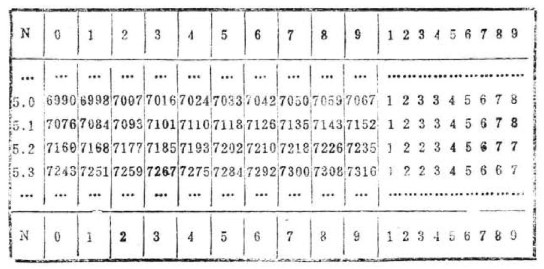
\includegraphics[scale=.8]{fig/1.jpg}
\end{center}


 
下面说明查表求常用对数的方法:
\begin{enumerate}
    \item 当$1\le N<10$时,对数的首数为零,由表中查出的
对数的尾数就是$N$的对数。
\begin{enumerate}[(1)]
 \item 若$N$有三个有效数字,由表就能直接查出$N$的对数。
如查表求$\lg 5.08$, 从$N$所在的直列中找出$5.0$, 从$N$所在的横行中找出8, 那么,5.0所在的行与8所在的列交叉处的数
7059表示的数是0.7059, 就是所求的数,即$\lg5.08=0.7059$。
又如,查表可以求得
$\lg5.3=0.7243$(把5.3看成5.30再查
表),$\lg5=0.6990$(把5看成5.00再查表)。
\item 表中右边顶上一横行是真数的第四个有效数字。若真
数有四个有效数字,就要用到第四个有效数字所对应的修正
值。例如,查表求$\lg5.263$. 真数5.263的第四个有效数字3
对应的修正值2表示0.0002, 因而
$\lg5.263=0.7210+0.0002=0.7212$.
\item 若$N$有五个或更多个有效数字时,可先用四舍五入法
把它改写成四个有效数字,再按(2)中的方法求对数。
\end{enumerate}

\item 当真数$N<1$或
$N\ge 10$时,先用科学记数法把$N$写
成$a\cdot 10^n$的形式,其中
$1\le a<10$, $n\in\Z$。这时$N$的对数的首数
是$n$, 尾数可由$a$从表中查出。
\end{enumerate}

若知道了一个数的常用对数,欲求这个数可查《反对数
表》。如已知$\lg N=0.2846$, 求$N$.

下面是《中学数学用表》中的《反对数表》的一部分。
\begin{center}
    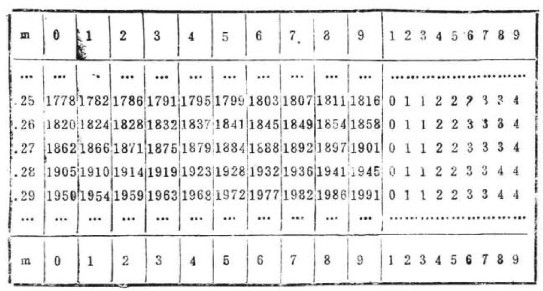
\includegraphics[scale=.8]{fig/2.jpg}
\end{center}

下面说明《反对数表》的查法:
\begin{enumerate}
    \item 当$N$的对数的首数为0时,有$1\le N<10$. 这时从表
中查出尾数对应的四位数字,在第一位数字后面加上小数点,
即得所求的真数$N$. 如已知$\lg N=0.2846$
,求$N$. 在表中$m$所在
的直列中找到.28, 再从$m$所在的横行中找到4, 交叉处的数
是1923, 再查第四位数字6对应的修正值是3, 那么$1923+
3=1926$. 因此,
$N=1.926$
\item 当$N$的对数的首数$n\ne 0$
时,从《反对数表》中查出尾数对应的真数,再将它乘以$10^n$,即得所求的真数。如已知
$\lg N=2.2635$, 求$N$. 由尾数0.2635查表得相应的真数为
1.834, 则
$N=1.834\times 10^2=183.4$.
\end{enumerate}

\begin{ex}
\begin{enumerate}
    \item 已知$\lg x$的尾数与$\lg 7409$的尾数相同,它的首数是下列各
    数,求$x$.
\begin{multicols}{4}
\begin{enumerate}[(1)]
    \item 5
    \item $-2$
    \item 0
    \item $-1$
    \item 1
    \item 3
    \item $-3$
    \item $-4$
\end{enumerate}
\end{multicols}
\item \begin{enumerate}[(1)]
    \item $\lg (100N)$比$\lg\frac{N}{100}$大多少?
    \item $\lg(0.001N)$比$\lg(1000N)$小多少?
\end{enumerate}
\item 已知$\lg 2=0.3010$, $\lg3=0.4771$,求
$\lg0.0015$, $\lg750$.
\item 求下列指数式的值:
\[10^{1.3010},\quad 10^{2.4771},\quad 10^{1.5400},\quad 10^{2.100}\]
\item \begin{enumerate}[(1)]
    \item 确定$2^{100}$
    是几位数,并且求出它的最高的两位数字;
\item $0.3^{100}$    在小数点后面连续有多少个零,并且求出它
    的前两位有效数字。
\end{enumerate}
\end{enumerate}
\end{ex}

\subsection{换底公式}
利用常用对数表,可以求出任意一个正数以10为底的对
数。现在研究如何求出以其他正数
$a\; (0<a\ne 1)$
为底的对数。如求
$\log_3 5=?$

设$\log_{3}5=x$, 转化成指数式$3^{x}=5$。两边再取常用对数,得
$$x\lg3=\lg5\Longrightarrow x=\frac{\lg5}{\lg3}=\frac{0.6990}{0.4771}=1.465,$$
$\therefore \quad \log_3 5= \frac {\lg 5}{\lg 3}= 1.465 $ .

一般地,有下面的\textbf{换底公式}
$$\log_{b}N=\frac{\log_{a}N}{\log_{a}b}\qquad (0<b\neq1,\; 0<a\neq1,\; N>0)$$

\begin{proof}
    设$\log_b N=x$,转化成指数式
$$b^{x}=N$$
两边取以$a$为底的对数,得
$$x\log_{a}b=\log_{a}N $$

$\because \quad b\neq1$,\qquad $\therefore \quad \log_a b\neq 0$.

以$\log_a b$除上式两边,有
\[x=\frac{\log_a N}{\log_a b}\]
即: $\log_b N=\frac{\log_a N}{\log_a b}$
\end{proof}

\begin{note}
\begin{enumerate}
    \item 有了换底公式,就可把以任何实数$a\; (0<a\ne 1)$
    为底
    的对数化为常用对数,从而利用常用对数表即可求出以任何
    实数$a\; (0<a\ne 1)$
    为底的正数$N$的对数;
    \item 在科学技术中常常使用以无理数$e=2.71828\cdots$为底
    的对数,以e为底的对数叫做\textbf{自然对数},$\log_e N$
    通常记作$\ln N$. 
    根据对数换底公式,可以得到自然对数与常用对数之间的关
    系:
    \[\ln N=\frac{\lg N}{\lg e}=\frac{\lg N}{0.4343}\]
    就是
    \[\ln N=2.3031\lg N\]
\item 换底公式是对一些对数式进行恒等变形的重要依据
    之一。
\end{enumerate}
\end{note}

\begin{example}
求证:\begin{enumerate}[(1)]
    \item $\log_a b=\frac{1}{\log_b a}$\quad (或$\log_a b\cdot \log_b a=1$);
此结论可推广为:
\[\log_{a_1}a_2\cdot \log_{a_2}a_3\cdots \log_{a_{n-1}}a_n\cdot \log_{a_n}a_1=1\]
其中:$0<a_k\ne 1$, $k=1,2,\ldots, n$, $n\in\N$,且$n\ge 2$

\item $\log_{a^n}b^n=\log_a b$

其中:$0<a\ne 1$, $b>0$, $n\in\R$

(证明留给读者完成)
\end{enumerate}
\end{example}

\begin{blk}
    分析以下三题应怎样求值:  
\begin{enumerate}[(1)]
    \item $(\log_{4}3+\log_{8}3)(\log_{3}2+\log_{9}2)$
    \item $\log_{8}9\cdot \log_{27}32$
    \item $5^{\log_{25}36}$
\end{enumerate}  
\end{blk}

\begin{example}
\begin{enumerate}[(1)]
    \item 已知$\log_2 9=a$,试以$a$表示$\log_6 16$;
    \item 已知$\log_{12} 27=b$,试以$b$表示$\log_6 16$.
\end{enumerate}
\end{example}

\begin{analyze}
    先将条件式与结论式化简(最好化为同底),然
后再去找联系。
\end{analyze}

\begin{solution}
\begin{enumerate}
    \item \begin{align}
        a&=\log_2 3^2 =2\log_2 3 \tag{1}\\
        \log_{6}16 &= \frac{\log_2 2^4}{\log_2(2\times 3)}=\frac{4}{1+\log_2 3}\tag{2}
    \end{align}
由(1)得:$\log_2 3=\frac{a}{2}$,代入(2),得:
\[\log_6 16=\frac{4}{1+\frac{a}{2}}=\frac{8}{2+a}\]
\item \begin{align}
    b&=\frac{\log_2 3^3}{\log_2(4\times 3)}=\frac{3\log_2 3}{2+\log_2 3}\tag{3}\\
    \log_{6}16&=\frac{\log_2 2^4}{\log_2(2\times 3)}=\frac{4}{1+\log_2 3}\tag{4}
\end{align}
由(3)得:$\log_2 3=\frac{2b}{3-b}$(容易看出$b\ne 3$),代入(4),得:
\[\log_6 16=\frac{4}{1+\frac{2b}{3-b}}=\frac{4(3-b)}{3-b+2b}=\frac{12-4b}{3+b}\]
\end{enumerate}
\end{solution}

\section*{习题三}
\begin{center}
    \bfseries A
\end{center}
\begin{enumerate}
    \item 将下列指数式化为对数式,对数式化为指数式:
\begin{multicols}{2}
\begin{enumerate}[(1)]
    \item $a^0=1$
    \item $a^1=a$
    \item $\log_a\sqrt[3]{a^2}=\frac{2}{3}$
    \item $\log_3\frac{1}{3}\sqrt{3}=-\frac{1}{2}$
\end{enumerate}
\end{multicols}
    \item 计算下列各式:
\begin{multicols}{2}
\begin{enumerate}[(1)]
    \item $5^{1+\log_5 7}$
    \item $2^{8-\log_2 8}$
    \item $8^{\log_2\frac{1}{8}}$
    \item $\sqrt{81^{0.5\times \log_8 11}}$
    \item $27^{\tfrac{2}{3}\log_3 2}$
    \item $40\cdot 100^{\tfrac{1}{2}\lg 9-\lg 2}$
    \item $2^{\log_4\left(2-\sqrt{3}\right)^2}+3^{\log_9\left(2+\sqrt{3}\right)^2}$
\end{enumerate}
\end{multicols}
    \item 若$0<a\ne 1$, $x,y\in\R$,且$xy>0$,下列变形中哪一种是错误
的:
\begin{multicols}{2}
    \begin{enumerate}[(1)]
\item $\log_a x^2=2\log_a x$
\item $\log_a x^2 = 2\log_a |x|$
\item $\log_a (xy)=\log_a x+\log_a y$
\item $\lg_a (xy)=\log_a|x|+ \log_a|y| $
    \end{enumerate}
\end{multicols}
\item 不查表,求值:
    \begin{enumerate}[(1)]
\item $\log_2 (1+\sqrt{2}+\sqrt{3})+\log_2 (1+\sqrt{2}-\sqrt{3})$
\begin{multicols}{2}
\item $\log_{2+\sqrt{3}}(2-\sqrt{3}) $
\item $\log_{\sqrt{2}-1}(3-2\sqrt{2}) $
\item $\log_{\sqrt{3}-\sqrt{2}}(5+2\sqrt{6}) $
\item $\log_{\tfrac{1}{9}}\sqrt[5]{27}$
\end{multicols}
    \end{enumerate}

\item \begin{enumerate}[(1)]
    \item 已知$\lg3=0.4771$, $\lg786=2.8954$,求$\sqrt[5]{0.3}$的值;
\item 利用$\lg72=1.8573$, $\lg108=2.0334$,求$\lg2$与$\lg3$的值。
\end{enumerate}

\item 已知$\lg2=0.3010$, 问$2^7\cdot 8^{11}\cdot 5^{10}$
是几位数?其个位数字是
几?
\item 不查表,求值;
\begin{enumerate}[(1)]
    \item $\lg 98-\lg 2+2\sqrt{\lg^2 7-2\lg 7+1}$
    \begin{multicols}{2}
    \item $\sqrt{5^{2\log_5 (\lg 3)}-2\lg 3+1}$
    \item $\lg^2 2+\lg 4\cdot \lg 50+\lg^2 50$
    \item $\frac{3\lg 2+\lg 3+\lg 5}{1+\frac{1}{2}\lg 36+\frac{1}{3}\lg 8}$
\end{multicols}
\end{enumerate}
\end{enumerate}

\begin{center}
    \bfseries B
\end{center}
    
\begin{enumerate}\setcounter{enumi}{7}
    \item \begin{enumerate}[(1)]
        \item 已知$\ln y=x+\ln C$,求证:$y=Ce^x$
        \item 已知$\ln\frac{y}{x}-ax=\ln C$,求证:$y=Cxe^{ax}$
    \end{enumerate}


\item 设$a^2+b^2=7ab$,且$a>0$, $b>0$,求证:
\[\lg\frac{a+b}{3}=\frac{1}{2}(\lg a+\lg b)\]
\item 设$a^2+b^2=6ab$,且$a>b>0$,求证:
\[\lg\frac{a-b}{3}=\frac{1}{2}(\lg a+\lg b)\]
\item 求证:
\begin{multicols}{2}
 \begin{enumerate}[(1)]
    \item $\frac{\log_5 \sqrt{2}\cdot \log_7 9}{\log_5 \frac{1}{3}\cdot \log_7 \sqrt[3]{4}}=-\frac{3}{2}$
    \item $\log_4 8-\log_{\tfrac{1}{9}}3-\log_{\sqrt{2}}4=-2$
\end{enumerate}   
\end{multicols}

\item 已知$\log_2 3=m$, $\log_3 7=n$
试用$m,n$表达$\log_{42}56$的值。
\item 已知$\log_{18}9=a$, $18^b=5$,
试用$a$、$b$表示$\log_{36}45$的值。
\item 设正数$A$、$B$、$C$的常用对数分别是$a$、$b$、$c$, 且
$a+b+c=0$,求证
\[A^{\tfrac{1}{b}+\tfrac{1}{a}}\cdot B^{\tfrac{1}{c}+\tfrac{1}{a}}\cdot C^{\tfrac{1}{a}+\tfrac{1}{b}}=\frac{1}{1000}\]
\item 若$y=a^{\tfrac{1}{1-\log_a x}}$, $z=a^{\tfrac{1}{1-\log_a y}}$, 则$x=a^{\tfrac{1}{1-\log_a z}}$

\item 若$a$、$b$、$c$为${\rm Rt}\triangle$的三边长,其中$c$为斜边长。
则
\[\log_{b+c}a+\log_{c-b}a=2\log_{b+c} a\cdot \log_{c-b} a\]
\end{enumerate}


\section{对数函数及其图象和性质}

\subsection{对数函数}
指数函数$y=a^x\; (0<a\ne 1)$的反函数叫做对数函数,记作$y=\log_a x\; (0<a\ne 1)$.

对数函数$y=\log_a x$的定义域就是指数函数
$y=a^x$的值域$(0,+\infty)$;对数函数
$y=\log_a x$的值域就是指数函数
$y=a^x$的定义域$\R$.

\begin{figure}[htp]
    \centering
\begin{tikzpicture}[>=stealth]
\draw[->](-2,0)--(5,0)node[right]{$x$};
\draw[->](0,-2)--(0,5)node[right]{$y$};
\draw[dashdotted](-1.5,-1.5)--(4,4)node[above]{$y=x$};
\node [below right]{$O$};
\foreach \x in {-1,1,2,3,4}
{
    \draw(\x,0)node[below]{$\x$}--(\x,.1);
    \draw(0,\x)node[left]{$\x$}--(.1,\x);
}

\draw[domain=-1.5:.65, smooth, thick]plot(\x, 10^\x)node[above right]{$y=10^x$};
\draw[domain=-1.5:.65, smooth, thick]plot(10^\x,\x)node[above]{$y=\log_{10}x$};

\draw[domain=-1.75:2, smooth, very thick]plot(\x, 2^\x)node[above right]{$y=2^x$};
\draw[domain=-1.75:2, smooth, very thick]plot(2^\x,\x)node[above]{$y=\log_{2}x$};

\draw[domain=1.5:-1.75, smooth, ultra thick]plot(\x, 0.5^\x)node[above]{$y=\left(\frac{1}{2}\right)^x$};
\draw[domain=1.5:-1.75, smooth, ultra thick]plot(0.5^\x,\x)node[right]{$y=\log_{\tfrac{1}{2}}x$};

\end{tikzpicture}
    \caption{}
\end{figure}



\subsection{对数函数的图象和性质}
由于指数函数与对数函数互为反函数,因此指数函数
$y=a^x\; (0<a\ne 1)$与对数函数
$y=\log_a x\; (0<a\ne 1)$的图象
关于直线$y=x$对称(图3.15).

对数函数在其底$a>1$
及$0<a<1$这两种情况下的图象和
性质,见表3.3:

\begin{table}[htp]
    \centering
    \caption{}
    \begin{tabular}{c|cc}
\hline
& $a>1$&$0<a<1$\\
\hline
底数$a$对图象的影响& \multicolumn{2}{c}{$y=\log_a x $与$y\log_{\tfrac{1}{a}}x$的图象关于$x$轴对称}\\
定义域& $\R^+$&$\R^+$\\
值域& $\R$&$\R$\\
& \multicolumn{2}{c}{任意实数$k$都能写成对数形式$k=\log_a a^k$}\\
单调性& 增函数&  减函数\\
&$\log_a x=\begin{cases}
    >0, & x>1\\=0,& x=1\\ <0& x<1
\end{cases}$ & $\log_a x=\begin{cases}
    <0, & x>1\\=0,& x=1\\ >0& x<1
\end{cases}$ \\
关键点& $(1,0)$, $(a,1)$ &$(1,0)$, $(a,1)$\\
\hline
    \end{tabular}
\end{table}

这里,类似于指数函数也应做几点说明(请读者自己考
虑)。

\begin{center}
\begin{tikzpicture}[>=stealth]
\begin{scope}
    \draw[->](-1,0)--(3,0)node[right]{$x$};
    \draw[->](0,-1)--(0,3)node[right]{$y$};
\node [below left]{$O$};
\foreach \x in {1,2}
{
    \draw(\x,0)node[below]{$\x$}--(\x,.1);
    \draw(0,\x)node[left]{$\x$}--(.1,\x);
}
\node at (1,-2){$(a>1)$};
\draw[domain=-1:1.5, smooth, very thick]plot(2^\x, \x)node[above]{$y=\log_a x$};

\end{scope}
\begin{scope}[xshift=5cm]
\draw[->](-1,0)--(3,0)node[right]{$x$};
\draw[->](0,-1)--(0,3)node[right]{$y$};
\node [below left]{$O$};
\foreach \x in {1,2}
{
    \draw(\x,0)node[below]{$\x$}--(\x,.1);
    \draw(0,\x)node[left]{$\x$}--(.1,\x);
}
\node at (1,-2){$(0<a<1)$};
\draw[domain=1.5:-1, smooth, very thick]plot(0.4^\x, \x)node[below left]{$y=\log_a x$};

\end{scope}
\end{tikzpicture}
\end{center}

这里,类似于指数函数也应做几点说明(请读者自己考虑)。

\begin{example}
    在同一坐标系中,画出函数$y=\log_2 x$, $y=\log_3 x$, $y=\log_{\tfrac{1}{2}}x$, $y=\log_{\tfrac{1}{3}}x$的图象。
\end{example}

\begin{solution}
    利用描点法先画出$y=\log_2 x$与$y=\log_3 x$
的图象,再
利用关于$x$轴的对称性画出$y=\log_{\tfrac{1}{2}}x$与$y=\log_{\tfrac{1}{3}}x$
的图象。
\end{solution}

\begin{note}
    从图3.16可以看出,当底数
$a>1$时,$a$越大曲线越靠
近$x$轴与$y$轴,这同指数函数的情况是一致的(为什么?),
而当$0<a<1$时,结论恰恰相反。
\end{note}

\begin{figure}[htp]
    \centering
\begin{tikzpicture}[>=stealth]
\draw[->](-1,0)--(6,0)node[right]{$x$};
\draw[->](0,-3)--(0,3)node[left]{$y$};
\node [below left]{$O$};
\foreach \x in {1,2,3,4,5}
{
    \draw(\x,0)node[below]{$\x$}--(\x,.1);
}
\foreach \x in {-1,-2,1,2}
{
    \draw(0,\x)node[left]{$\x$}--(.1,\x);
}

\draw[domain=-1.5:1.6, smooth, thick]plot(3^\x,\x)node[below]{$y=\log_{3}x$};

\draw[domain=-1.75:2.4, smooth, very thick]plot(2^\x,\x)node[above]{$y=\log_{2}x$};

\draw[domain=-1.5:1.6, smooth, dashed, thick]plot(3^\x,-\x)node[above]{$y=\log_{\tfrac{1}{3}}x$};

\draw[domain=-1.75:2.4, smooth,  dashed,very thick]plot(2^\x,-\x)node[below]{$y=\log_{\tfrac{1}{2}}x$};

\foreach \x in {(2,1), (4,2)}
{
    \fill \x circle(2pt)node[above]{$\x$};
} 

\fill (3,1) circle(2pt)node[below]{$(3,1)$};
\foreach \x in {(2,-1), (4,-2)}
{
    \fill \x circle(2pt)node[above]{$\x$};
}
\fill (3,-1)circle(2pt)node[above right]{$(3,-1)$};
\fill(.5,1) circle(2pt)node[above right]{$\left(\tfrac{1}{2},1\right)$};
\fill(.5,-1) circle(2pt)node[below right]{$\left(\tfrac{1}{2},-1\right)$};


\end{tikzpicture}
    \caption{}
\end{figure}


\begin{example}
\begin{enumerate}[(1)]
    \item 若$\log_a 3>\log_b 3>0$,则$a$、$b$、1的大小顺序是\blank;
    \item 若$\log_a 0.3<\log_b 0.3<0$,则$a$、$b$、1的大小顺序是\blank。
\end{enumerate}
\end{example}

\begin{analyze}
    从图3.15可以直观地看出结论,也可以通过对条件式的变形解决问题。
\end{analyze}

\begin{solution}
\begin{enumerate}[(1)]
    \item 从图3.15可见,当$x\in (1,+\infty)$时,对于相同的$x$,若$y>0$(即$a>1$)时,必有$a$越大,$y$越小,从而知道$1<a<b$.
    
    若从$\log_a 3>\log_b 3>0$变形着手,有
\[\frac{1}{\log_3 a}>\frac{1}{\log_3 b}>0 \qquad \text{(化异底为同底)}\]

$\therefore\quad \log_3 b>\log_3 a>0\Longrightarrow \log_3 b>\log_3 a>\log_3 1$

利用$\log_3 x$是增函数,立刻有$b>a>1$.
\item 当$\log_a 0.3<\log_b 0.3<0$时,有
\[\frac{1}{\log_{0.3} a}<\frac{1}{\log_{0.3} b}<0\]

$\therefore\quad 0>\log_{0.3} a>\log_{0.3} b \Longrightarrow \log_{0.3} 1>\log_{0.3} a>\log_{0.3} b$

利用$\log_{0.3} x$是减函数,立刻有$1<a<b$.
\end{enumerate}
\end{solution}

\begin{example}
求下列函数的定义域:
\begin{multicols}{2}
\begin{enumerate}[(1)]
    \item $y=\log_{0.1}|x|$
    \item $y=\log_3 (4-x^2)$
    \item $y=\frac{1}{\log_3(3x+5)}$
    \item $y=\sqrt{\log_{0.1}(4x-3)}$
\end{enumerate}
\end{multicols}
\end{example}

\begin{solution}
\begin{enumerate}[(1)]
    \item $D=\{x\mid x\in\R,\; x\ne 0\}$
    \item $4-x^2>0,\; x\in(-2,2)$
    
$\therefore\quad D=(-2,2)$

\item 要使$y$有意义,须$\log_3(3x+5)\ne 0$,即$\begin{cases}
    3x+5\ne 1\\ 3x+5>0
\end{cases}$

$\therefore\quad 0<3x+5\ne 1\Longleftrightarrow -\frac{5}{3}<x\ne -\frac{4}{3}$

$\therefore\quad D=\left(-\frac{5}{3},-\frac{4}{3}\right)\cup\left(-\frac{4}{3},+\infty\right)$

\item 要使$y$有意义,须$\log_{0.1}(4x-3)\ge 0$,即$0<4x-3\le 1$,

解之,得
$\frac{3}{4}<x\le 1$

$\therefore\quad D=\left(\frac{3}{4}, 1\right]$
\end{enumerate}
\end{solution}

\begin{example}
    比较下列各题中两个数的大小。
    \begin{multicols}{2}
\begin{enumerate}[(1)]
    \item $\log_3 2.1$与$\log _3 2.8$
    \item $\log_{0.2}7.1$与$\log_{0.2}5.4$
    \item $\log_{a}4.4$与$\log_a 5.5$\quad $(0<a\neq1)$
    \item $(\lg a)^{8.1}$与$(\lg a)^{2.5}$\quad $(1<a\neq10)$
\end{enumerate}        
    \end{multicols}

\end{example}

\begin{solution}
\begin{enumerate}[(1)]
\item $\because \quad $对数函数$y=\log_3 x$单调递增,且$2.1<
2.8$, 

$\therefore\quad \log_3 2.1<\log_3 2.8$
\item $\because\quad $对数函数 $y=\log_{0.2}x$ 单调 递减,且$7.1>
5.4$

$\therefore\quad \log_{0.2}7.1<\log_{0.2}5.4$
\item 当$a>1$时,$y=\log_3 x$单调递增,且$4.4<5.5$,

$\therefore\quad \log_a 4.4< \log _{a}5.5$

当$0<a<1$时, $y=\log_a x$单调递减,且$4.4<5.5$,

$\therefore \quad \log_a 4.4> \log_a 5.5$
\item 当$a\in(1,10)$时,$0<\lg a<1$, 指数函数
$y=(\lg a)^{x}$单调递减,且$3.1>2.5$,

$\therefore\quad (\lg a)^{8.1}<(\lg a)^{2.5}$

当$a\in(10,+\infty)$时,$\lg a>1$, 指数函数
$y=(\lg a)^{x}$单调递增,且$3.1>2.5$,

$\therefore\quad (\lg a)^{8.1}>(\lg a)^{2.5}$
\end{enumerate}
\end{solution}

\begin{example}
 比较$\log_3 0.4$ 与$-\frac12$的大小.   
\end{example}

\begin{analyze}
    不同类的对象难以比较。根据“任一实数都能写
成对数形式”,先把$-\frac12$写成对数.
\end{analyze}

\begin{solution}
    \[- \frac 12= \log_3 3^{- \frac 12}= \log_{3}\frac {\sqrt {3}}3\]

$\because \quad y= \log_3 x$ 单调递增,且$0.4<\frac{\sqrt{3}}{3}.$

$\therefore \quad \log_3 0.4< \log_{3}\frac{\sqrt{3}}{3}$, 即$\log_3 0.4< - \frac 12.$    
\end{solution}

\begin{example}
    比较下列各题中两个数的大小
\begin{multicols}{2}
\begin{enumerate}[(1)]
    \item $\log_2 3$与$\log_7 6$
    \item $\log_{0.2}0.4$与$\log_2 0.7$
\end{enumerate}
\end{multicols}
\end{example}

\begin{analyze}
  因为两对数的底不同,故不能直接利用对数函数
的单调性比大小。若用换底公式做,也难以奏效。我们用
“中间值法”试一试。 常用的中间值是0或1.  
\end{analyze}

\begin{solution}
\begin{enumerate}[(1)]
    \item $\because\quad \log_2 3 >1$ ($\because\quad \log_2 3>\log_2 2=1$)
    
而$\log_7 6<1$ ($\because\quad \log_7 6<\log_7 7=1$)

$\therefore\quad \log_2 3 >\log_7 6$
\item $\because\quad \log_{0.2} 0.4 >0$ ($\because\quad \log_{0.2} 0.4>\log_{0.2} 1=0$)
    
而$\log_2 0.7<0$ ($\because\quad \log_2 0.7<\log_2 1=0$)

$\therefore\quad \log_{0.2} 0.4 >\log_2 0.7$
\end{enumerate}
\end{solution}

\begin{example}
    解不等式:
\begin{multicols}{2}
   \begin{enumerate}[(1)]
\item $\log_{0.1}(x^2-2x-2)>0$;
\item $\log_a(x^2-x)\ge \log_a (x+1)\quad (a>1)$
\end{enumerate} 
\end{multicols}

\end{example}

\begin{analyze}
    解不等式就是求未知数$x$的取值范围。就对数不等式而言,当然既要考虑对数函数的定义域,又要考虑对数函数的增减性。
\end{analyze}

\begin{solution}
\begin{enumerate}[(1)]
    \item 由于$\log_{0.1}1=0$,原不等式可改写成
\begin{equation}
    \log_{0.1}(x^2-2x-2)>\log_{0.1}1   \tag{1}
\end{equation}
由(1)
\begin{align}
    x^2-2x-2>0, \quad \text{(由定义域)} \tag{2}\\
    x^2-2x-2>0, \quad \text{(由增减性)} \tag{3}
\end{align}
解(2), 得 $x<1-\sqrt{3}$, 或$x>1+\sqrt{3}$

解(3), 得 $-1<x<3$

$\therefore\quad $原不等式的解集为$(-1,1-\sqrt{3})\cup (1+\sqrt{3},3)$.

\item 根据原不等式
\begin{align}
    x^2-x>0,&\quad \text{(由定义域)} \tag{4}\\
    x+1>0,&\tag{5}\\
    x^2-x\ge x+1,&\quad \text{(由增减性)} \tag{6}
\end{align}

由(5)、(6)可推得(4),所以(4)可省掉。

解(5),得$x>-1$;解(6),得$x\le 1-\sqrt{2}$,或$x\ge 1+\sqrt{2}$.

$\therefore\quad $原不等式的解集为
\[\left(-1,1-\sqrt{2}\right]\cup \left[1+\sqrt{2},+\infty\right)\]
\end{enumerate}
\end{solution}

\begin{note}
    解对数不等式的基本方法是转化为代数不等式组,这种转化既要考虑定义域,又要考虑增减性,否则前后可能不同解(不等价)。

    当式子中含参数时,要树立“讨论”的意识,如例4中的(3)、(4)。
\end{note}

\begin{example}
求证:$2<\frac{1}{\log_2 19}+\frac{2}{\log_3 19}+\frac{2}{\log_5 19}<3$
\end{example}

\begin{analyze}
    将三个不同底的对数化成同底。
\end{analyze}

\begin{proof}
\[\begin{split}
    \frac{1}{\log_2 19}+\frac{2}{\log_3 19}+\frac{2}{\log_5 19}&=\log_{19}2+2\log_{19}3+2\log_{19}5\\
    &=\log_{19}(2\times 3^2\times 5^2)=\log_{19}450
\end{split} \]
利用$\log_{19}x$是增函数,得
\[2=\log_{19}19^2<\log_{19}450<\log_{19}19^3=3\]

$\therefore\quad 2<\frac{1}{\log_2 19}+\frac{2}{\log_3 19}+\frac{2}{\log_5 19}<3$
\end{proof}

\begin{example}
求函数$y=\log_a(x^2-2x)$的单调区间。
\end{example}

\begin{analyze}
这个函数可看作是由$y=\log_a u\; (0<a\ne 1)$与$u=x^2-2x$复合而成的。由于$0<a<1$和$a>1$时$\log_a u$的增减性不同,因此应分情况进行讨论;另一方面又要考虑到函数$y=\log_a(x^2-2x)$的定义域为$(-\infty,0)\cup (2,+\infty)$.
\end{analyze}

\begin{solution}
\begin{enumerate}[(1)]
    \item 若$0<a<1$时,$\log_{a}u$为单调减函数,而函数$u=x^2-2x=(x-1)^2-1$在$(-\infty,1)$上单调减,在$(1,+\infty)$上单调增。故$(-\infty,0)$是函数$y=\log_{a}(x^{2}-2x)$的单调增区间,$(2,+\infty)$是函数的单调减区间。
    \item 若$a>1$时,则$(-\infty,0)$ 是函数$y=\log_a(x^2-2x)$的单调减区间,$(2,+\infty)$是函数的单调增区间。
\end{enumerate}
\end{solution}

\section*{习题四}
\begin{center}
    \bfseries A
\end{center}

\begin{enumerate}
    \item 证明:在同一坐标系中函数$y=\log_a x$与$y=\log_{\tfrac1a}x\; (0<a\neq1)$的图象关于$x$轴对称。
    \item 求下列函数的定义域:
\begin{multicols}{2}
\begin{enumerate}[(1)]
    \item $y=\log_5(1+x)$
    \item $y=\frac{1}{\ln x}$
    \item $y=\log_{0.1}\frac{1}{1-3x^2}$
    \item $y=\sqrt{\log_3 x}$
    \item $y=3\sqrt{\log_2 x}$
    \item $y=\sqrt{\log_{0.2}(3-2x)}$
    \item $y=\sqrt{\lg(2x^2-9x-4)}$
    \item $y=\frac{\sqrt{1-\frac{2}{3}|x|}}{\log_{0.1}(x+1)}$
\end{enumerate}
\end{multicols}

\item 若$\log_5 6\cdot \log_6 7\cdot \log_7 8\cdot \log_8 9\cdot \log_9 10=m$,那么$m$的值属于下列哪个区间:
\[(0,1),\qquad (1,2),\qquad (2,3),\qquad (3,4)\]
\item 比较下列各题中两个数的大小:
\begin{multicols}{2}
\begin{enumerate}[(1)]
    \item $\log_5 7.8$与$\log_5 9.2$
    \item $\log_{0.3}5$与$\log_{0.3}8$
    \item $\lg 0.75$与$\lg 0.85$
    \item $\ln108$与$\ln105$
    \item $\log_{0.2}0.7$与$\log_5 0.8$
    \item $\ln 4.9$与$\log_{\tfrac{1}{\sqrt{2}}}8.5$
    \item $\log_{\tfrac{3}{2}}\frac{3}{4}$与$\log_{\tfrac{1}{3}}\frac{2}{3}$
    \item $\log_a 3.14$与$\log_a \pi\; (0<a\ne 1)$
    \item $(\lg m)^{-3.1}$与$(\lg m)^{-2.4}$ 
    
    $(m>1)$
    \item $\log_{10}a$与$\log_a 10\quad (a>1)$
    \item $\log_a b$与$\log_{\tfrac{1}{a}}b\quad (0<a<1)$
\end{enumerate}
\end{multicols}
\item 填空:
\begin{enumerate}[(1)]
    \item $\log_{\tfrac{1}{2}}x<2$的解集是\blank.
    \item $\log_{\sqrt{2}}x<6$的解集是\blank.
    
    (提示:把右边的常数写成对数形式)
    \item 设$f(x)=\log_2 x$,则$[f(x)]^2>f(x^2)$的解集是\blank.
\end{enumerate}

\item 解下列不等式:
\begin{enumerate}[(1)]
    \item $\log_{0.2}(x^2+x-1)\ge 0$
    \item $\lg (x^2+21x)>2$
    \item $\log_{0.2}(x^2-3x-4)\ge \log_{0.2}(2x+10)$
\end{enumerate}
\end{enumerate}

\begin{center}
    \bfseries B
\end{center}

\begin{enumerate}\setcounter{enumi}{6}
    \item 设$\frac{1}{\log_{\tfrac{1}{2}}\frac{1}{3}}+\frac{1}{\log_{\tfrac{1}{5}}\frac{1}{3}}=n$,那么$n$属于下列哪个区间:
    \[(-2,-1),\quad (1,2),\quad (-3,-2),\quad (2,3)\]
\item 求证:
\begin{enumerate}[(1)]
\item $2< \frac 1{\log _{13}7}+ \frac 1{\log _{5}7}< 3$ ,

\item $4< \frac 3{\log _{2}e}+ \frac 2{\log _{3}e}< 5$ ,

\item $1< \frac 1{\log _{2}11}$ $+ \frac 1{\log _{3}11}$ $+ \frac 1{\log _{4}11}$ $+ \frac 1{\log _{5}11}< 2$.
\end{enumerate}
\item  若$\log_m(e-2)>\log_n(e-2)>0$, 试指出$m,n$与1的大
小顺序。
\item 解不等式:
$\log_{a}\left(2x^{2}-4x\right)\ge \log_{a}\left(x^{2}-4x+1\right)、\quad (0<a\neq1).$
\item 解下列不等式:
\begin{enumerate}[(1)]
    \item $\frac 1{\log _2x}- \frac 1{\log _2x- 1}< 1$
    \item $\log_{x}5- 2\log_{\sqrt {5}}x> 3\quad ( x> 1) $
    \item $\log_2\left(\frac23\right)^x+\log_2\left(\frac49\right)^{2x}<\log_2\left(\frac23\right)^5$
    \item $\log_2 x-\log_{\sqrt{x}}2<1 $
    \item $\log_{kx}x+\log_x (kx)^2>0\quad (0<k<1)$
    \item $\frac{1}{\log_{x-1}4}-\frac{1}{\log_{5-x}4}>0$
    \item $\log_{\tfrac{1}{2}}\left|\frac{1}{x-1}\right|>\log_{\tfrac{1}{2}}\left|\frac{2}{x+3}\right|+1$
\end{enumerate}

\item 求下列函数的单调减区间:
\begin{multicols}{2}
\begin{enumerate}[(1)]
    \item $y=\log_a (-x^2+6x-5)$
    \item $y=2^{|\lg x|}$
\end{enumerate}
\end{multicols}
\item 判断函数$f(x)=\lg\left(x+\sqrt{x^2+1}\right)$的奇偶性。
\end{enumerate}

\section{指数方程和对数方程}
在指数中含有未知数的方程叫做\textbf{指数方程}。

在对数记号中的真数或底数中含有未知数的方程叫做\textbf{对数方程}。

在这两类方程中,我们只能解一些特殊的方程。请看下面的例子。

\begin{example}
    解方程$4^x=2^{x+1}$.
\end{example}

\begin{solution}
    原方程可化为$$2^{2x}=2^{x+1}$$
根据指数函数
$y=2^u\; (u\in\R)$
的单调性,两个同底的幂相等,
当且仅当它们的幂指数相等,所以上面的方程同解于(或说
成“等价于”,记为$\Longleftrightarrow$)
\[2x=x+1\] 
$\therefore\quad x=1$.
\end{solution}

\begin{note}
    这里决定性的一步是把两个幂“化成同底”。
\end{note}

\begin{example}
     解方程$3^{x+1}+9^x-18=0$.
\end{example}

\begin{solution}
    原方程可化为
\[3\cdot 3^x +(3^x)^2-18=0\]
令$3^x=y$,这个方程就写成
\[y^2+3y-18=0\]
解之得:$y_1=3,\qquad y_2=-6$

由$3^x=3$,得$x=1$;
$3^x=-6$
不符合指数函数的性质,应
舍去。

$\therefore\quad $原方程的解是
$x=1$.
\end{solution}

\begin{note}
    这里使用换元法:
$y=3^x$,是解方程或不等式常
用的方法之一。
\end{note}

\begin{blk}
    方程
$2^{x+1}+3\cdot 2^{1-x}-8=0$
能用换元法解吗?
\end{blk}

\begin{example}
   某厂生产的彩电的台数,如果每年平均比上一年
增长10.4\%,约过多少年产量才能翻一番(结果保留一个有
效数字)? 
\end{example}

\begin{solution}
    设约过$x$年,产量可以翻一番,由题意可得
\[1\cdot (1+10.4\%)^x=2\]
即:$1.104^x=2$,两边取对数,得:
\[x\lg 1.104=\lg 2\]

$\therefore\quad x=\frac{\lg 2}{\lg 1.104}=\frac{0.3010}{0.0429}\approx 7$

答:约经过7年.
\end{solution}

以上三例讲的是\textbf{解指数方程的基本方法}:同底法(关键
是能化成
$a^{f(x)}=a^{g(x)}$
的形式,其中
$0<a\ne 1$);换元法(关
键是能看得出隐含了哪个“元”);取对数法。

\begin{example}
  解方程
  \begin{equation}
 \lg(x^2+11x+8)-\lg(x+1)=1\tag{1}     
  \end{equation}
\end{example}

\begin{solution}
    方程(1)等价于(同解于)
\[\begin{cases}
    x^2+11x+8>0,&\text{(由定义域)}\\
    x+1>0,&\text{(由定义域)}\\
    \lg\frac{x^2+11x+8}{x+1}=\lg10,&\text{(由单调性)}\\
\end{cases}\Longleftrightarrow \begin{cases}
    x^2+11x+8>0,&(2)\\
    x+1>0,&(3)\\
    \frac{x^2+11x+8}{x+1}=10,&(4)
\end{cases}\]
解(4),得:$x_1=-2,\quad x_2=1$

$x_1$不满足(3), 舍去;$x_2$满足(2)、(3)

$\therefore\quad x=1$是(1)的解.
\end{solution}

\begin{note}
    解对数方程时,首先应考虑定义域,从而转化为
代数不等式与方程的混合组。\textbf{解混合组的一般方法}是先求出
方程的解,再把它代入不等式。若都适合,它就是混合组的
解,否则,一定不是混合组的解。
\end{note}

\begin{example}
    解方程
    \begin{equation}
\log_2(5x^2-1)-1=\log_2 x+log_2 2x \tag{1}
    \end{equation}
\end{example}

\begin{solution}
\[\text{方程(1)}\Longleftrightarrow\begin{cases}
    x>0, \quad \text{(由定义域)}& (2)\\
    \log_2\frac{5x^2-1}{2}=\log_2(x\cdot 2x), &(3)
\end{cases}\]
\[(3)\Longleftrightarrow \begin{cases}
    5x^2-1>0\\
    x\ne 0\\
    \frac{5x^2-1}{2}=2x^2
\end{cases}\]
解之,得:$x_1=1,\quad x_2=-1$.

$x_1=1$适合(2);$x_2=-1$不适合(2),舍去。

$\therefore\quad x=1$是(1)的解。
\end{solution}


\begin{example}
    解方程
    \begin{equation}
        2log_{25}x+\log_x 25=3 \tag{1}
    \end{equation}
\end{example}

\begin{solution}
\begin{equation}
    (1)\Longleftrightarrow 2\log_{25}x+\frac{1}{\log_{25}x}=3 \tag{2}
\end{equation}
令$\log_{25}x=y$,则(2)变为
\[2y+\frac{1}{y}=3\Longleftrightarrow 2y^2-3y+1=0\; (y\ne 0)\]
解之,得:$y_1=1,\quad y_2=\frac{1}{2}$.

由$\log_{25}x=1$,得$x_1=25$;
由$\log_{25}x=\frac{1}{2}$,得$x_2=25^{\tfrac{1}{2}}=5$. $x_1,x_2$都适合(2)

$\therefore\quad $方程(1)的解集是$\{25,5\}$
\end{solution}


\begin{example}
    解方程
\begin{equation}
    \log_{2x^2-1}(3x^{2}-2x-1)=1 \tag{1}
\end{equation}
\end{example}

\begin{solution}
\[\text{方程(1)}\Longleftrightarrow \begin{cases}
    3x^{2}-2x-1>0,\quad \text{(由定义域)}& (2)\\
    0<2x^2-1\ne 1 & (3)\\
    3x^{2}-2x-1=2x^2-1 ,\quad \text{(由单调性)}& (4)
\end{cases}\]
解(4), 得 $x_1=0,\quad x_2=2$。

$x_1$不满足(2), 是增根,舍;$x_2$满足(2)、(3).

$\therefore \quad x= 2$是原方程的解。
\end{solution}

以上四例讲的是\textbf{解对数方程的基本方法}:转化成同解的
混合组,或者用换元法处理。

再研究几个例题。

\begin{example}
    解方程$x^{2\lg x}=10\cdot  x$
\end{example}

\begin{analyze}
    在幂$x^{2\lg x}$的底数与指数中都含有$x$, 但等号两边同取以10为底的对数(应该想到,两边都为正数,所以允许取对数),原方程就变成以$\lg x$为元的方程了。
\end{analyze}

\begin{solution}
    由于$x>0$, 方程两边皆正,取常用对数,得
$$2\lg x\cdot \lg x=1+lg x$$
令$\lg x= y$, 得$2y^2- y- 1= 0$。解之,得$y_1=1,\quad y_2=-\frac{1}{2}$.

由$\lg x=1$,得$x=10$;由$\lg x=-\frac{1}{2}$,得$x=\frac{\sqrt{10}}{10}$.

经检验,$x_1=10$,$x_2=\frac{\sqrt{10}}{10}$都是原方程的解。
\end{solution}

\begin{example}
    解不等式$x^{\log_a x}>\frac{x^{\tfrac{9}{2}}}{a^2}$
\end{example}

\begin{analyze}
    取以$a$为底的对数,就变成以$\log_a x$为元的不等式了。
\end{analyze}

\begin{solution}
由于$x>0$,不等式两边皆正,可以取以$a$为底的对数。
\begin{enumerate}
    \item 当$a>1$时,$\log_a u$是$u$的增函数,得:
    \[\log_a x\cdot \log_a x>\frac{9}{2}\log_a x-2\log_a a\]
令$\log_a x=y$,得:$2y^2-9y+4>0$,解之,得:$y<\frac{1}{2}$或$y>4$,即:
\[\log_a x<\frac{1}{2},\quad \text{或}\quad \log_a x>4\]

$\therefore\quad 0<x<\sqrt{a}$,或$x>a^4$.

\item 当$0<a<1$时,$\log_a u$是$u$的减函数,得
\[\log_a x\cdot \log_a x< \frac{9}{2}\log_a x-2\log_a a\]
令$\log_a x=y$,得:$2y^2-9y+4<0$,解之,得:$\frac{1}{2}<y<4$,即:
\[\frac{1}{2}<\log_a x<4\Longleftrightarrow \log_a a^{\tfrac{1}{2}}<\log_a x<\log_a a^4\]

$\therefore\quad \sqrt{a}>x>a^4$
\end{enumerate}
\end{solution}

\begin{note}
    解题中,当需要对不等式两边取以$a$为底的对数
时,要特别注意参数$a$的不同取值对对数函数增减性的影响,
通过此例应很好地理解这一点。
\end{note}



\begin{example}
解方程:
\begin{multicols}{2}
\begin{enumerate}[(1)]
    \item $x+\lg x=3$
    \item $2^x=\log_3(x+3)$
\end{enumerate}
\end{multicols}
\end{example}

\begin{analyze}
    这两个方程都是我们未曾见过的类型。无现成模
式可用。此时,“转化”的思想有可能使我们找到解决问题的
途径。

对于(1)原方程改写作
\begin{equation}
    \lg x=3-x\tag{1}
\end{equation}
令$f(x)=\lg x$,$g(x)=3-x$
。以函数的观点来看,方程(1)的解
就是使$f(x)$与$g(x)$
的函数值相等的$x$值。而这两个函数都是
我们所熟知的,从而,可用图象法解决问题。
\end{analyze}

\begin{figure}[htp]
    \centering
\begin{minipage}{.45\textwidth}
    \begin{tikzpicture}[>=stealth, scale=.7]
\draw[->](-1,0)--(5,0)node[right]{$x$};
\draw[->](0,-2)--(0,5)node[left]{$y$};
\node[below left]{$O$};
\draw[domain=-1:4.5, very thick]plot(\x, 3-\x)node[left]{$y=3-x$};
\draw[domain=.1:4.5, very thick, smooth]plot(\x,{log10(\x)})node[above]{$y=\lg x$};
\foreach \x in {1,2,3,4}
{
    \draw(\x,0)node[below]{\x}--(\x,.1);
}        
\node at (2.6,.5)[above]{$A$};
\end{tikzpicture}
 \caption{}    
\end{minipage}\hfill
   \begin{minipage}{.45\textwidth}
    \begin{tikzpicture}[>=stealth, scale=.7]
    \draw[->](-4,0)--(3,0)node[right]{$x$};
\draw[->](0,-3)--(0,4)node[left]{$y$};
\node[below left]{$O$};        

\draw[domain=-3:1.5, very thick]plot(\x, 2^\x)node[above]{$y=2^x$};
\draw[domain=-2.8:2.5, very thick, smooth]plot(\x,{log2(\x+3)/log2(3)})node[below]{$y=\log_3(x+3)$};
\foreach \x in {1,-2,-3,-1,2}
{
    \draw(\x,0)node[below]{\x}--(\x,.1);
}    
\foreach \x in {1,2}
{
    \draw(0,\x)node[left]{\x}--(.1,\x);
}   
\node at (0,1)[below right]{$B$};
\node at (-1.8,.4)[above]{$A$};
\end{tikzpicture}
 \caption{}    
\end{minipage}
\end{figure}




\begin{solution}
\begin{enumerate}[(1)]
    \item 在同一坐标系中分别作出$f(x) = \lg x$与$g(x)=3-x$的图象(图3.17). 两图象相交于$A$ 点(此时,两个函数值相等),$A$的横坐标$x\approx2.6$. 这个值近 似地使$f(x)=g(x)$. 所以,$x=2.6$ 是方程(1)的近 似解,也就是原方程的近似解。(应该看 到,对于(1)我们是无法 求出它的准确解的,想想这是为什么?)
    \item 类似于(1), 用图象法。在同一坐标系中分别作出函数$f(x)=2^{x}$与$g(x)=\log_{3}(x+3)$的图象(图3.18)。两图象相交于$A,B$两点。从图上可以看出点$A$的横坐标$x_1\approx-1.8$, 点$B$的横坐标$x_2=0$. 所以$x_1=-1.8$是方程(2)的近似解,$x_2=0$是(2)的解。
\end{enumerate}
\end{solution}

\begin{note}
此例使我们又一次看到:方程、不等式、函数之
间的密切关系。一般说来,运用函数的观点去透视方程和不
等式的问题常常有助于问题的解决。
\end{note}    

\begin{example}
方程$\lg(ax)\lg(ax^2)=4$的所有的解都大于1,求实数$a$的范围。
\end{example}

\begin{solution}
$\because\quad ax^2>0,\; ax>0$, \qquad $\therefore\quad a>0,\; x>0$.

原方程可写成
\begin{equation}
   2\lg^2 x+3\lg a\cdot \lg x+\lg^2 a-4=0 \tag{1} 
\end{equation}

$\because\quad $方程所有的解都大于1,

$\therefore\quad $以$\lg x$为元的方程(1)的所有的解都大于0。于是:
\[\begin{cases}
\Delta =(3\lg a)^2-4\cdot 2(\lg^2 a-4)\ge 0\\
\frac{-3\lg a}{2\cdot 2}>0\\
\frac{\lg^a-4}{2}>0
\end{cases}\Longrightarrow \begin{cases}
    \lg^2 a+32>0\\
    \lg a<0\\
    |\lg a|>2
\end{cases}\]
$\therefore\quad \lg a<-2$,
即:$0<a<\frac{1}{100}$.
\end{solution}

\section*{习题五}
\begin{center}
    \bfseries A
\end{center}

\begin{enumerate}
    \item 解下列指数方程(口答):
\begin{multicols}{2}
\begin{enumerate}[(1)]
    \item $3^{\tfrac{1}{x}}=9$
    \item $\left(\frac{1}{4}\right)^{-x}=64$
    \item $5^{(x-1)(x+2)}=1$
    \item $2^x=100$
    \item $\left(\frac{3}{7}\right)^{3x-7}=\left(\frac{7}{3}\right)^{2x-8}$
    \item $3^x=5^x$
\end{enumerate}
\end{multicols}

\item 解下列指数方程:
\begin{multicols}{2}
\begin{enumerate}[(1)]
    \item $6^{2x+4}=2^{x+8}\cdot 3^{3x}$
    \item $3^{x^2+1}+3^{x^2-1}=270$
    \item $4^{x+1}+\frac{64}{4^x}=40$
    \item $7\cdot (3^{x+1})-5^{x+2}=3^{x+4}-5^{x+3}$
    \item $2^{2x+1}-33.2^{x-1}+4=0$
    \item $3^{x+2}+3^{-x}-6=0$
    \item $2^{x+1}+3\cdot 2^{1-x}-8=0$
    \item $25^x +35^x=49^x$
    \item $2^{2x}+3^{3x}=9\cdot 2^{x+3}$
\end{enumerate}
\end{multicols}

\item 解下列对数方程:
\begin{multicols}{2}
\begin{enumerate}[(1)]
    \item $\lg(x^2-x-3)=\lg(2x+1)$
    \item $\lg x+\lg(x+3)=1$
    \item $\log_2 (9x^2-20)-2=\log_2 6+\log_2 x$
    \item $2(\log_3 x)^2+\log_3 x-1=0$
    \item $\log_3 \log_4\log_5 x=0$
    \item $2\log_x 25-3\log_{25}x=1$
    \item $\log_{16}x+\log_4 x+\log_2 x=7$
\end{enumerate}
\end{multicols}
\end{enumerate}

\begin{center}
    \bfseries B
\end{center}
\begin{enumerate}\setcounter{enumi}{3}
    \item 解下列方程:
\begin{enumerate}[(1)]
    \item $\left(\sqrt{3+2\sqrt{2}}\right)^x+\left(\sqrt{3-2\sqrt{2}}\right)^x=6$
\begin{multicols}{2}
    \item $2\log_x 3\cdot \log_{3x} 3=\log_{9\sqrt{x}}3$
    \item $\frac{1}{5-\log x}+\frac{2}{1+\lg x}=1$
    \item $3^{2-\log_3 x}=81x$
    \item $x^{\lg x}=5\cdot 2^{\lg x^2-1}$
    \item $x^{\lg x+2}=1000$    
\end{multicols}
\end{enumerate}

\item 解不等式:$|x-2|^{\log_{4}(x+2)-\log_{2}x}<1$
\item 解不等式:$\log_{4}5-2\log_{\sqrt{5}}x>3$

\item 解方程$\log_{4}(3x+10)\cdot\log_x 2=1$
\item 解方程$\log_{4}(2-x)=\log_{2}(x-1)-1$
\item 解方程$\log_{2}(2^{-x}-1)\cdot\log_{\tfrac{1}{1}}(2^{-x+1}-2)=-2$

\item 已知:$2\lg ( x- 2y) = \lg x+ \lg y$, 求$\frac xy$.

\item 求下列方程的解或近似解(精确到0.1)。
\begin{multicols}{2}
\begin{enumerate}[(1)]
    \item $3^{x}=4-x$
    \item $\lg x+x^{2}=0$
    \item $2^{x }- 1= \sqrt {x}$
    \item $|\log_3 x|- 3^{-x}= 0$
\end{enumerate}
\end{multicols}

\end{enumerate}

\begin{center}
    \bfseries C
\end{center}
\begin{enumerate}\setcounter{enumi}{11}
    \item 解方程 $3^x+4^x=5^x$.
\item 若$\lg 2x\cdot\lg3x=-a^2$有相异两实数解,求
\begin{enumerate}[(1)]
    \item 实数$a$的取值范围;
    \item 两实数解的乘积。
\end{enumerate}
\end{enumerate}

\section{本章小结}

\subsection{知识结构分析}

\subsubsection{幂函数的定义、图象和性质}

\begin{enumerate}
    \item 定义:函数$y=x^a\; (a\in \R$)叫做幂函数。中学阶段
只研究$a\in \Q$的情况,记作$y= x^n\; ( n \in \Q)$.
\item 由于$n\in \Q$, $n$可表示为$\frac qp$, 其中$p\in\mathbb{N}$, $q\in \Z$, 且
$|q|$、$p$互质。为便于研究,可分为$n>0$ 和 $n<0$ 两类情况。不妨设$p, q\in\mathbb{N}$, 且$p$、$q$互质,则$x^{n}$的意义分别为$\sqrt[p]{x^{q}}$和
$\frac{1}{\sqrt[p]{x^q}}$. 由此便可得出幂函数的基本性质(详见课文)。
\end{enumerate}

\subsubsection{指数函数和对数函数}

函数$y= a^x\quad ( a> 0,\;  a\neq1) $叫指数 函数,函数$y=\log_{a}x\quad (a>0,\; a\neq1)$叫对数函数。它们互为反函数,其图象关于直线$y=x$成轴对称图形.

\subsubsection{对数概念}
对数的运算法则、换底公式及对数恒等式(详见课文).

\subsubsection{指数方程和对数方程}
指数函数与对数函数都是一一映射,这是解指数方程与对数方程的主要依据,并由此转化为代数方程,解对数方程时应注意验根。

\subsection{几点说明}
\begin{enumerate}

\item 上一章学了函数概论——研究函数的基本思想和方法。本章就是运用这些思想研究了几类重要的初等函数——幂函数、指数函数和对数函数.

\item \textbf{数形结合}是研究函数的重要数学思想之一,要做到“依性作图,依图识性”。
\begin{enumerate}[(1)]
    \item 幂函数的性质可结合图3.19来掌握与记忆:
\begin{figure}[htp]
    \centering
\begin{tikzpicture}[>=stealth, scale=1.5]
\draw[->](-.5,0)--(3,0)node[below]{$x$};
\draw[->](0,-.5)--(0,3)node[left]{$y$};
\draw[dashed](1,0)node[below]{1}--(1,1)--(0,1)node[left]{1};
\draw[domain=0:2.5]plot(\x, \x)node[right]{$y=x$};
\draw[domain=0:1.65, smooth, dashed]plot(\x, \x^2)node[right]{$y=x^2$};
\draw[domain=0:1.4, smooth, dashed, very thick]plot(\x, \x^3)node[above]{$y=x^3$};
\draw[domain=0:2.5, smooth,  samples=1000,thick]plot(\x, {\x^(0.5)})node[above right]{$y=x^{\tfrac{1}{2}}$};
\draw[domain=0:2.5, smooth, samples=1000, very thick]plot(\x, {\x^(1/3)})node[right]{$y=x^{\tfrac13}$};
\draw[domain=0.35:2.5, smooth, ultra thick]plot(\x, 1/\x)node[right]{$y=x^{-1}$};
\draw[domain=0.58:2.5, smooth]plot(\x, {\x^(-2)})node[right]{$y=x^{-2}$};

\node[below left]{$O$};
\end{tikzpicture}
    \caption{}
\end{figure}


    例如,幂函数在第一象限内的图象均过点$(1,1)$,并在该点交汇;在区间$(1,+\infty)$上,$n$值越小,图象越靠近$x$轴,等等。

\item 指数函数和对数函数的性质可分别结合图3.20和图3.21,来理解与记忆:
\begin{figure}[htp]
    \centering
\begin{minipage}{.45\textwidth}
\begin{tikzpicture}[>=stealth, scale=.6]
\draw[->](-4,0)--(4,0)node[below]{$x$};
\draw[->](0,-1)--(0,11)node[left]{$y$};
\foreach \x in {1,2,...,10}
{
    \draw(0,\x)node[left]{$\x$}--(.1,\x);
}
\foreach \x in {1,2,3,-1,-2,-3}
{
    \draw(\x,0)node[below]{$\x$}--(\x,.1);
}
\draw[domain=3:-3.3, smooth, thick]plot(\x, 0.5^\x)node[above]{$y=\left(\frac{1}{2}\right)^x$};
\draw[domain=-2:1.02, smooth, very thick]plot(\x, 10^\x)node[above right]{$y=10^x$};
\draw[domain=-3:3.3, smooth, ultra thick]plot(\x, 2^\x)node[right]{$y=2^x$};
\node[below left]{$O$};
\end{tikzpicture}    
\caption{}
\end{minipage}   \hfill 
\begin{minipage}{.45\textwidth}
\begin{tikzpicture}[>=stealth, scale=.8]
    \node[below left]{$O$};
\draw[->](-1,0)--(6,0)node[below]{$x$};
\draw[->](0,-3)--(0,3)node[left]{$y$};
\draw[domain=.25:5, smooth, ultra thick]plot(\x, {log2(\x)})node[right]{$y=\log_2 x$};
\draw[domain=.25:5, smooth, very thick]plot(\x, {log2(\x)/log2(3)})node[right]{$y=\log_3 x$};
\draw[domain=.25:5, smooth, thick]plot(\x, -{log2(\x)})node[right]{$y=\log_{\tfrac{1}{2}} x$};
\foreach \x in {-2,-1,1,2}
{
    \draw(0,\x)node[left]{$\x$}--(.1,\x);
}
\foreach \x in {1,2,3,4,5}
{
    \draw(\x,0)node[below]{$\x$}--(\x,.1);
}
\end{tikzpicture}    
\caption{}
\end{minipage}   
\end{figure}


例如,指数函数的图象均在$x$轴上方,并且均过点$(0,1)$;指数函数$y=a^x$与$y=\left(\frac{1}{a}\right)^x$图象关于$y$轴对称。对于函数$y=a^x\; (a>1)$,在$(0,+\infty)$上$a$越大图象越接近$y$轴,在$(-\infty,0)$上$a$越大,图象越接近$x$轴。

对数函数图象均在$y$轴右侧,且均过点$(1,0)$;$y=\log_a x$与$y=\log_{\tfrac{1}{a}}x$图象关于$x$轴对称。对于$y=\log_a x$,在区间$(1,+\infty)$上,$a>1$时图象在$x$轴上方,且$a$越大越接近$x$轴;$0<a<1$时,图象在$x$轴下方,且$a$越小图象越接近$x$轴,等等。
\end{enumerate}
  \item \textbf{转化(化归)思想}在解指数方程和对数方程时得到了充分的体现。根据指数函数和对数函数是一一映射,从而转化为已经学习过的代数方程。转化时要注意转化的条件。对数方程转化为代数方程的条件是真数大于0,底数是大于0而不等于1的数。
\item \textbf{换元法}是解指数方程与对数方程的重要方法之一。一些较为复杂的方程,通过换元,有可能转化为较简单的指数方程和对数方程,从而可求其解。

例如$\log_2^2 x-3\log_2x-4=0$, $a^{2x}-5a^x+4=0$,等等。
\item  研究简单复合函数的某些性质的基本方法是:先将复合函数“\textbf{分解}”为若干个简单函数,然后把每个简单函数的基本性质“\textbf{综合}”起来考虑,便可得出复合函数的性质。

例如,确定函数$y=\left(\frac{1}{2}\right)^{x^2-3x}$的单调区间,其解法是:

设$y=\left(\frac{1}{2}\right)^t$, $t=x^2-3x=\left(x-\frac{3}{2}\right)^2-\frac{9}{4}$

$\because\quad x<\frac{3}{2}$时,$t(x)$是单调减函数,从而此时,$y=\left(\frac{1}{2}\right)^t$
为单调增函数;

同理可得$x>\frac{3}{2}$时,$y=\left(\frac{1}{2}\right)^t$为单调减函数。

从而得出$\left(-\infty, \frac{3}{2}\right)$是$y=\left(\frac{1}{2}\right)^{x^2-3x}$的单调增区间。$\left(\frac{3}{2},+\infty\right)$是$y=\left(\frac{1}{2}\right)^{x^2-3x}$的单调减区间。
\end{enumerate}

\section*{复习题三}
\begin{center}
\bfseries A    
\end{center}

一、选择题(有且只有一个正确答案):
\begin{enumerate}
    \item 若函数$y=(m^2-3m-17)x^{4m-m^2}$是幂函数,且其图象不经过坐标原点,则$m$的取值为\hfill (\qquad )
\begin{enumerate}[(A)]
    \item $m<0$或$m>4$
    \item $m<0$,或$m>4$,且$m\ne \frac{-3\pm\sqrt{77}}{2}$
    \item $m=-6$
    \item $m=3$
\end{enumerate}

\item 设$x=0.3^{-0.4}$, $y=\log_{0.3}0.4$, $z=\log_4 0.3$,则$x,y,z$间的大小顺序为\hfill (\qquad )
\begin{multicols}{4}
\begin{enumerate}[(A)]
    \item $z<y<x$
    \item $z<x<y$
    \item $x<z<y$
    \item $y<z<x$
\end{enumerate}
\end{multicols}

\item 函数$y=\log_{\tfrac{1}{2}}(2x-x^2)$的单调增区间为\hfill (\qquad )
\begin{multicols}{4}
\begin{enumerate}[(A)]
    \item $(1,+\infty)$
    \item $(-\infty,1)$
    \item $(0,1)$
    \item $(1,2)$
\end{enumerate}
\end{multicols}

\item 函数$y=\sqrt{\log_{\tfrac{1}{2}}(4x-3)}$的定义域为\hfill (\qquad )
\begin{multicols}{4}
\begin{enumerate}[(A)]
    \item $\left[\frac{3}{4},+\infty\right)$
    \item $\left(\frac{3}{4},1\right]$
    \item $(-\infty,1]$
    \item $\left[\frac{3}{4},1 \right]$
\end{enumerate}
\end{multicols}

\item 下列各函数中,既是偶函数,又在区间$(\infty,0)$上单调递减的是\hfill (\qquad )
\begin{multicols}{4}
\begin{enumerate}[(A)]
    \item $y=-x^{-2}$
    \item $y=-x^{\tfrac{2}{3}}$
    \item $y=-x^{\tfrac{1}{3}}$
    \item $y=x^{-2}$
\end{enumerate}
\end{multicols}
\end{enumerate}

二、填空题:
\begin{enumerate}
    \item 函数$y=1+\log_2 (x-2)$的反函数是\blank 
    \item 函数$y=\frac{\sqrt{x+2}}{\sqrt{\left(\frac{1}{5}\right)^x-1}}$的定义域是\blank
    \item 已知$y=\left(\frac{2}{\sqrt{5}}\right)^x$,当$x$\blank 时,$y>1$;当$x$\blank 时,$y=1$;当$x$\blank 时,$y<1$.
    \item 函数$y=3^x$与$y=-3^x$的图象关于\blank 对称;$y=4^x$与$y=4^{-x}$的图象关于\blank 对称;$y=3^x$与$y=-3^{-x}$的图象关于\blank 对称.
    \item $y=2^{x^2-2x-3},\quad x\in [-2,2]$,$y$的最小值是\blank; 最大值是\blank.
\end{enumerate}

三、解答题:
\begin{enumerate}
    \item 设$f(x)=\frac{1+x^2}{1-x^2}$,求证:
\begin{multicols}{2}
\begin{enumerate}[(1)]
    \item $f(x)$为偶函数
    \item $f\left(\frac{1}{x}\right)=-f(x)$
\end{enumerate}
\end{multicols}

\item 设$f(x)=\frac{e^x-e^{-x}}{2}$, $g(x)=\frac{e^x+e^{-x}}{2}$,求证:
\begin{enumerate}[(1)]
    \item $[g(x)]^2-[f(x)]^2=1$
    \item $f(2x)=2f(x)\cdot g(x)$
    \item $g(2x)=[f(x)]^2+[g(x)]^2$
\end{enumerate}

\item 在公共的定义域内,求证:
\begin{enumerate}[(1)]
\item 奇函数与奇函数的和仍为奇函数,偶函数与偶函数的和仍是偶函数;
\item 奇函数与奇函数的积是偶函数;
\item 奇函数与偶函数的积是奇函数;
\item 偶函数与偶函数的积是偶函数。
\end{enumerate}

\item 解下列方程:
\begin{multicols}{2}
\begin{enumerate}[(1)]
    \item $5^x+5^{x-1}=750$
    \item $4^x-2\times 6^x+9^x=0$
    \item $\log_7(\log_3 x)=-1$
    \item $\log_x x^x=2$
    \item $\lg(x-1)+\lg(x-2)=\lg(x+2)$
    \item $x^{2\lg x}=10x$
\end{enumerate}
\end{multicols}
\end{enumerate}

\begin{center}
    \bfseries B
\end{center}

\begin{enumerate}\setcounter{enumi}{4}
    \item 求下列函数的定义域、值域:
\begin{multicols}{2}
\begin{enumerate}[(1)]
    \item $y=\frac{x+1}{x+2}$
    \item $y=-\sqrt{x^2+25}$
    \item $y=\frac{1}{(x-1)(2x-1)}$
    \item $y=x+\sqrt{1-2x}$
\end{enumerate}
\end{multicols}

\item 求下列函数的定义域:
\begin{enumerate}[(1)]
    \item $y=\sqrt{3^x-9}$
    \item $y=\sqrt{1-a^x}\quad (0<a<1)$
    \item $y=\log_a(6x^2-x-2)\quad (a>0,\;\text{且}a\ne 1)$
    \item $y=\log_a(-x^2+4x-3)\quad (a>0,\;\text{且}a\ne 1)$
\end{enumerate}

\item \begin{enumerate}[(1)]
    \item 方程$3^{2x^2}=3^{5x+7}$与方程$2x^2=5x+7$的解集是否相等,为什么?
    \item 方程$\log_2 2x^2=\log_2 (x+6)$与方程$2x^2=x+6$的解集是否相等,为什么?
    \item 方程$\lg(x-1)+\lg(x-2)=\lg(x+2)$与方程$(x-1)(x-2)=x+2$的解集是否相等,为什么?
\end{enumerate}

\item 解下列方程组:
\begin{multicols}{2}
\begin{enumerate}[(1)]
    \item $\begin{cases}
        9^{x+y}=729\\ 3^{x-y-1}=1
    \end{cases}$
\item $\begin{cases}
    2^x\cdot 3^y=648\\
    3^x\cdot 2^y=432
\end{cases}$
\item $\begin{cases}
    \lg x+\lg y=5\\ \lg x-\lg y=3
\end{cases}$
\item $\begin{cases}
    x-y=90\\ \lg x+\lg y=3
\end{cases}$
  \end{enumerate}  
\end{multicols}

\end{enumerate}

\backmatter
\chapter{附录:命题与命题的等价}

\section*{命题}

\subsection*{什么是命题}

在初中曾经学过:
能判断真假的语句(包括式子)叫\textbf{命题}。如:
\begin{enumerate}[(1)]
    \item $12>5$;\hfill     (真命题)
    \item  3是12的约数;\hfill     (真命题)
    \item $2=5$.\hfill(假命题)
\end{enumerate}

“真命题”也可以说成是“命题成立”;“假命题”也可以说成是“命题不成立”。

\subsection*{简单命题与复合命题}
上面举出的是一些比较简单的命题。再来看下面的一些命题:
\begin{enumerate}[(1)]
\setcounter{enumi}{3}
    \item $12>5$或者$12>20$;
    \item 3是12的约数,并且3还是15的约数;
    \item 5不是方程$x^2=4$的根;
    \item 若四边形是正方形,则它的四个边长相等.
\end{enumerate}

这里,命题(4)是用连词“或者”把命题“$12>5$”和命题“$12>20$”联结成了一个新命题;命题(5)是用连词“并且”把两个命题联结成了一个新命题;命题(6)是用“不是”
来表示对命题“5是方程$x^2=4$的根”的否定而得出的新命题。

“或者”、“并且”和“不是”(简记为“或”、“且”、“非”)称为\textbf{逻辑联结词}。“若”……,“则”也是逻辑联结词。

不含逻辑联结词的命题称为\textbf{简单命题}。如(1)、(2)、(3),由简单命题和逻辑联结词构成的新命题称为复合命题,如(4)、(5)、(6)、(7)。

\subsection*{命题的标记}
数学上常用小写拉丁字母$p,q,r,s,\ldots$来表示命题。这样,复合命题就有下述四种形式:
\begin{multicols}{4}
\begin{enumerate}
    \item “$p$或$q$”;
    \item “$p$且$q$”;
    \item  “非$p$”;
    \item  “若$p$则$q$”.
\end{enumerate}    
\end{multicols}

\begin{blk}
 下列复合命题中,各属上述哪一种:   
\begin{enumerate}[(1)]
\item 24是8与6的倍数;
\item 5是方程$f(x)=0$的根或是方程$g(x)=0$的根;
\item 对顶角相等;
\item $\angle A$与$\angle B$不相等。
\end{enumerate}
\end{blk}

\subsection*{复合命题的真假}
\begin{enumerate}[(1)]
    \item “$p$或$q$”——$p,q$中至少有一个为真时,就为真。如:
\begin{itemize}
\item “圆是直线形或多边形”是假命题;
\item “3是12的约数或是16的约数”是真命题,
\item “$7\ge 5$”是真命题,
\item “$3\ge 3$是真命题。
\end{itemize}
\item “$p$且$q$”——$p,q$同时为真时,才为真。如:
\begin{itemize}
    \item 
    “零既不是正数,又不是负数”是真命题;
    \item “
    $\sqrt{2}$既是正数,又是有理数”是假命题;
    \item 
    “3既是15的约数,又是18的约数”是真命题。    
\end{itemize}
    \item “非$p$”——$p$为真时,非$p$假;$p$为假时,非$p$真。
    \item “若$p$则$q$”——由$p$能推出$q$,则称“若$p$则$q$”为真,记作$p\Rightarrow q$,否则就称“若$p$则$q$”为假.
\end{enumerate}

\begin{example}
    指出下列复合命题的真假:
\begin{enumerate}[(1)]
    \item 
“$2\le 3$”(表示$2<3$或$2=3$)\hfill(真命题);
\item 
“$2\ge 2$”(表示$2>2$或$2=2$)\hfill(真命题);
\item $5\le 4$
(表示$5<4$或$5=4$)\hfill(假命题);
\item 
“$5>3$且$5>4$”\hfill(真命题);
\item 
“24既是8的倍数,又是5的倍数”。\hfill(假命题);
\item 
“三角形不是多边形”。\hfill(假命题);
\item 
“1既不是质数又不是合数”.\hfill(真命题)。
\end{enumerate}
\end{example}

\section*{开语句}
\begin{thm}{问1}
    下列含有变量的语句为什么不能叫做命题?试述理由。
\begin{enumerate}[(1)]
\item $3x<0$;
\item $x+5=8$;
\item $(x-2)(x+6)<0$.
\end{enumerate}

\end{thm}

\begin{analyze}
这些语句的真假随变量的取值而变化,如(1),当$x<0$时是真;当$x>0$时为假。也就是说,这些语句的真假当未确定变量的取值时不能判断,所以不能叫做命题。

含有变量的语句(如方程、不等式)称为\textbf{开语句}(有的书称为条件命题).如问1所列举的三个语句。开语句通常记作$p(x),q(x),r(x),\ldots$.

对一个开语句,当给变量赋值以后,这个开语句就变成了命题。如上面的(1),当令$x=5$时,为$3\x5<0$就成了一个命题。

在全集中,能使$p(x)$为真命题的变量$x$的取值范围称为开语句$p(x)$的\textbf{真值集合},记为$\{x\mid p(x)\}$.
\end{analyze}

\begin{example}
    写出问1中开语句的真值集合:
\end{example}

\begin{solution}
\begin{enumerate}[(1)]
    \item $\{x\mid p(x)\}=\{x\mid 3x<0\}=(-\infty,0)$
    \item $\{x\mid p(x)\}=\{x\mid x+5=8\}=\{3\}$
    \item $\{x\mid p(x)\}=\{x\mid (x-2)(x+6)<0\}=(-6,2)$
\end{enumerate}
\end{solution}

\section*{命题的等价}
\subsection*{命题间的逻辑关系}
若由$p$真可以断定$q$真,则称$p$能够推出$q$,记作$p\Rightarrow q$.

若$p\Rightarrow q$,且$q\Rightarrow p$,则称$p$与$q$为\textbf{等价命题},或称命题$p$与$q$\textbf{逻辑等价},记作$p\Longleftrightarrow q$. 若$p$与$q$不是逻辑等价,可记作$p\not\Leftrightarrow q$.




如在$\triangle ABC$中,$a,b,c$是$\angle A,\angle B, \angle C$的对边,则
\begin{itemize}
    \item $\angle C=90^{\circ}\Longleftrightarrow c^2=a^2+b^2$;
    \item $\angle C=90^{\circ}\not\Leftrightarrow a^2=b^2+c^2$;
    \item $\angle A=90^{\circ}\Longleftrightarrow \angle B+\angle C=90^{\circ}$.
\end{itemize}

若开语句$p(x)$与$q(x)$具有相同的真值集合,则称$p(x)$与$q(x)$为\textbf{逻辑等价},记作$p(x)\Longleftrightarrow q (x)$.

\begin{example}
    设$p(x):\; -3<2x+3\le 5$,试写出与$p(x)$逻辑等价的形式,并使结果尽量简单。
\end{example}

\begin{solution}
\[\begin{split}
    -3<2x+3\le 5 &\Longleftrightarrow -6<2x\le 2\\
    &\Longleftrightarrow -3<x\le 1\\
    &\Longleftrightarrow x\in (-3,1],
\end{split}\]
$\therefore\quad \{x\mid -3<2x+3\le 5\}=(-3,1]$
\end{solution}


\subsection*{四种命题的形式及其逻辑关系}
在初中已学过,如果原命题用“若$p$则$q$”表示($p$叫做原命题的条件,$q$叫做原命题的结论),则四种命题的形式就是:
\begin{center}
\begin{tabular}{p{.2\textwidth}p{.3\textwidth}}
    原命题&“若$p$则$q$”;\\
逆命题&“若$q$则$p$”;\\
否命题&“若非$p$则非$q$”\\
逆否命题& “若非$q$则非$p$”
\end{tabular}
\end{center}

看一个例子.如果
\begin{center}
\begin{tabular}{p{.2\textwidth}p{.4\textwidth}p{.2\textwidth}}
  原命题是  & “若$a=0$,则$ab=0$” &(真命题)\\
逆命题是 &“若$ab=0$,则$a=0$”  &(假命题)\\
否命题是 & “若$a\ne 0$,则$ab\ne 0$” &(假命题)\\
逆否命题是 & “若$ab\ne 0$,则$a\ne 0$” &(真命题)\\
\end{tabular}
\end{center}

在初中我们还学过,两个互为逆否的命题是等价的(即它们是同真或同假)。由此,
\begin{itemize}
    \item 原命题$\Longleftrightarrow$逆否命题,
    \item 逆命题$\Longleftrightarrow$否命题。
\end{itemize}

四个命题之间的关系是:
\begin{center}
\begin{tikzpicture}[>=stealth]
\node (A)[draw, rectangle, text width=2.5cm, align=center] at (0,0) {原命题\\若$p$则$q$};
\node (B)[draw, rectangle, text width=2.5cm, align=center] at (7,0) {逆命题\\若$q$则$p$};
\node (C)[draw, rectangle, text width=2.5cm, align=center] at (0,-4) {否命题\\若非$p$则非$q$};
\node (D)[draw, rectangle, text width=2.5cm, align=center] at (7,-4) {逆否命题\\若非$p$则非$q$};
\draw[<->, very thick](A)--node[above]{互逆}(B);
\draw[<->, very thick](C)--node[below]{互逆}(D);
\draw[<->, very thick](C)--node[left]{互否}(A);
\draw[<->, very thick](B)--node[right]{互否}(D);
\draw[<->, very thick](A)--node[above, sloped, pos=.25]{互为逆否}(D);
\draw[<->, very thick](B)--node[below, sloped, pos=.25]{互为逆否}(C);


\end{tikzpicture}
\end{center}








% \begin{landscape}



\begin{tikzpicture}[>=stealth]
\node[draw, rectangle](A) at (-5, 5)[text width=2cm, align=center]{对应类型\\“1对1”\\“多对1”\\“1对多”\\其他};
\node[draw, rectangle](B) at (0, 5)[text width=2.5cm ]{从$A$到$B$的映射:任取$x\in A$,都有唯一的$y\in B$,使$\map{f}{x}{y}$,记作$\map{f}{A}{B}$};
\node[draw, rectangle](C) at (5, 5)[text width=2cm, align=center]{从$A$到$B$的一一映射\\$\map{f}{A}{B}$};
\node[draw, rectangle](D) at (9, 5)[text width=2.5cm, align=center]{映射\\$\map{f}{A}{B}$\\的逆映射\\$\map{f^{-1}}{B}{A}$};

\draw[->, very thick](A)--node[above]{任意性}(B);
\draw[->, very thick](B)--node[above]{单射}(C);
\draw[->, very thick](C)--(D);
\draw(A)--node[below]{唯一性}(B);
\draw(B)--node[below]{满射}(C);

\node[draw, rectangle] (E1) at (0,0){函数的定义};
\node[draw, rectangle] (E2) at (9,0){反函数的定义};

\draw[->, very thick](B)--node{$A$, $B$都是非空数集时}(E1);
\draw[->, very thick](D)--(E2);
\draw[->, very thick](E1)--(E2);
\end{tikzpicture}
\end{landscape}


\newpage

\begin{tikzpicture}[>=stealth]
\node[draw, rectangle](A) at (1,3+.75)[text width=1.5cm, align=center] {复合函数}; 
\node[draw, rectangle](B) at (1,0.75)[text width=1.5cm, align=center] {函数的\\定义}; 
\node[draw, rectangle](C) at (1,-3+.75)[text width=1.5cm, align=center] {函数\\表示法}; 
\draw[->, very thick](B)--(A);
\draw[->, very thick](B)--(C);

\node (E1) at (4,6)[right]{定义域(求法:归结为解不等式组)};
\node (E2) at (4,4.5)[right]{值域$\Bigg\{$};
\node (E21) at (5.25,5)[right]{值域的定义、求法};
\node (E22) at (5.25,4.5)[right]{特殊值(最大值、最小值)的求法};
\node (E23) at (5.25,4)[right]{给函数值的范围,求自变量的取值范围};
\node (E3) at (4,2.75)[right]{增减性$\Big\{$};
\node (E31) at (5.5,3)[right]{单调函数的定义、实质及判断};
\node (E32) at (5.5,2.5)[right]{单调区间的求法};
\node (E4) at (4,1.25)[right]{奇偶性$\Big\{$};
\node (E41) at (5.5,1.5)[right]{奇(偶)函数的定义、实质及判断};
\node (E42) at (5.5,1)[right]{奇偶性的应用};

\node (E5) at (4,.25)[right]{周期性(三角中待学)};

\node (E6) at (4,-1)[right]{画法$\Big\{$};
\node (E7) at (4,-2.5)[right]{看图认性质:函数性质与图象的一致性};
\node (E61) at (5.25,-.75)[right]{先讨论函数性质};
\node (E62) at (5.25,-1.25)[right]{再用描点法画图$\Big\{$};

\node (E71) at (8.5,-1)[right]{体现性质};
\node (E72) at (8.5,-1.5)[right]{标记特殊点};

\draw[decorate, very thick, decoration={brace, amplitude=10pt}](4,.25)--node[left=10pt]{性质}(4,6);

\draw[decorate, very thick, decoration={brace, amplitude=5pt}](4,-2.5)--node[left=7pt]{图象}(4,-1);

\draw[decorate, decoration={brace, amplitude=10pt}, very thick](2.5,-1.75)--(2.5,3);


\end{tikzpicture}




























\end{document}